\documentclass[11pt, a4paper, notitlepage]{report}

\usepackage{amsmath, amssymb, amsthm}
\usepackage{mathrsfs}
\usepackage{geometry}
\geometry{margin=1in}
\usepackage{microtype}           % microtypography: prevents most overfull hboxes
\usepackage{hyperref}
\hypersetup{colorlinks=true, linkcolor=blue!60!black, urlcolor=blue!60!black,
            breaklinks=true}     % allow URLs to break across lines
\usepackage{xurl}                % aggressive URL line-breaking (load AFTER hyperref)
\usepackage{enumitem}
\usepackage{algorithm}
\usepackage{algpseudocode}
\usepackage{listings}
\usepackage{xcolor}
\usepackage[most]{tcolorbox}
\tcbuselibrary{theorems}
\usepackage{titlesec}
\usepackage{booktabs}
\usepackage{array}
\usepackage{tabularx}            % auto-width columns that wrap text
\usepackage{tikz}
\usetikzlibrary{arrows.meta, shapes.geometric, positioning, fit, calc}
\setcounter{secnumdepth}{3}

% ── Overflow prevention ───────────────────────────────────────────────────────
\sloppy
\setlength{\emergencystretch}{3em}

% ── Highlight boxes ───────────────────────────────────────────────────────────
\newtcolorbox{keyresult}[1][]{
  enhanced, colback=blue!5!white, colframe=blue!60!black,
  fonttitle=\bfseries, title={Key Result}, #1
}
\newtcolorbox{examtip}[1][]{
  enhanced, colback=green!5!white, colframe=green!50!black,
  fonttitle=\bfseries, title={Exam Tip}, #1
}
\newtcolorbox{warning}[1][]{
  enhanced, colback=red!5!white, colframe=red!60!black,
  fonttitle=\bfseries, title={Warning}, #1
}

% ── Theorem environments ──────────────────────────────────────────────────────
\newtheorem{theorem}{Theorem}[section]
\newtheorem{lemma}[theorem]{Lemma}
\newtheorem{corollary}[theorem]{Corollary}
\newtheorem{proposition}[theorem]{Proposition}
\theoremstyle{definition}
\newtheorem{definition}[theorem]{Definition}
\newtheorem{example}[theorem]{Example}
\theoremstyle{remark}
\newtheorem{remark}[theorem]{Remark}

% ── Code listings ─────────────────────────────────────────────────────────────
\definecolor{codebg}{RGB}{245,247,250}
\definecolor{codeborder}{RGB}{180,190,210}
\definecolor{codekw}{RGB}{0,80,180}
\definecolor{codecomment}{RGB}{100,110,130}
\definecolor{codestring}{RGB}{160,40,40}

\lstset{
  basicstyle=\ttfamily\footnotesize,
  keywordstyle=\color{codekw}\bfseries,
  commentstyle=\color{codecomment}\itshape,
  stringstyle=\color{codestring},
  breaklines=true,
  breakatwhitespace=false,
  breakautoindent=true,
  postbreak=\mbox{\textcolor{codecomment}{$\hookrightarrow$}\space},
  columns=flexible,
  backgroundcolor=\color{codebg},
  frame=single,
  frameround=ffff,
  framesep=5pt,
  rulecolor=\color{codeborder},
  aboveskip=6pt,
  belowskip=6pt,
  xleftmargin=6pt,
  xrightmargin=6pt,
  numbers=left,
  numberstyle=\ttfamily\tiny\color{codecomment},
  numbersep=8pt,
  showstringspaces=false,
  tabsize=4
}

% Suppress "Listing N:" caption prefix
\renewcommand\lstlistingname{}
\renewcommand\thelstlisting{}

% ── Suppress forced page break in \tableofcontents ────────────────────────────
\makeatletter
\renewcommand\tableofcontents{%
  \section*{\contentsname}%
  \@starttoc{toc}%
}
\makeatother

% ── Chapter title formatting ──────────────────────────────────────────────────
\titleformat{\chapter}[display]
  {\normalfont\LARGE\bfseries}
  {\chaptertitlename\ \thechapter}{12pt}{\Huge}
\titlespacing*{\chapter}{0pt}{20pt}{30pt}

\title{\textbf{MH1201: Linear Algebra II}\\[0.5em]
       \large Weeks 1--7 Lecture Notes}
\author{}
\date{}

\begin{document}
\maketitle
\tableofcontents
\newpage

%=============================================================================
\chapter{Algebraic Foundations: Fields and Vector Spaces}
\label{chap:week1}
%=============================================================================

\section{Fields}
\label{sec:fields}

\subsection{Definition of a Field}

A field is the algebraic structure that provides the scalars for a vector space. The formal definition requires two binary operations satisfying nine axioms.

\begin{definition}[Field]\label{def:field}
A \emph{field} is a set $\mathbb{F}$ with at least two elements, equipped with two binary operations,
\begin{itemize}
  \item $+_{\mathbb{F}} : \mathbb{F} \times \mathbb{F} \to \mathbb{F}$, called \emph{field addition for $\mathbb{F}$}, and
  \item $\times_{\mathbb{F}} : \mathbb{F} \times \mathbb{F} \to \mathbb{F}$, called \emph{field multiplication for $\mathbb{F}$},
\end{itemize}
that satisfy the following nine properties:
\begin{enumerate}
  \item \textbf{Associativity of field addition:} For all $a, b, c \in \mathbb{F}$,
    \[ (a +_{\mathbb{F}} b) +_{\mathbb{F}} c = a +_{\mathbb{F}} (b +_{\mathbb{F}} c). \]
  \item \textbf{Associativity of field multiplication:} For all $a, b, c \in \mathbb{F}$,
    \[ (a \times_{\mathbb{F}} b) \times_{\mathbb{F}} c = a \times_{\mathbb{F}} (b \times_{\mathbb{F}} c). \]
  \item \textbf{Commutativity of field addition:} For all $a, b \in \mathbb{F}$,
    \[ a +_{\mathbb{F}} b = b +_{\mathbb{F}} a. \]
  \item \textbf{Commutativity of field multiplication:} For all $a, b \in \mathbb{F}$,
    \[ a \times_{\mathbb{F}} b = b \times_{\mathbb{F}} a. \]
  \item \textbf{Left distributivity of field multiplication over field addition:} For all $a, b, c \in \mathbb{F}$,
    \[ a \times_{\mathbb{F}} (b +_{\mathbb{F}} c) = (a \times_{\mathbb{F}} b) +_{\mathbb{F}} (a \times_{\mathbb{F}} c). \]
  \item \textbf{Existence of an additive identity:} $\mathbb{F}$ has an element $0_{\mathbb{F}}$, called the \emph{additive identity}, such that for all $a \in \mathbb{F}$,
    \[ a +_{\mathbb{F}} 0_{\mathbb{F}} = a = 0_{\mathbb{F}} +_{\mathbb{F}} a. \]
    The additive identity is unique: if $\tilde{0}$ also satisfies $a +_\mathbb{F} \tilde{0} = a$ for all $a$, then $\tilde{0} = \tilde{0} +_\mathbb{F} 0_\mathbb{F} = 0_\mathbb{F}$.
  \item \textbf{Existence of additive inverses:} For every $a \in \mathbb{F}$, there exists $b \in \mathbb{F}$, called an \emph{additive inverse of $a$}, such that
    \[ a +_{\mathbb{F}} b = 0_{\mathbb{F}} = b +_{\mathbb{F}} a. \]
    The additive inverse of $a$ is unique; it is denoted $-a$.
  \item \textbf{Existence of a multiplicative identity:} $\mathbb{F}$ has an element $1_{\mathbb{F}}$, called the \emph{multiplicative identity}, such that for all $a \in \mathbb{F}$,
    \[ a \times_{\mathbb{F}} 1_{\mathbb{F}} = a = 1_{\mathbb{F}} \times_{\mathbb{F}} a. \]
    The multiplicative identity is unique.
  \item \textbf{Existence of multiplicative inverses:} For every $a \in \mathbb{F} \setminus \{0_{\mathbb{F}}\}$, there exists $b \in \mathbb{F}$, called a \emph{multiplicative inverse of $a$}, such that
    \[ a \times_{\mathbb{F}} b = 1_{\mathbb{F}} = b \times_{\mathbb{F}} a. \]
    The multiplicative inverse of $a$ is unique; it is denoted $a^{-1}$.
\end{enumerate}
\end{definition}

\begin{remark}
When $\mathbb{F}$ is clear from context, we omit the subscript $\mathbb{F}$ and write $a + b$, $ab$, $0$, and $1$ instead of $a +_\mathbb{F} b$, $a \times_\mathbb{F} b$, $0_\mathbb{F}$, and $1_\mathbb{F}$. Note that by the requirement that $\mathbb{F}$ has \emph{at least two elements}, we have $0_\mathbb{F} \neq 1_\mathbb{F}$.
\end{remark}

\subsection{Elementary Consequences of the Field Axioms}

The following properties all follow directly from the nine axioms. They are used frequently in proofs.

\begin{proposition}\label{prop:field-consequences}
Let $\mathbb{F}$ be a field. Then:
\begin{enumerate}
  \item For all $a \in \mathbb{F}$, we have $-(-a) = a$.
  \item For all $a \in \mathbb{F}$, we have $0_\mathbb{F} \times_\mathbb{F} a = 0_\mathbb{F} = a \times_\mathbb{F} 0_\mathbb{F}$.
  \item For all $a \in \mathbb{F}$, we have $(-1_\mathbb{F}) \times_\mathbb{F} a = -a = a \times_\mathbb{F} (-1_\mathbb{F})$.
  \item $(-1_\mathbb{F}) \times_\mathbb{F} (-1_\mathbb{F}) = 1_\mathbb{F}$.
  \item $0_\mathbb{F} \neq 1_\mathbb{F}$.
\end{enumerate}
\end{proposition}

\begin{proof}
(1) Since $(-a) +_\mathbb{F} a = 0_\mathbb{F} = a +_\mathbb{F} (-a)$, the element $a$ is the additive inverse of $-a$, so $-(-a) = a$.

(2) We have $0_\mathbb{F} \times_\mathbb{F} a = (0_\mathbb{F} +_\mathbb{F} 0_\mathbb{F}) \times_\mathbb{F} a = (0_\mathbb{F} \times_\mathbb{F} a) +_\mathbb{F} (0_\mathbb{F} \times_\mathbb{F} a)$. Adding $-(0_\mathbb{F} \times_\mathbb{F} a)$ to both sides gives $0_\mathbb{F} = 0_\mathbb{F} \times_\mathbb{F} a$.

(3) We compute $[(-1_\mathbb{F}) \times_\mathbb{F} a] +_\mathbb{F} a = [(-1_\mathbb{F}) +_\mathbb{F} 1_\mathbb{F}] \times_\mathbb{F} a = 0_\mathbb{F} \times_\mathbb{F} a = 0_\mathbb{F}$. So $(-1_\mathbb{F}) \times_\mathbb{F} a$ is the additive inverse of $a$, i.e., $(-1_\mathbb{F}) \times_\mathbb{F} a = -a$.

(4) By (3): $(-1_\mathbb{F}) \times_\mathbb{F} (-1_\mathbb{F}) = -(-1_\mathbb{F})$. By (1): $-(-1_\mathbb{F}) = 1_\mathbb{F}$.

(5) If $0_\mathbb{F} = 1_\mathbb{F}$, then for all $a \in \mathbb{F}$: $a = 1_\mathbb{F} \times_\mathbb{F} a = 0_\mathbb{F} \times_\mathbb{F} a = 0_\mathbb{F}$, so $\mathbb{F} = \{0_\mathbb{F}\}$, contradicting the requirement that $\mathbb{F}$ has at least two elements.
\end{proof}

\subsection{Field Subtraction and Division}

\begin{definition}[Field subtraction]\label{def:field-subtraction}
\emph{Field subtraction} for $\mathbb{F}$ is the binary operation $-_\mathbb{F} : \mathbb{F} \times \mathbb{F} \to \mathbb{F}$ defined by
\[ \forall a, b \in \mathbb{F}: \quad a -_\mathbb{F} b \stackrel{\mathrm{df}}{=} a +_\mathbb{F} (-b). \]
\end{definition}

\begin{definition}[Field division]\label{def:field-division}
\emph{Field division} for $\mathbb{F}$ is the binary operation $/_\mathbb{F} : \mathbb{F} \times (\mathbb{F} \setminus \{0_\mathbb{F}\}) \to \mathbb{F}$ defined by
\[ \forall a \in \mathbb{F},\; \forall b \in \mathbb{F} \setminus \{0_\mathbb{F}\}: \quad a/_\mathbb{F} b \stackrel{\mathrm{df}}{=} a \times_\mathbb{F} b^{-1}. \]
\end{definition}

\subsection{Examples of Fields}

\begin{example}[Infinite fields]\label{ex:infinite-fields}
The following are the most commonly encountered fields:
\begin{itemize}
  \item The field $\mathbb{Q}$ of rational numbers (countably infinite).
  \item The field $\mathbb{R}$ of real numbers (uncountably infinite).
  \item The field $\mathbb{C}$ of complex numbers (uncountably infinite).
\end{itemize}
These are all \emph{infinite fields} since they have infinitely many elements.
\end{example}

\begin{example}[A finite field: $\mathbb{F}_2$]\label{ex:F2}
The field $\mathbb{F}_2$ has precisely two elements $0_{\mathbb{F}_2}$ and $1_{\mathbb{F}_2}$. Its addition and multiplication tables are:

\begin{center}
\begin{tabular}{c||c|c}
$+_{\mathbb{F}_2}$ & $0_{\mathbb{F}_2}$ & $1_{\mathbb{F}_2}$ \\\hline\hline
$0_{\mathbb{F}_2}$ & $0_{\mathbb{F}_2}$ & $1_{\mathbb{F}_2}$ \\\hline
$1_{\mathbb{F}_2}$ & $1_{\mathbb{F}_2}$ & $0_{\mathbb{F}_2}$
\end{tabular}
\qquad
\begin{tabular}{c||c|c}
$\times_{\mathbb{F}_2}$ & $0_{\mathbb{F}_2}$ & $1_{\mathbb{F}_2}$ \\\hline\hline
$0_{\mathbb{F}_2}$ & $0_{\mathbb{F}_2}$ & $0_{\mathbb{F}_2}$ \\\hline
$1_{\mathbb{F}_2}$ & $0_{\mathbb{F}_2}$ & $1_{\mathbb{F}_2}$
\end{tabular}
\end{center}
Finite fields form the foundation of coding theory.
\end{example}

\begin{theorem}[Size of a finite field]\label{thm:finite-field-size}
Let $n \in \mathbb{N}$. There exists a field with exactly $n$ elements if and only if $n$ is a power of a prime number.
\end{theorem}

\begin{remark}
This theorem (not assessed) tells us, for instance, that a field with $3^4 = 81$ elements exists, but no field with exactly $15$ elements exists (since $15 = 3 \times 5$ is not a prime power).
\end{remark}

\begin{keyresult}[title={Key Result: Field Axioms Summary}]
A field $\mathbb{F}$ has \textbf{9 axioms}: associativity and commutativity of both operations (4), left distributivity (1), existence of additive and multiplicative identities (2), existence of additive inverses for all elements (1), and existence of multiplicative inverses for all nonzero elements (1). Always recall that $0_\mathbb{F} \neq 1_\mathbb{F}$.
\end{keyresult}

%=============================================================================
\section{Vector Spaces}
\label{sec:vector-spaces}
%=============================================================================

\subsection{Definition of a Vector Space}

\begin{definition}[Vector space]\label{def:vector-space}
A \emph{vector space over a field $\mathbb{F}$} is a set $V$ equipped with two binary operations,
\begin{itemize}
  \item $+_V : V \times V \to V$, called \emph{vector addition for $V$}, and
  \item $\cdot_V : \mathbb{F} \times V \to V$, called \emph{scalar multiplication for $V$},
\end{itemize}
that satisfy the following eight properties:
\begin{enumerate}
  \item \textbf{Associativity of vector addition:} For all $\mathbf{u}, \mathbf{v}, \mathbf{w} \in V$,
    \[ (\mathbf{u} +_V \mathbf{v}) +_V \mathbf{w} = \mathbf{u} +_V (\mathbf{v} +_V \mathbf{w}). \]
  \item \textbf{Commutativity of vector addition:} For all $\mathbf{u}, \mathbf{v} \in V$,
    \[ \mathbf{u} +_V \mathbf{v} = \mathbf{v} +_V \mathbf{u}. \]
  \item \textbf{Left distributivity of scalar multiplication over vector addition:} For all $c \in \mathbb{F}$ and $\mathbf{u}, \mathbf{v} \in V$,
    \[ c \cdot_V (\mathbf{u} +_V \mathbf{v}) = (c \cdot_V \mathbf{u}) +_V (c \cdot_V \mathbf{v}). \]
  \item \textbf{Right distributivity of scalar multiplication over field addition:} For all $c, d \in \mathbb{F}$ and $\mathbf{u} \in V$,
    \[ (c +_\mathbb{F} d) \cdot_V \mathbf{u} = (c \cdot_V \mathbf{u}) +_V (d \cdot_V \mathbf{u}). \]
  \item \textbf{Compatibility of scalar multiplication with field multiplication:} For all $c, d \in \mathbb{F}$ and $\mathbf{u} \in V$,
    \[ c \cdot_V (d \cdot_V \mathbf{u}) = (c \times_\mathbb{F} d) \cdot_V \mathbf{u}. \]
  \item \textbf{Existence of an identity for scalar multiplication:} For all $\mathbf{u} \in V$,
    \[ 1_\mathbb{F} \cdot_V \mathbf{u} = \mathbf{u}. \]
  \item \textbf{Existence of an identity for vector addition:} $V$ has an element $\mathbf{0}_V$, called the \emph{additive identity}, such that for all $\mathbf{u} \in V$,
    \[ \mathbf{u} +_V \mathbf{0}_V = \mathbf{u} = \mathbf{0}_V +_V \mathbf{u}. \]
    The additive identity is unique.
  \item \textbf{Existence of inverses for vector addition:} For every $\mathbf{u} \in V$, there exists $\mathbf{v} \in V$ such that
    \[ \mathbf{u} +_V \mathbf{v} = \mathbf{0}_V = \mathbf{v} +_V \mathbf{u}. \]
    The additive inverse of $\mathbf{u}$ is unique; it is denoted $-\mathbf{u}$.
\end{enumerate}
\end{definition}

\begin{remark}
When $V$ (and $\mathbb{F}$) are clear from context, we drop subscripts and write $\mathbf{u} + \mathbf{v}$, $c \cdot \mathbf{u}$ (or simply $c\mathbf{u}$), and $\mathbf{0}$. In particular, the compatibility axiom becomes $c \cdot (d \cdot \mathbf{u}) = cd \cdot \mathbf{u}$.
\end{remark}

\begin{definition}[Vector, rational/real/complex vector space]\label{def:vector}
An element of a vector space $V$ is called a \emph{$V$-vector} or simply a \emph{vector}. A vector space over $\mathbb{Q}$, $\mathbb{R}$, or $\mathbb{C}$ is called a \emph{rational}, \emph{real}, or \emph{complex vector space}, respectively. In MH1201, we mostly study real and complex vector spaces.
\end{definition}

\subsection{Elementary Consequences of the Vector Space Axioms}

\begin{proposition}\label{prop:vs-consequences}
Let $V$ be a vector space over a field $\mathbb{F}$. Then:
\begin{enumerate}
  \item For all $\mathbf{u} \in V$: $-(-\mathbf{u}) = \mathbf{u}$.
  \item For all $\mathbf{u} \in V$: $0_\mathbb{F} \cdot_V \mathbf{u} = \mathbf{0}_V$.
  \item For all $\mathbf{u} \in V$: $(-1_\mathbb{F}) \cdot_V \mathbf{u} = -\mathbf{u}$.
  \item For all $c \in \mathbb{F}$: $c \cdot_V \mathbf{0}_V = \mathbf{0}_V$.
\end{enumerate}
\end{proposition}

\begin{proof}
(1) Since $(-\mathbf{u}) +_V \mathbf{u} = \mathbf{0}_V$, $\mathbf{u}$ is the additive inverse of $-\mathbf{u}$, giving $-(-\mathbf{u}) = \mathbf{u}$.

(2) We compute $0_\mathbb{F} \cdot_V \mathbf{u} = (0_\mathbb{F} +_\mathbb{F} 0_\mathbb{F}) \cdot_V \mathbf{u} = (0_\mathbb{F} \cdot_V \mathbf{u}) +_V (0_\mathbb{F} \cdot_V \mathbf{u})$. Adding $-(0_\mathbb{F} \cdot_V \mathbf{u})$ to both sides gives $\mathbf{0}_V = 0_\mathbb{F} \cdot_V \mathbf{u}$.

(3) We compute $[(-1_\mathbb{F}) \cdot_V \mathbf{u}] +_V \mathbf{u} = [(-1_\mathbb{F}) +_\mathbb{F} 1_\mathbb{F}] \cdot_V \mathbf{u} = 0_\mathbb{F} \cdot_V \mathbf{u} = \mathbf{0}_V$ by (2). So $(-1_\mathbb{F}) \cdot_V \mathbf{u} = -\mathbf{u}$.

(4) We compute $c \cdot_V \mathbf{0}_V = c \cdot_V (0_\mathbb{F} \cdot_V \mathbf{0}_V) = (c \times_\mathbb{F} 0_\mathbb{F}) \cdot_V \mathbf{0}_V = 0_\mathbb{F} \cdot_V \mathbf{0}_V = \mathbf{0}_V$ by (2).
\end{proof}

\subsection{Vector Subtraction}

\begin{definition}[Vector subtraction]\label{def:vector-subtraction}
\emph{Vector subtraction} for $V$ is the binary operation $-_V : V \times V \to V$ defined by
\[ \forall \mathbf{u}, \mathbf{v} \in V: \quad \mathbf{u} -_V \mathbf{v} \stackrel{\mathrm{df}}{=} \mathbf{u} +_V (-\mathbf{v}). \]
\end{definition}

\subsection{Important Examples of Vector Spaces}

\begin{example}[A field is a vector space over itself]\label{ex:field-as-vs}
Let $\mathbb{F}$ be a field. Define $+: \mathbb{F} \times \mathbb{F} \to \mathbb{F}$ by $+_\mathbb{F}$ and $\cdot: \mathbb{F} \times \mathbb{F} \to \mathbb{F}$ by $\times_\mathbb{F}$. Then $\mathbb{F}$ equipped with $+$ and $\cdot$ is a vector space over itself, since the field axioms directly imply all eight vector space axioms.
\end{example}

\begin{example}[Finite sequences: $\mathbb{F}^n$]\label{ex:Fn}
Let $\mathbb{F}$ be a field and $n \in \mathbb{N}$. Let $\mathbb{F}^n$ denote the set of all sequences of length $n$ with entries in $\mathbb{F}$. Define \emph{entry-wise addition} and \emph{entry-wise scalar multiplication} by
\[
  (a_1, \ldots, a_n) + (b_1, \ldots, b_n) \stackrel{\mathrm{df}}{=} (a_1 + b_1, \ldots, a_n + b_n),
\]
\[
  c \cdot (a_1, \ldots, a_n) \stackrel{\mathrm{df}}{=} (ca_1, \ldots, ca_n).
\]
Then $\mathbb{F}^n$ equipped with $+$ and $\cdot$ is a vector space over $\mathbb{F}$.
\end{example}

\begin{example}[Matrices: $\mathbb{F}^{m,n}$]\label{ex:Fmn}
Let $\mathbb{F}$ be a field and $m, n \in \mathbb{N}$. Let $\mathbb{F}^{m,n}$ denote the set of all $m$-by-$n$ matrices with entries in $\mathbb{F}$. Define \emph{matrix addition} ($+$) and \emph{matrix scalar multiplication} ($\cdot$) entry-wise:
\[
  \begin{bmatrix} a_{1,1} & \cdots & a_{1,n} \\ \vdots & \ddots & \vdots \\ a_{m,1} & \cdots & a_{m,n} \end{bmatrix}
  +
  \begin{bmatrix} b_{1,1} & \cdots & b_{1,n} \\ \vdots & \ddots & \vdots \\ b_{m,1} & \cdots & b_{m,n} \end{bmatrix}
  \stackrel{\mathrm{df}}{=}
  \begin{bmatrix} a_{1,1}+b_{1,1} & \cdots & a_{1,n}+b_{1,n} \\ \vdots & \ddots & \vdots \\ a_{m,1}+b_{m,1} & \cdots & a_{m,n}+b_{m,n} \end{bmatrix},
\]
\[
  c \cdot \begin{bmatrix} a_{1,1} & \cdots & a_{1,n} \\ \vdots & \ddots & \vdots \\ a_{m,1} & \cdots & a_{m,n} \end{bmatrix}
  \stackrel{\mathrm{df}}{=}
  \begin{bmatrix} ca_{1,1} & \cdots & ca_{1,n} \\ \vdots & \ddots & \vdots \\ ca_{m,1} & \cdots & ca_{m,n} \end{bmatrix}.
\]
Then $\mathbb{F}^{m,n}$ is a vector space over $\mathbb{F}$.
\end{example}

\begin{example}[Degree-bounded polynomials: $\mathscr{P}_n(\mathbb{F})$]\label{ex:Pn}
Let $\mathbb{F}$ be a field and $n \in \mathbb{N}$. Let $\mathscr{P}_n(\mathbb{F})$ denote the set of polynomials with coefficients in $\mathbb{F}$ of degree $\leq n$. Define polynomial addition and scalar multiplication by
\[
  \sum_{k=0}^n a_k X^k + \sum_{k=0}^n b_k X^k \stackrel{\mathrm{df}}{=} \sum_{k=0}^n (a_k + b_k) X^k, \qquad c \cdot \sum_{k=0}^n a_k X^k \stackrel{\mathrm{df}}{=} \sum_{k=0}^n ca_k X^k.
\]
Then $\mathscr{P}_n(\mathbb{F})$ is a vector space over $\mathbb{F}$.
\end{example}

\begin{example}[All polynomials: $\mathscr{P}(\mathbb{F})$]\label{ex:P}
Let $\mathbb{F}$ be a field. Let $\mathscr{P}(\mathbb{F})$ denote the set of \emph{all} polynomials with coefficients in $\mathbb{F}$ (the degree is finite but may be arbitrarily large). Using the same operations as in Example~\ref{ex:Pn} but with sums running to $\infty$ (noting that each polynomial has only finitely many nonzero coefficients), $\mathscr{P}(\mathbb{F})$ is a vector space over $\mathbb{F}$.
\end{example}

\begin{example}[Function spaces: $\mathbb{F}^S$]\label{ex:FS}
Let $S$ be a set and $\mathbb{F}$ a field. Let $\mathbb{F}^S$ denote the set of all functions $f : S \to \mathbb{F}$. Define \emph{pointwise addition} and \emph{pointwise scalar multiplication} by
\[
  \forall s \in S: \quad (f + g)(s) \stackrel{\mathrm{df}}{=} f(s) + g(s), \qquad (c \cdot f)(s) \stackrel{\mathrm{df}}{=} c \cdot f(s).
\]
Then $\mathbb{F}^S$ is a vector space over $\mathbb{F}$. This is an abstract vector space whose vectors are functions rather than tuples.
\end{example}

\begin{keyresult}[title={Key Result: Recognising Vector Spaces}]
To verify that a set $V$ is a vector space over $\mathbb{F}$, one must specify the operations $+_V$ and $\cdot_V$ explicitly, then check all 8 axioms. The most important and commonly used examples are $\mathbb{F}^n$, $\mathbb{F}^{m,n}$, $\mathscr{P}_n(\mathbb{F})$, and $\mathbb{F}^S$.
\end{keyresult}

%=============================================================================
\section{Vector Subspaces}
\label{sec:subspaces}
%=============================================================================

\subsection{Definition of a Vector Subspace}

Informally, a vector subspace is a vector space sitting inside an existing vector space.

\begin{definition}[Vector subspace]\label{def:subspace}
Let $V$ be a vector space over a field $\mathbb{F}$. A \emph{vector subspace of $V$} is a subset $W$ of $V$ for which there exist two binary operations $+_W : W \times W \to W$ and $\cdot_W : \mathbb{F} \times W \to W$ satisfying:
\begin{enumerate}
  \item $W$ equipped with $+_W$ and $\cdot_W$ is a vector space over $\mathbb{F}$ (consequently $W \neq \varnothing$).
  \item For all $\mathbf{u}, \mathbf{v} \in W$: $\mathbf{u} +_W \mathbf{v} = \mathbf{u} +_V \mathbf{v}$.
  \item For all $c \in \mathbb{F}$ and $\mathbf{u} \in W$: $c \cdot_W \mathbf{u} = c \cdot_V \mathbf{u}$.
\end{enumerate}
\end{definition}

\subsection{The Subspace Test}

The definition requires checking eight axioms for $W$, which is cumbersome. The Subspace Test reduces this to just three conditions.

\begin{theorem}[The Subspace Test]\label{thm:subspace-test}
A subset $W$ of a vector space $V$ is a vector subspace of $V$ if and only if the following three statements hold:
\begin{enumerate}
  \item $W$ is \textbf{non-empty}.
  \item $W$ is \textbf{closed under vector addition for $V$}: for all $\mathbf{u}, \mathbf{v} \in W$, we have $\mathbf{u} +_V \mathbf{v} \in W$.
  \item $W$ is \textbf{closed under scalar multiplication for $V$}: for all $c \in \mathbb{F}$ and $\mathbf{u} \in W$, we have $c \cdot_V \mathbf{u} \in W$.
\end{enumerate}
\end{theorem}

\begin{keyresult}[title={Key Result: The Subspace Test}]
To show $W \subseteq V$ is a subspace, verify: (1) $W \neq \varnothing$, (2) $\mathbf{u}, \mathbf{v} \in W \Rightarrow \mathbf{u} + \mathbf{v} \in W$, (3) $c \in \mathbb{F},\, \mathbf{u} \in W \Rightarrow c\mathbf{u} \in W$.
\end{keyresult}

\begin{theorem}[Additive identity of a subspace]\label{thm:subspace-zero}
If $W$ is a vector subspace of $V$, then $\mathbf{0}_W = \mathbf{0}_V$.
\end{theorem}

\begin{corollary}[The Non-Subspace Test]\label{cor:non-subspace}
Let $V$ be a vector space, and let $W \subseteq V$. If $\mathbf{0}_V \notin W$, then $W$ is \textbf{not} a vector subspace of $V$.
\end{corollary}

\begin{warning}[title={Warning: Non-Subspace Test is One-Directional}]
The Non-Subspace Test (Corollary~\ref{cor:non-subspace}) can only be used to show a subset is \emph{not} a subspace. You \textbf{cannot} conclude that a subset \emph{is} a subspace merely because $\mathbf{0}_V \in W$; you must apply the full Subspace Test.
\end{warning}

\subsection{Examples of Subspaces}

\begin{example}[Trivial subspaces]\label{ex:trivial-subspaces}
Let $V$ be a vector space. Then $\{\mathbf{0}_V\}$ and $V$ are both vector subspaces of $V$ (verified immediately via the Subspace Test).
\end{example}

\begin{example}[$\mathbb{Q}$ is not a subspace of $\mathbb{R}$]\label{ex:Q-not-sub-R}
$\mathbb{Q}$ is \emph{not} a vector subspace of $\mathbb{R}$ (viewed as a vector space over $\mathbb{R}$) because it is not closed under scalar multiplication by the base field $\mathbb{R}$. For instance $1 \in \mathbb{Q}$, but $\sqrt{2} \cdot 1 = \sqrt{2} \notin \mathbb{Q}$.
\end{example}

\subsection{Worked Examples Using the Subspace Test}

\begin{example}\label{ex:subspace-hyperplane}
Determine whether $A = \{(a, b, c) \in \mathbb{R}^3 \mid a + 2b + 3c = 0\}$ is a vector subspace of $\mathbb{R}^3$.

\emph{Solution.} We apply the Subspace Test.
\begin{enumerate}
  \item \textbf{Non-empty:} $(0, 0, 0) \in A$ since $0 + 0 + 0 = 0$, so $A \neq \varnothing$.
  \item \textbf{Closed under addition:} Let $\mathbf{v} = (a, b, c)$ and $\tilde{\mathbf{v}} = (\tilde{a}, \tilde{b}, \tilde{c})$ be arbitrary elements of $A$. Then
    \[ (a + \tilde{a}) + 2(b + \tilde{b}) + 3(c + \tilde{c}) = (a + 2b + 3c) + (\tilde{a} + 2\tilde{b} + 3\tilde{c}) = 0 + 0 = 0, \]
    so $\mathbf{v} + \tilde{\mathbf{v}} \in A$.
  \item \textbf{Closed under scalar multiplication:} Let $\lambda \in \mathbb{R}$ and $\mathbf{v} = (a, b, c) \in A$. Then
    \[ \lambda a + 2(\lambda b) + 3(\lambda c) = \lambda(a + 2b + 3c) = \lambda \cdot 0 = 0, \]
    so $\lambda \mathbf{v} \in A$.
\end{enumerate}
Since all three conditions hold, $A$ is a vector subspace of $\mathbb{R}^3$. $\square$
\end{example}

\begin{example}\label{ex:non-subspace-affine}
Determine whether $A = \{(a, b, c) \in \mathbb{R}^3 \mid a + 2b + 3c = 4\}$ is a vector subspace of $\mathbb{R}^3$.

\emph{Solution.} Note that $\mathbf{0}_{\mathbb{R}^3} = (0, 0, 0)$ satisfies $0 + 0 + 0 = 0 \neq 4$, so $\mathbf{0}_{\mathbb{R}^3} \notin A$. By the Non-Subspace Test, $A$ is \textbf{not} a vector subspace of $\mathbb{R}^3$. $\square$
\end{example}

\begin{example}\label{ex:non-subspace-product}
Determine whether $A = \{(a, b, c) \in \mathbb{R}^3 \mid abc = 0\}$ is a vector subspace of $\mathbb{R}^3$.

\emph{Solution.} Note $\mathbf{0} \in A$, so the Non-Subspace Test does not apply. However, $(1, 1, 0) \in A$ and $(0, 0, 1) \in A$, but
\[ (1, 1, 0) + (0, 0, 1) = (1, 1, 1) \notin A \]
since $1 \cdot 1 \cdot 1 = 1 \neq 0$. Therefore $A$ is \textbf{not} closed under vector addition and is hence \textbf{not} a vector subspace of $\mathbb{R}^3$. (Note: $A$ \emph{is} closed under scalar multiplication, illustrating that \emph{both} closure conditions must hold.) $\square$
\end{example}

\subsection{Affine Subspaces and When They Are Vector Subspaces}

\begin{theorem}[Affine subspace criterion]\label{thm:affine-subspace}
Let $n \in \mathbb{N}$, let $V$ be a vector space over $\mathbb{F}$, and let $\mathbf{a}_1, \ldots, \mathbf{a}_n, \mathbf{b} \in V$. Then
\[
  W = \{\lambda_1 \cdot \mathbf{a}_1 + \cdots + \lambda_n \cdot \mathbf{a}_n + \mathbf{b} \in V \mid \lambda_1, \ldots, \lambda_n \in \mathbb{F}\}
\]
(called an \emph{affine subspace}) is a vector subspace of $V$ if and only if $\mathbf{b}$ is a linear combination of $\mathbf{a}_1, \ldots, \mathbf{a}_n$.
\end{theorem}

\begin{remark}
Linear combinations will be formally defined in Week 2. The theorem is proved by showing: if $W$ is a subspace then $\mathbf{0}_V \in W$, which forces $\mathbf{b} = (-\lambda_1)\mathbf{a}_1 + \cdots + (-\lambda_n)\mathbf{a}_n$ for some scalars; and conversely, if $\mathbf{b}$ is already a linear combination of the $\mathbf{a}_i$, one verifies closure under addition and scalar multiplication directly.
\end{remark}

\begin{example}\label{ex:affine-column-space}
Determine whether
\[
  W = \left\{ \lambda \begin{bmatrix}1\\0\\-1\end{bmatrix} + \mu \begin{bmatrix}1\\2\\3\end{bmatrix} + \begin{bmatrix}0\\1\\0\end{bmatrix} \in \mathbb{R}^{3,1} \;\middle|\; \lambda, \mu \in \mathbb{R} \right\}
\]
is a vector subspace of $\mathbb{R}^{3,1}$.

\emph{Solution.} By Theorem~\ref{thm:affine-subspace}, it suffices to check whether $\mathbf{b} = [0, 1, 0]^\top$ is a linear combination of $\mathbf{a}_1 = [1, 0, -1]^\top$ and $\mathbf{a}_2 = [1, 2, 3]^\top$. Row-reducing the augmented matrix:
\[
  \begin{bmatrix} 1 & 1 & 0 \\ 0 & 2 & 1 \\ -1 & 3 & 0 \end{bmatrix}
  \xrightarrow{R_3 \to R_3 + R_1}
  \begin{bmatrix} 1 & 1 & 0 \\ 0 & 2 & 1 \\ 0 & 4 & 0 \end{bmatrix}
  \xrightarrow{R_3 \to R_3 - 2R_2}
  \begin{bmatrix} 1 & 1 & 0 \\ 0 & 2 & 1 \\ 0 & 0 & -2 \end{bmatrix}.
\]
The system is \textbf{inconsistent} (the last row gives $0 = -2$), so $\mathbf{b}$ is \emph{not} a linear combination of $\mathbf{a}_1, \mathbf{a}_2$. Therefore $W$ is \textbf{not} a vector subspace of $\mathbb{R}^{3,1}$. $\square$
\end{example}

\begin{examtip}[title={Exam Tip: Strategy for Subspace Problems}]
\begin{itemize}
  \item \textbf{To show a subset IS a subspace:} use the Subspace Test (3 conditions).
  \item \textbf{To show a subset is NOT a subspace:} find a single counterexample violating non-emptiness, closure under addition, or closure under scalar multiplication. The Non-Subspace Test ($\mathbf{0}_V \notin W$) is the quickest check, but finding a pair $\mathbf{u}, \mathbf{v} \in W$ with $\mathbf{u} + \mathbf{v} \notin W$ also works.
  \item For affine subspaces of the form $\lambda_1\mathbf{a}_1 + \cdots + \lambda_n \mathbf{a}_n + \mathbf{b}$, apply Theorem~\ref{thm:affine-subspace} and row-reduce.
\end{itemize}
\end{examtip}

%=============================================================================
\chapter{Subspaces, Sums, and Span}
\label{chap:week2}
%=============================================================================

\section{Vector Subspaces: Further Examples}
\label{sec:subspaces-week2}

Building on the Subspace Test and the Affine Subspace Criterion from Week 1 (Theorem~\ref{thm:affine-subspace}), we work through two further examples.

\begin{example}\label{ex:affine-w2-rref}
Determine whether
\[
  W = \left\{ \lambda \begin{bmatrix}2\\-1\\2\end{bmatrix} + \mu \begin{bmatrix}-3\\4\\0\end{bmatrix} + \begin{bmatrix}1\\2\\4\end{bmatrix} \in \mathbb{R}^{3,1} \;\middle|\; \lambda,\mu \in \mathbb{R} \right\}
\]
is a vector subspace of $\mathbb{R}^{3,1}$.

\emph{Solution.} By Theorem~\ref{thm:affine-subspace} it suffices to check whether $\mathbf{b} = [1,2,4]^\top$ is a linear combination of $\mathbf{a}_1 = [2,-1,2]^\top$ and $\mathbf{a}_2 = [-3,4,0]^\top$. We row-reduce the augmented matrix $[\mathbf{a}_1 \mid \mathbf{a}_2 \mid \mathbf{b}]$:
\[
  \begin{bmatrix}2&-3&1\\-1&4&2\\2&0&4\end{bmatrix}
  \xrightarrow{R_1\leftrightarrow R_3}
  \begin{bmatrix}2&0&4\\-1&4&2\\2&-3&1\end{bmatrix}
  \xrightarrow{R_1\mapsto\frac{1}{2}R_1}
  \begin{bmatrix}1&0&2\\-1&4&2\\2&-3&1\end{bmatrix}
\]
\[
  \xrightarrow{\substack{R_2\mapsto R_2+R_1\\R_3\mapsto R_3-2R_1}}
  \begin{bmatrix}1&0&2\\0&4&4\\0&-3&-3\end{bmatrix}
  \xrightarrow{R_2\mapsto\frac{1}{4}R_2}
  \begin{bmatrix}1&0&2\\0&1&1\\0&-3&-3\end{bmatrix}
  \xrightarrow{R_3\mapsto R_3+3R_2}
  \begin{bmatrix}1&0&2\\0&1&1\\0&0&0\end{bmatrix}.
\]
The system is \textbf{consistent}, so $\mathbf{b}$ is indeed a linear combination of $\mathbf{a}_1$ and $\mathbf{a}_2$. Therefore $W$ is a \textbf{vector subspace} of $\mathbb{R}^{3,1}$. $\square$
\end{example}

\begin{example}\label{ex:poly-ode-subspace}
Determine whether $A = \{P \in \mathscr{P}(\mathbb{R}) \mid P'' + 7P' - 3P = 0\}$ is a vector subspace of $\mathscr{P}(\mathbb{R})$.

\emph{Solution.} We apply the Subspace Test.
\begin{enumerate}
  \item \textbf{Non-empty:} The zero polynomial satisfies $0'' + 7 \cdot 0' - 3 \cdot 0 = 0$, so $0 \in A$ and $A \neq \varnothing$.
  \item \textbf{Closed under addition:} Let $P, Q \in A$ be arbitrary. Then
  \begin{align*}
    (P+Q)'' + 7(P+Q)' - 3(P+Q) &= (P'' + 7P' - 3P) + (Q'' + 7Q' - 3Q) = 0 + 0 = 0,
  \end{align*}
  so $P + Q \in A$.
  \item \textbf{Closed under scalar multiplication:} Let $\lambda \in \mathbb{R}$ and $P \in A$. Then
  \begin{align*}
    (\lambda P)'' + 7(\lambda P)' - 3(\lambda P) &= \lambda P'' + 7\lambda P' - 3\lambda P = \lambda(P'' + 7P' - 3P) = \lambda \cdot 0 = 0,
  \end{align*}
  so $\lambda P \in A$.
\end{enumerate}
Since all three conditions hold, $A$ is a \textbf{vector subspace} of $\mathscr{P}(\mathbb{R})$. $\square$
\end{example}

\begin{examtip}[title={Exam Tip: Polynomial and Function Subspaces}]
For subsets of $\mathscr{P}(\mathbb{R})$ or function spaces defined by a linear equation (e.g.\ $P'' + 7P' - 3P = 0$), the Subspace Test is usually the cleanest approach. The key observation is that differentiation is linear, so a linear ODE always defines a subspace.
\end{examtip}

%=============================================================================
\section{Sums of Vector Subspaces}
\label{sec:sum-subspaces}
%=============================================================================

\subsection{Definition}

\begin{definition}[Sum of vector subspaces]\label{def:sum-subspaces}
Let $n \in \mathbb{N}$, let $V$ be a vector space, and let $V_1, \ldots, V_n$ be vector subspaces of $V$ (not necessarily distinct). The \emph{sum} of $V_1, \ldots, V_n$, denoted $V_1 + \cdots + V_n$, is defined by
\[
  V_1 + \cdots + V_n \stackrel{\mathrm{df}}{=} \{\mathbf{v}_1 + \cdots + \mathbf{v}_n \in V \mid \mathbf{v}_1 \in V_1, \ldots, \mathbf{v}_n \in V_n\}.
\]
\end{definition}

\begin{remark}
The subspaces $V_1, \ldots, V_n$ need not be distinct; repetition is allowed.
\end{remark}

\subsection{The Sum of Subspaces is a Subspace}

\begin{theorem}\label{thm:sum-is-subspace}
Let $V$ be a vector space and let $V_1, \ldots, V_n$ be vector subspaces of $V$. Then $V_1 + \cdots + V_n$ is also a vector subspace of $V$.
\end{theorem}

\begin{proof}
We apply the Subspace Test.
\begin{enumerate}
  \item \textbf{Non-empty:} Since each $V_i$ is a subspace, $\mathbf{0}_V \in V_i$ for all $i$. Hence $\mathbf{0}_V = \mathbf{0}_V + \cdots + \mathbf{0}_V \in V_1 + \cdots + V_n$.
  \item \textbf{Closed under addition:} Let $\mathbf{v}, \tilde{\mathbf{v}} \in V_1 + \cdots + V_n$ be arbitrary. Then there exist $\mathbf{v}_i, \tilde{\mathbf{v}}_i \in V_i$ such that $\mathbf{v} = \mathbf{v}_1 + \cdots + \mathbf{v}_n$ and $\tilde{\mathbf{v}} = \tilde{\mathbf{v}}_1 + \cdots + \tilde{\mathbf{v}}_n$. Thus
  \[
    \mathbf{v} + \tilde{\mathbf{v}} = (\mathbf{v}_1 + \tilde{\mathbf{v}}_1) + \cdots + (\mathbf{v}_n + \tilde{\mathbf{v}}_n) \in V_1 + \cdots + V_n,
  \]
  since $\mathbf{v}_i + \tilde{\mathbf{v}}_i \in V_i$ (each $V_i$ is closed under addition).
  \item \textbf{Closed under scalar multiplication:} Let $\lambda \in \mathbb{F}$ and $\mathbf{v} \in V_1 + \cdots + V_n$, so $\mathbf{v} = \mathbf{v}_1 + \cdots + \mathbf{v}_n$ with $\mathbf{v}_i \in V_i$. Then
  \[
    \lambda \cdot \mathbf{v} = \lambda \cdot \mathbf{v}_1 + \cdots + \lambda \cdot \mathbf{v}_n \in V_1 + \cdots + V_n,
  \]
  since $\lambda \cdot \mathbf{v}_i \in V_i$ for each $i$.
\end{enumerate}
Therefore $V_1 + \cdots + V_n$ is a vector subspace of $V$.
\end{proof}

\subsection{Worked Examples}

\begin{example}\label{ex:sum-R3}
Define $U \stackrel{\mathrm{df}}{=} \{(x,0,0) \in \mathbb{R}^3 \mid x \in \mathbb{R}\}$ and $V \stackrel{\mathrm{df}}{=} \{(0,y,0) \in \mathbb{R}^3 \mid y \in \mathbb{R}\}$. Give a simplified description of $U + V$.

\emph{Solution.}
\begin{align*}
  U + V &= \{(x,0,0) + (0,y,0) \in \mathbb{R}^3 \mid x,y \in \mathbb{R}\} \\
        &= \{(x,y,0) \in \mathbb{R}^3 \mid x,y \in \mathbb{R}\} \\
        &= \{x\cdot(1,0,0) + y\cdot(0,1,0) \in \mathbb{R}^3 \mid x,y \in \mathbb{R}\}. \quad \square
\end{align*}
\end{example}

\begin{example}\label{ex:sum-R4}
Define $U \stackrel{\mathrm{df}}{=} \{(x,x,y,y) \in \mathbb{R}^4 \mid x,y \in \mathbb{R}\}$ and $V \stackrel{\mathrm{df}}{=} \{(x,x,x,y) \in \mathbb{R}^4 \mid x,y \in \mathbb{R}\}$. Give a simplified description of $U + V$.

\emph{Solution.} To avoid confusion between the parameters of $U$ and $V$, rewrite $U = \{(r,r,s,s) \in \mathbb{R}^4 \mid r,s \in \mathbb{R}\}$. Then
\begin{align*}
  U + V &= \{(r,r,s,s) + (x,x,x,y) \in \mathbb{R}^4 \mid r,s,x,y \in \mathbb{R}\} \\
        &= \{(r+x,\, r+x,\, s+x,\, s+y) \in \mathbb{R}^4 \mid r,s,x,y \in \mathbb{R}\}.
\end{align*}
To identify this more cleanly, we form the matrix whose columns are $(1,1,0,0)$, $(0,0,1,1)$, $(1,1,1,0)$, $(0,0,0,1)$ and row-reduce to find the number of independent spanning vectors:
\[
  \begin{bmatrix}1&0&1&0\\1&0&1&0\\0&1&1&0\\0&1&0&1\end{bmatrix}
  \to \cdots \to
  \begin{bmatrix}1&0&1&0\\0&1&0&1\\0&0&1&-1\\0&0&0&0\end{bmatrix}.
\]
There are 3 pivot columns, so
\[
  U + V = \{(r+x,\,r+x,\,s+x,\,s) \in \mathbb{R}^4 \mid r,s,x \in \mathbb{R}\}. \quad \square
\]
\end{example}

%=============================================================================
\section{Direct Sums}
\label{sec:direct-sums}
%=============================================================================

\subsection{Definition}

\begin{definition}[Direct sum of vector subspaces]\label{def:direct-sum}
Let $n \in \mathbb{N}$, let $V$ be a vector space, let $V_1, \ldots, V_n$ be vector subspaces of $V$, and let $W$ be another vector subspace of $V$. Then $W$ is said to be the \emph{direct sum} of $V_1, \ldots, V_n$, written
\[
  W = V_1 \oplus \cdots \oplus V_n,
\]
if and only if the following two conditions both hold:
\begin{enumerate}
  \item $W = V_1 + \cdots + V_n$.
  \item Every $\mathbf{w} \in W$ can be written in \textbf{precisely one} way as $\mathbf{v}_1 + \cdots + \mathbf{v}_n$ with $\mathbf{v}_i \in V_i$.
\end{enumerate}
\end{definition}

\begin{warning}[title={Warning: Sum $\neq$ Direct Sum in General}]
It is \textbf{generally false} that $V_1 + \cdots + V_n = V_1 \oplus \cdots \oplus V_n$. The direct sum imposes an additional uniqueness condition on representations.
\end{warning}

\subsection{Characterising Direct Sums}

The following two theorems give practical criteria for deciding when a sum is direct.

\begin{theorem}[Necessary and sufficient condition]\label{thm:direct-sum-nsc}
Let $V_1, \ldots, V_n$ be vector subspaces of a vector space $V$. Then
\[
  V_1 + \cdots + V_n = V_1 \oplus \cdots \oplus V_n
\]
if and only if whenever $\mathbf{v}_1 \in V_1, \ldots, \mathbf{v}_n \in V_n$ satisfy
\[
  \mathbf{0} = \mathbf{v}_1 + \cdots + \mathbf{v}_n,
\]
we must have $\mathbf{v}_1 = \cdots = \mathbf{v}_n = \mathbf{0}$.
\end{theorem}

\begin{theorem}[The Direct-Sum Criterion]\label{thm:direct-sum-criterion}
Let $n \in \mathbb{N}$, let $V$ be a vector space, let $V_1, \ldots, V_n$ be vector subspaces of $V$, and let $W$ be another vector subspace of $V$. Then $W = V_1 \oplus \cdots \oplus V_n$ if and only if the following two conditions both hold:
\begin{enumerate}
  \item $W = V_1 + \cdots + V_n$.
  \item For every $i \in \{1, \ldots, n\}$,
  \[
    V_i \cap (V_1 + \cdots + V_{i-1} + V_{i+1} + \cdots + V_n) = \{\mathbf{0}\}.
  \]
\end{enumerate}
In particular, for $n = 2$: $V_1 + V_2 = V_1 \oplus V_2$ if and only if $V_1 \cap V_2 = \{\mathbf{0}_V\}$.
\end{theorem}

\begin{proof}
(\textit{Forward direction.}) Suppose $W = V_1 \oplus \cdots \oplus V_n$. By definition, $W = V_1 + \cdots + V_n$ holds. Fix $i \in \{1,\ldots,n\}$ and let $\mathbf{v} \in V_i \cap (V_1 + \cdots + V_{i-1} + V_{i+1} + \cdots + V_n)$. Then there exist $\mathbf{v}_j \in V_j$ (for $j \neq i$) such that $\mathbf{v} = \mathbf{v}_1 + \cdots + \mathbf{v}_{i-1} + \mathbf{v}_{i+1} + \cdots + \mathbf{v}_n$. Rearranging,
\[
  \mathbf{0} = \mathbf{v}_1 + \cdots + \mathbf{v}_{i-1} + (-\mathbf{v}) + \mathbf{v}_{i+1} + \cdots + \mathbf{v}_n,
\]
where $-\mathbf{v} \in V_i$. Since $W = V_1 \oplus \cdots \oplus V_n$, by Theorem~\ref{thm:direct-sum-nsc} all components must be $\mathbf{0}$, so in particular $\mathbf{v} = \mathbf{0}$.

(\textit{Backward direction.}) Suppose conditions (1) and (2) hold. Let $\mathbf{v} \in V_1 + \cdots + V_n$ and suppose $\mathbf{v} = \mathbf{v}_1 + \cdots + \mathbf{v}_n = \tilde{\mathbf{v}}_1 + \cdots + \tilde{\mathbf{v}}_n$ are two representations. For each $i$,
\[
  \mathbf{v}_i - \tilde{\mathbf{v}}_i = (\tilde{\mathbf{v}}_1 - \mathbf{v}_1) + \cdots + (\tilde{\mathbf{v}}_{i-1} - \mathbf{v}_{i-1}) + (\tilde{\mathbf{v}}_{i+1} - \mathbf{v}_{i+1}) + \cdots + (\tilde{\mathbf{v}}_n - \mathbf{v}_n).
\]
The left side lies in $V_i$ and the right side lies in $V_1 + \cdots + V_{i-1} + V_{i+1} + \cdots + V_n$, so by condition (2), $\mathbf{v}_i - \tilde{\mathbf{v}}_i = \mathbf{0}$, i.e.\ $\mathbf{v}_i = \tilde{\mathbf{v}}_i$. Hence the representation is unique.
\end{proof}

\begin{keyresult}[title={Key Result: The Direct-Sum Criterion}]
For two subspaces: $V_1 + V_2 = V_1 \oplus V_2 \iff V_1 \cap V_2 = \{\mathbf{0}\}$. For three subspaces the conditions $V_i \cap (V_j + V_k) = \{\mathbf{0}\}$ for all distinct $i, j, k$ must all hold simultaneously.
\end{keyresult}

\subsection{Worked Example}

\begin{example}\label{ex:direct-sum-r3}
Define subspaces of $\mathbb{R}^3$ by
\[
  U \stackrel{\mathrm{df}}{=} \{(x,y,0) \mid x,y \in \mathbb{R}\}, \quad
  V \stackrel{\mathrm{df}}{=} \{(0,0,z) \mid z \in \mathbb{R}\}, \quad
  W \stackrel{\mathrm{df}}{=} \{(0,y,y) \mid y \in \mathbb{R}\}.
\]
(1) Show that $\mathbb{R}^3 = U + V + W$. \quad (2) Show that $\mathbb{R}^3 \neq U \oplus V \oplus W$.

\emph{Solution of (1).} Let $\mathbf{v} = (a,b,c) \in \mathbb{R}^3$. Then
\[
  (a,b,c) = \underbrace{(a,b,0)}_{\in U} + \underbrace{(0,0,c)}_{\in V} + \underbrace{(0,0,0)}_{\in W},
\]
so $\mathbb{R}^3 = U + V + W$.

\emph{Solution of (2).} It suffices to exhibit two distinct representations of the zero vector:
\[
  (0,0,0) = \underbrace{(0,0,0)}_{\in U} + \underbrace{(0,0,0)}_{\in V} + \underbrace{(0,0,0)}_{\in W}
\]
and
\[
  (0,0,0) = \underbrace{(0,1,0)}_{\in U} + \underbrace{(0,0,1)}_{\in V} + \underbrace{(0,-1,-1)}_{\in W}.
\]
Since the zero vector has more than one representation, by Theorem~\ref{thm:direct-sum-nsc} the sum is not direct. Hence $\mathbb{R}^3 \neq U \oplus V \oplus W$. $\square$
\end{example}

%=============================================================================
\section{Linear Combinations and Span}
\label{sec:span}
%=============================================================================

\subsection{Definitions}

\begin{definition}[Linear combination]\label{def:linear-combination}
Let $n \in \mathbb{N}_0$, let $V$ be a vector space over a field $\mathbb{F}$, and let $\mathbf{v}_1, \ldots, \mathbf{v}_n \in V$ (repetition allowed). A \emph{linear combination} of $\mathbf{v}_1, \ldots, \mathbf{v}_n$ is a vector $\mathbf{v} \in V$ for which there exist scalars $\lambda_1, \ldots, \lambda_n \in \mathbb{F}$ such that
\[
  \mathbf{v} = \lambda_1 \cdot \mathbf{v}_1 + \cdots + \lambda_n \cdot \mathbf{v}_n.
\]
\end{definition}

\begin{definition}[Span]\label{def:span}
Let $V$ be a vector space and let $S$ be a set of $V$-vectors (not necessarily finite). The \emph{span} of $S$, denoted $\operatorname{Span}(S)$, is defined as the set of all linear combinations of \emph{finitely many} vectors in $S$. By convention, $\operatorname{Span}(\varnothing) = \{\mathbf{0}\}$ (empty sums equal $\mathbf{0}$).
\end{definition}

\begin{remark}
$S$ itself may be infinite, but each individual linear combination involves only finitely many vectors. Also, $S$ need not be a vector subspace.
\end{remark}

\subsection{Properties of Span}

\begin{theorem}[Span is a vector subspace]\label{thm:span-subspace}
Let $V$ be a vector space and $S$ a set of $V$-vectors. Then $\operatorname{Span}(S)$ is a vector subspace of $V$. Moreover, $\operatorname{Span}(S)$ is the \textbf{smallest} vector subspace of $V$ containing $S$ as a subset.
\end{theorem}

\begin{theorem}[Properties of spans]\label{thm:span-properties}
Let $V$ be a vector space and let $A, B \subseteq V$. Then:
\begin{enumerate}
  \item $A \subseteq \operatorname{Span}(A)$.
  \item If $A \subseteq B$, then $\operatorname{Span}(A) \subseteq \operatorname{Span}(B)$.
  \item $\operatorname{Span}(A \cup B) = \operatorname{Span}(A) + \operatorname{Span}(B)$.
  \item $\operatorname{Span}(\operatorname{Span}(A)) = \operatorname{Span}(A)$ \quad (span \emph{stabilises} after one application).
\end{enumerate}
\end{theorem}

\begin{keyresult}[title={Key Result: Span Stabilises}]
Property (4) says that taking the span of a span changes nothing: $\operatorname{Span}(\operatorname{Span}(A)) = \operatorname{Span}(A)$. Property (3) links span to the sum of subspaces: $\operatorname{Span}(A \cup B) = \operatorname{Span}(A) + \operatorname{Span}(B)$.
\end{keyresult}

\subsection{Worked Example: Spanning a Polynomial Space}

\begin{example}\label{ex:poly-span}
Determine whether $\{4 - X + X^3,\; 1 + 2X - 3X^2,\; 3 - 3X + 3X^2 + X^3,\; X - X^3\}$ spans $\mathscr{P}_3(\mathbb{R})$.

\emph{Solution.} Every polynomial in $\mathscr{P}_3(\mathbb{R})$ has the form $a + bX + cX^2 + dX^3$, which we identify with the column vector $[a,b,c,d]^\top$. The four given polynomials correspond to the columns of the matrix
\[
  M = \begin{bmatrix}4&1&3&0\\-1&2&-3&1\\0&-3&3&0\\1&0&1&-1\end{bmatrix}.
\]
We row-reduce $M$ to REF:
\[
  M \xrightarrow{R_1\leftrightarrow R_4} \cdots \to
  \begin{bmatrix}1&0&1&-1\\0&1&-1&0\\0&0&0&0\\0&0&0&4\end{bmatrix}
  \xrightarrow{R_3\leftrightarrow R_4}
  \begin{bmatrix}\mathbf{1}&0&1&-1\\0&\mathbf{1}&-1&0\\0&0&0&\mathbf{4}\\0&0&0&0\end{bmatrix}. \quad \text{(REF)}
\]
There are only 3 pivot columns, so the column vectors fail to span $\mathbb{R}^4$. Therefore the given set of polynomials \textbf{fails to span} $\mathscr{P}_3(\mathbb{R})$. $\square$
\end{example}

\begin{examtip}[title={Exam Tip: Testing Whether Vectors Span a Space}]
To test whether $\{\mathbf{v}_1,\ldots,\mathbf{v}_k\}$ spans a finite-dimensional vector space $V$ of dimension $n$: form the matrix $[\mathbf{v}_1 \mid \cdots \mid \mathbf{v}_k]$ (using a basis to coordinatise), row-reduce, and check whether there are $n$ pivots. Fewer than $n$ pivots means the set does \textbf{not} span $V$.
\end{examtip}

%=============================================================================
\section{Linear Independence}
\label{sec:linear-independence}
%=============================================================================

\subsection{Definitions}

\begin{definition}[Linear independence]\label{def:lin-indep}
Let $V$ be a vector space over a field $\mathbb{F}$, and let $S$ be a set of $V$-vectors (not necessarily finite). Then $S$ is said to be \emph{linearly independent} if and only if for any $n \in \mathbb{N}$, any $\lambda_1, \ldots, \lambda_n \in \mathbb{F}$, and any \textbf{distinct} $\mathbf{v}_1, \ldots, \mathbf{v}_n \in S$,
\[
  \lambda_1 \cdot \mathbf{v}_1 + \cdots + \lambda_n \cdot \mathbf{v}_n = \mathbf{0} \implies \lambda_1 = \cdots = \lambda_n = 0.
\]
\end{definition}

\begin{definition}[Linear dependence]\label{def:lin-dep}
A set $S$ is said to be \emph{linearly dependent} if and only if it is not linearly independent.
\end{definition}

\begin{remark}
By convention, the empty set $\varnothing$ is linearly independent (there are no vectors to form a non-trivial zero sum).
\end{remark}

\subsection{Linear Independence of a Finite Set}

The next theorem clarifies that for finite sets the general definition reduces to the familiar criterion from MH1201 Part I.

\begin{theorem}[Linear independence of a finite set]\label{thm:finite-lin-indep}
Let $n \in \mathbb{N}$, let $V$ be a vector space, and let $\mathbf{v}_1, \ldots, \mathbf{v}_n$ be \textbf{distinct} $V$-vectors. Then $\{\mathbf{v}_1, \ldots, \mathbf{v}_n\}$ is linearly independent if and only if whenever $\lambda_1, \ldots, \lambda_n \in \mathbb{F}$ satisfy
\[
  \lambda_1 \cdot \mathbf{v}_1 + \cdots + \lambda_n \cdot \mathbf{v}_n = \mathbf{0},
\]
we must have $\lambda_1 = \cdots = \lambda_n = 0$.
\end{theorem}

\begin{proof}
The forward direction is immediate from the definition. For the backward direction, suppose the condition holds for all $n$ scalars applied to all $n$ vectors simultaneously. Let $m \leq n$ and pick any $m$ distinct vectors from $\{\mathbf{v}_1, \ldots, \mathbf{v}_n\}$; relabel them as $\mathbf{v}_1, \ldots, \mathbf{v}_m$. If $\lambda_1 \mathbf{v}_1 + \cdots + \lambda_m \mathbf{v}_m = \mathbf{0}$, pad with zero coefficients:
\[
  \lambda_1 \mathbf{v}_1 + \cdots + \lambda_m \mathbf{v}_m + 0 \cdot \mathbf{v}_{m+1} + \cdots + 0 \cdot \mathbf{v}_n = \mathbf{0}.
\]
By assumption $\lambda_1 = \cdots = \lambda_m = 0$. Hence the set is linearly independent.
\end{proof}

\subsection{The Three-Concepts-in-One Theorem}

The following theorem is a cornerstone result connecting linear independence, direct sums, and span.

\begin{theorem}[Three-Concepts-in-One Theorem]\label{thm:3in1}
Let $V$ be a vector space, let $S$ be a linearly independent subset of $V$, and let $\{A, B\}$ be a partition of $S$ (i.e., $A \cup B = S$ and $A \cap B = \varnothing$). Then
\[
  \operatorname{Span}(S) = \operatorname{Span}(A) \oplus \operatorname{Span}(B).
\]
\end{theorem}

\begin{proof}
\textbf{Step 1: $\operatorname{Span}(S) = \operatorname{Span}(A) + \operatorname{Span}(B)$.} Any $\mathbf{v} \in \operatorname{Span}(S)$ is a linear combination of finitely many vectors $\mathbf{a}_1,\ldots,\mathbf{a}_m \in A$ and $\mathbf{b}_1,\ldots,\mathbf{b}_n \in B$. Hence $\mathbf{v} = \underbrace{(\lambda_1\mathbf{a}_1 + \cdots + \lambda_m\mathbf{a}_m)}_{\in\,\operatorname{Span}(A)} + \underbrace{(\mu_1\mathbf{b}_1 + \cdots + \mu_n\mathbf{b}_n)}_{\in\,\operatorname{Span}(B)}$, so $\operatorname{Span}(S) \subseteq \operatorname{Span}(A) + \operatorname{Span}(B)$. The reverse inclusion follows from $A,B \subseteq S$ and Theorem~\ref{thm:span-properties}(2--3).

\textbf{Step 2: $\operatorname{Span}(A) \cap \operatorname{Span}(B) = \{\mathbf{0}\}$.} Let $\mathbf{v} \in \operatorname{Span}(A) \cap \operatorname{Span}(B)$. Then there exist distinct $\mathbf{a}_1,\ldots,\mathbf{a}_m \in A$, distinct $\mathbf{b}_1,\ldots,\mathbf{b}_n \in B$, and scalars $\lambda_i, \mu_j \in \mathbb{F}$ such that
\[
  \mathbf{v} = \lambda_1\mathbf{a}_1 + \cdots + \lambda_m\mathbf{a}_m = \mu_1\mathbf{b}_1 + \cdots + \mu_n\mathbf{b}_n.
\]
Rearranging: $\lambda_1\mathbf{a}_1 + \cdots + \lambda_m\mathbf{a}_m + (-\mu_1)\mathbf{b}_1 + \cdots + (-\mu_n)\mathbf{b}_n = \mathbf{0}$. Since $A \cap B = \varnothing$, the vectors $\mathbf{a}_1,\ldots,\mathbf{a}_m,\mathbf{b}_1,\ldots,\mathbf{b}_n$ are all \emph{distinct} elements of $S$. By linear independence of $S$, all coefficients are zero, so $\mathbf{v} = \mathbf{0}$.

By the Direct-Sum Criterion (Theorem~\ref{thm:direct-sum-criterion}), $\operatorname{Span}(S) = \operatorname{Span}(A) \oplus \operatorname{Span}(B)$.
\end{proof}

\begin{keyresult}[title={Key Result: Three-Concepts-in-One}]
If $S$ is linearly independent and $S = A \sqcup B$ (disjoint union), then partitioning $S$ induces a direct-sum decomposition: $\operatorname{Span}(S) = \operatorname{Span}(A) \oplus \operatorname{Span}(B)$. This is the bridge between linear independence, span, and direct sums.
\end{keyresult}

\subsection{Application: Decomposing a Subspace}

\begin{example}\label{ex:decompose-U}
Define $U \stackrel{\mathrm{df}}{=} \{(x, y, x+y, x-y) \in \mathbb{R}^4 \mid x, y \in \mathbb{R}\}$.
\begin{enumerate}
  \item Find vector subspaces $V$ and $W$ of $\mathbb{R}^4$ such that $U = V \oplus W$.
  \item Find a vector subspace $X$ of $\mathbb{R}^4$ such that $\mathbb{R}^4 = U \oplus X$.
\end{enumerate}

\emph{Solution of (1).} We rewrite $U$:
\begin{align*}
  U &= \{(x,0,x,x) + (0,y,y,-y) \in \mathbb{R}^4 \mid x,y \in \mathbb{R}\} \\
    &= \{x\cdot(1,0,1,1) + y\cdot(0,1,1,-1) \in \mathbb{R}^4 \mid x,y \in \mathbb{R}\} \\
    &= \operatorname{Span}(\{(1,0,1,1),\,(0,1,1,-1)\}).
\end{align*}
Since $(1,0,1,1)$ and $(0,1,1,-1)$ are not scalar multiples of each other, the set $S = \{(1,0,1,1),(0,1,1,-1)\}$ is linearly independent. Partitioning $S$ into $A = \{(1,0,1,1)\}$ and $B = \{(0,1,1,-1)\}$, the Three-Concepts-in-One Theorem gives
\[
  U = \underbrace{\operatorname{Span}(\{(1,0,1,1)\})}_{V} \oplus \underbrace{\operatorname{Span}(\{(0,1,1,-1)\})}_{W}. \quad \square
\]

\emph{Solution of (2).} We extend $S$ to a linearly independent subset of $\mathbb{R}^4$ by row-reducing the matrix with columns $(1,0,1,1)$, $(0,1,1,-1)$, and the standard basis vectors $\mathbf{e}_3, \mathbf{e}_4$:
\[
  \begin{bmatrix}1&0&0&0\\0&1&0&0\\1&1&1&0\\1&-1&0&1\end{bmatrix}
  \xrightarrow{\substack{R_3\mapsto R_3-R_1\\R_4\mapsto R_4-R_1}}
  \begin{bmatrix}1&0&0&0\\0&1&0&0\\0&1&1&0\\0&-1&0&1\end{bmatrix}
  \xrightarrow{\substack{R_3\mapsto R_3-R_2\\R_4\mapsto R_4+R_2}}
  \begin{bmatrix}\mathbf{1}&0&0&0\\0&\mathbf{1}&0&0\\0&0&\mathbf{1}&0\\0&0&0&\mathbf{1}\end{bmatrix}. \quad \text{(RREF)}
\]
All four columns are pivots, so $\{(1,0,1,1),(0,1,1,-1),(0,0,1,0),(0,0,0,1)\}$ is a linearly independent subset of $\mathbb{R}^4$ that spans $\mathbb{R}^4$. By the Three-Concepts-in-One Theorem,
\[
  \mathbb{R}^4 = \operatorname{Span}(\{(1,0,1,1),(0,1,1,-1)\}) \oplus \operatorname{Span}(\{(0,0,1,0),(0,0,0,1)\}) = U \oplus X,
\]
where $X \stackrel{\mathrm{df}}{=} \operatorname{Span}(\{(0,0,1,0),(0,0,0,1)\})$. $\square$
\end{example}

%=============================================================================
\chapter{Linear Independence, Bases, and Dimension}
\label{chap:week3}
%=============================================================================

% WEEK 3 CONTENT
\section{Linear Independence: Further Examples}

The following examples illustrate the Linear Independence Test in several different vector spaces encountered so far.

\begin{example}[Matrices in $\mathbb{R}^{2,2}$]\label{ex:matrices-li}
Determine whether or not
\[
  \left\{
    \begin{bmatrix}1&0\\-2&1\end{bmatrix},\;
    \begin{bmatrix}0&-1\\1&1\end{bmatrix},\;
    \begin{bmatrix}-1&2\\1&0\end{bmatrix},\;
    \begin{bmatrix}2&1\\2&-2\end{bmatrix}
  \right\}
\]
is a linearly independent subset of $\mathbb{R}^{2,2}$.

\emph{Solution.} We use the fact (to be made precise later) that $\mathbb{R}^{2,2}$ and $\mathbb{R}^{4,1}$ are isomorphic vector spaces: the map $\begin{bmatrix}a&b\\c&d\end{bmatrix}\mapsto\begin{bmatrix}a\\b\\c\\d\end{bmatrix}$ converts the linear independence question in $\mathbb{R}^{2,2}$ into one in $\mathbb{R}^{4,1}$. We therefore instead determine whether
\[
  \left\{
    \begin{bmatrix}1\\0\\-2\\1\end{bmatrix},\;
    \begin{bmatrix}0\\-1\\1\\1\end{bmatrix},\;
    \begin{bmatrix}-1\\2\\1\\0\end{bmatrix},\;
    \begin{bmatrix}2\\1\\2\\-2\end{bmatrix}
  \right\}
\]
is a linearly independent subset of $\mathbb{R}^{4,1}$.

We form the matrix with these as columns and row-reduce to REF:
\[
  \begin{bmatrix}1&0&-1&2\\0&-1&2&1\\-2&1&1&2\\1&1&0&-2\end{bmatrix}
  \xrightarrow{\substack{R_3\mapsto R_3+2R_1\\R_4\mapsto R_4-R_1}}
  \begin{bmatrix}1&0&-1&2\\0&-1&2&1\\0&1&-1&6\\0&1&1&-4\end{bmatrix}
\]
\[
  \xrightarrow{\substack{R_3\mapsto R_3+R_2\\R_4\mapsto R_4+R_2}}
  \begin{bmatrix}1&0&-1&2\\0&-1&2&1\\0&0&1&7\\0&0&3&-3\end{bmatrix}
  \xrightarrow{R_4\mapsto R_4-3R_3}
  \begin{bmatrix}\mathbf{1}&0&-1&2\\0&\mathbf{-1}&2&1\\0&0&\mathbf{1}&7\\0&0&0&\mathbf{-24}\end{bmatrix}.
  \quad\text{(REF)}
\]
There are four pivot columns, so the four column vectors in $\mathbb{R}^{4,1}$ are linearly independent. Therefore the given set of matrices is a \textbf{linearly independent} subset of $\mathbb{R}^{2,2}$. $\square$
\end{example}

\begin{warning}[title={Warning: The Zero Function vs.\ the Number Zero}]
When working in a function space such as $\mathbb{R}^\mathbb{R}$, the zero vector is the \emph{zero function} $0_{\mathbb{R}^\mathbb{R}}$, the function that maps every real number to $0$. Writing $\lambda f + \mu g = 0$ in this context means the function $x \mapsto \lambda f(x) + \mu g(x)$ is identically zero — not that a single numerical value equals zero.
\end{warning}

\begin{example}[Functions in $\mathbb{R}^\mathbb{R}$]\label{ex:exp-li}
Define $f, g : \mathbb{R}\to\mathbb{R}$ by $f(x) \stackrel{\mathrm{df}}{=} e^x$ and $g(x) \stackrel{\mathrm{df}}{=} e^{-x}$ for all $x\in\mathbb{R}$. Determine whether $\{f, g\}$ is a linearly independent subset of $\mathbb{R}^\mathbb{R}$.

\emph{Solution.} Let $\lambda, \mu\in\mathbb{R}$ be scalars for which $\lambda\cdot f + \mu\cdot g = 0_{\mathbb{R}^\mathbb{R}}$. This means, for all $x\in\mathbb{R}$:
\[
  \lambda e^x + \mu e^{-x} = 0.
\]
Multiplying both sides by $e^x$ gives:
\[
  (\star)\qquad \lambda e^{2x} + \mu = 0.
\]
Substituting $x=0$: $\lambda + \mu = 0$, so $\mu = -\lambda$. Substituting $x=1$: $\lambda e^2 + \mu = 0$, so $\mu = -\lambda e^2$. Hence $-\lambda = -\lambda e^2$, which gives
\[
  0 = \lambda(e^2 - 1).
\]
Since $e^2 - 1 \neq 0$, we conclude $\lambda = 0$, and consequently $\mu = -\lambda = 0$. Therefore the only linear combination of $f$ and $g$ yielding the zero function is the trivial one, so $\{f, g\}$ is a \textbf{linearly independent} subset of $\mathbb{R}^\mathbb{R}$. $\square$
\end{example}

\begin{examtip}[title={Exam Tip: Testing Linear Independence of Functions}]
To show $\{f_1, \ldots, f_n\}$ is linearly independent in a function space, assume $\lambda_1 f_1 + \cdots + \lambda_n f_n = 0_V$ and derive the equation pointwise. Then substitute carefully chosen values of $x$ (e.g.\ $x=0$, $x=1$, or $x=\ln 2$) to generate a system of equations forcing all $\lambda_i = 0$.
\end{examtip}

\begin{example}[Abstract differences of vectors]\label{ex:abstract-li}
Let $V$ be a vector space and let $\mathbf{v}_1, \mathbf{v}_2, \mathbf{v}_3, \mathbf{v}_4$ be distinct $V$-vectors such that $\{\mathbf{v}_1, \mathbf{v}_2, \mathbf{v}_3, \mathbf{v}_4\}$ is linearly independent. Show that $\{\mathbf{v}_1-\mathbf{v}_2,\; \mathbf{v}_2-\mathbf{v}_3,\; \mathbf{v}_3-\mathbf{v}_4,\; \mathbf{v}_4\}$ is a linearly independent set of four $V$-vectors.

\emph{Proof.} Let $\lambda_1, \lambda_2, \lambda_3, \lambda_4\in\mathbb{F}$ be scalars such that
\[
  \lambda_1(\mathbf{v}_1-\mathbf{v}_2) + \lambda_2(\mathbf{v}_2-\mathbf{v}_3) + \lambda_3(\mathbf{v}_3-\mathbf{v}_4) + \lambda_4\mathbf{v}_4 = \mathbf{0}_V.
\]
Expanding:
\[
  \lambda_1\mathbf{v}_1 + (\lambda_2-\lambda_1)\mathbf{v}_2 + (\lambda_3-\lambda_2)\mathbf{v}_3 + (\lambda_4-\lambda_3)\mathbf{v}_4 = \mathbf{0}_V.
\]
By the linear independence of $\{\mathbf{v}_1, \mathbf{v}_2, \mathbf{v}_3, \mathbf{v}_4\}$, all coefficients must be zero:
\[
  \lambda_1 = 0,\quad \lambda_2 - \lambda_1 = 0,\quad \lambda_3 - \lambda_2 = 0,\quad \lambda_4 - \lambda_3 = 0.
\]
From the first equation $\lambda_1=0$; then $\lambda_2=\lambda_1=0$; then $\lambda_3=\lambda_2=0$; then $\lambda_4=\lambda_3=0$. Hence all scalars are zero, so $\{\mathbf{v}_1-\mathbf{v}_2, \mathbf{v}_2-\mathbf{v}_3, \mathbf{v}_3-\mathbf{v}_4, \mathbf{v}_4\}$ is linearly independent. $\square$
\end{example}

%=============================================================================
\section{Bases}
\label{sec:bases}
%=============================================================================

\subsection{Definition and Standard Examples}

A basis for a vector space is a set of vectors that is simultaneously linearly independent and spanning — the smallest possible spanning set, or equivalently the largest possible linearly independent set.

\begin{definition}[Basis]\label{def:basis}
A \emph{basis} for a vector space $V$ is a set $B$ of $V$-vectors with the following two properties:
\begin{enumerate}
  \item $B$ is linearly independent.
  \item $\operatorname{Span}(B) = V$ \quad (the \emph{spanning property}).
\end{enumerate}
\end{definition}

\begin{example}[Standard basis for $\mathbb{F}^n$]\label{ex:standard-basis-Fn}
For each $n\in\mathbb{N}$, a basis for $\mathbb{F}^n$ is the \emph{standard basis} $\{\mathbf{e}_1, \ldots, \mathbf{e}_n\}$, where
\[
  \forall i\in\{1,\ldots,n\}:\quad
  \mathbf{e}_i \stackrel{\mathrm{df}}{=} (0_\mathbb{F}, \ldots, 0_\mathbb{F}, \underbrace{1_\mathbb{F}}_{i\text{-th}}, 0_\mathbb{F}, \ldots, 0_\mathbb{F}).
\]
\end{example}

\begin{example}[Standard basis for $\mathscr{P}_n(\mathbb{F})$]\label{ex:standard-basis-Pn}
For each $n\in\mathbb{N}$, a basis for $\mathscr{P}_n(\mathbb{F})$ is $\{X^k\}_{k=0}^n = \{1, X, X^2, \ldots, X^n\}$.
\end{example}

\begin{example}[Basis for $\mathscr{P}(\mathbb{F})$]\label{ex:standard-basis-P}
A basis for $\mathscr{P}(\mathbb{F})$, the space of all polynomials, is the countably infinite set $\{X^k\}_{k=0}^\infty = \{1, X, X^2, X^3, \ldots\}$.
\end{example}

\begin{example}[Standard basis for $\mathbb{F}^{m,n}$]\label{ex:standard-basis-Fmn}
For each $m, n\in\mathbb{N}$, a basis for $\mathbb{F}^{m,n}$ (the vector space of $m\times n$ matrices with entries in $\mathbb{F}$) consists of $mn$ matrices and is given by $\{\mathbf{E}^{a,b}\}_{a=1,b=1}^{a=m,b=n}$, where $\mathbf{E}^{a,b}$ is the $m\times n$ matrix with a $1_\mathbb{F}$ in the $(a,b)$-entry and $0_\mathbb{F}$ everywhere else.
\end{example}

\subsection{Worked Example: Finding a Basis for a Subspace}

\begin{example}[Basis for the trace-zero subspace]\label{ex:trace-zero-basis}
Find a basis for the vector subspace
\[
  V \stackrel{\mathrm{df}}{=} \left\{ \mathbf{M}\in\mathbb{R}^{2,2} \;\middle|\; \operatorname{trace}(\mathbf{M}) = 0 \right\}.
\]

\emph{Solution.} For a matrix $\begin{bmatrix}a&b\\c&d\end{bmatrix}\in\mathbb{R}^{2,2}$, the trace condition gives $a + d = 0$, i.e.\ $d = -a$. Hence
\begin{align*}
  V &= \left\{ \begin{bmatrix}a&b\\c&-a\end{bmatrix} \in \mathbb{R}^{2,2} \;\middle|\; a,b,c\in\mathbb{R} \right\} \\
    &= \left\{ a\begin{bmatrix}1&0\\0&-1\end{bmatrix} + b\begin{bmatrix}0&1\\0&0\end{bmatrix} + c\begin{bmatrix}0&0\\1&0\end{bmatrix} \;\middle|\; a,b,c\in\mathbb{R} \right\} \\
    &= \operatorname{Span}\!\left(\left\{\begin{bmatrix}1&0\\0&-1\end{bmatrix},\; \begin{bmatrix}0&1\\0&0\end{bmatrix},\; \begin{bmatrix}0&0\\1&0\end{bmatrix}\right\}\right).
\end{align*}
It remains to verify linear independence. Suppose $a,b,c\in\mathbb{R}$ satisfy
\[
  a\begin{bmatrix}1&0\\0&-1\end{bmatrix} + b\begin{bmatrix}0&1\\0&0\end{bmatrix} + c\begin{bmatrix}0&0\\1&0\end{bmatrix} = \begin{bmatrix}0&0\\0&0\end{bmatrix}.
\]
Then $\begin{bmatrix}a&b\\c&-a\end{bmatrix} = \begin{bmatrix}0&0\\0&0\end{bmatrix}$, so $a=b=c=0$. This confirms linear independence. Therefore
\[
  \left\{\begin{bmatrix}1&0\\0&-1\end{bmatrix},\; \begin{bmatrix}0&1\\0&0\end{bmatrix},\; \begin{bmatrix}0&0\\1&0\end{bmatrix}\right\}
\]
is a basis for $V$. $\square$
\end{example}

\subsection{Uniqueness of Basis Representations}

A key property of bases is that they provide \emph{coordinates}: every vector has a unique representation as a linear combination of basis vectors.

\begin{theorem}[Every vector is a unique linear combination of basis vectors]\label{thm:unique-basis-rep}
Let $V$ be a vector space over a field $\mathbb{F}$, and let $B$ be a basis for $V$. Then for every $\mathbf{v}\in V$, there exists a family $(\lambda_\mathbf{b})_{\mathbf{b}\in B}$ of scalars in $\mathbb{F}$, indexed by $B$ and \emph{uniquely determined} by $\mathbf{v}$, with the following two properties:
\begin{enumerate}
  \item There are only finitely many $\mathbf{b}\in B$ for which $\lambda_\mathbf{b}\neq 0_\mathbb{F}$.
  \item $\mathbf{v} = \displaystyle\sum_{\mathbf{b}\in B}\lambda_\mathbf{b}\cdot\mathbf{b}$ \quad (a finite sum by property (1)).
\end{enumerate}
For each $\mathbf{b}\in B$, the scalar $\lambda_\mathbf{b}\in\mathbb{F}$ is called the \emph{$\mathbf{b}$-coordinate of $\mathbf{v}$ with respect to $B$}.
\end{theorem}

\begin{proof}
\textbf{Existence.} Since $V = \operatorname{Span}(B)$, every $\mathbf{v}\in V$ is a linear combination of finitely many vectors in $B$, which furnishes a family $(\lambda_\mathbf{b})_{\mathbf{b}\in B}$ with properties (1) and (2).

\textbf{Uniqueness.} Suppose $(\mu_\mathbf{b})_{\mathbf{b}\in B}$ is any other family of scalars satisfying (1) and (2), so that $\mathbf{v} = \sum_{\mathbf{b}\in B}\mu_\mathbf{b}\cdot\mathbf{b}$ as well. Then
\[
  \sum_{\mathbf{b}\in B}\lambda_\mathbf{b}\cdot\mathbf{b} = \sum_{\mathbf{b}\in B}\mu_\mathbf{b}\cdot\mathbf{b},
\]
which gives $\sum_{\mathbf{b}\in B}(\lambda_\mathbf{b}-\mu_\mathbf{b})\cdot\mathbf{b} = \mathbf{0}$. Both families are finitely supported, so this is a finite linear combination. Since $B$ is linearly independent, we get $\lambda_\mathbf{b}-\mu_\mathbf{b}=0_\mathbb{F}$ for all $\mathbf{b}\in B$, i.e.\ $\lambda_\mathbf{b}=\mu_\mathbf{b}$ for all $\mathbf{b}$.
\end{proof}

\begin{keyresult}[title={Key Result: Coordinates with Respect to a Basis}]
A basis $B$ for $V$ gives every vector $\mathbf{v}\in V$ a unique \emph{coordinate representation}: $\mathbf{v} = \sum_{\mathbf{b}\in B}\lambda_\mathbf{b}\cdot\mathbf{b}$. This is the foundation for coordinatising abstract vector spaces.
\end{keyresult}

\subsection{Existence of Bases}

\begin{theorem}[Basis Existence Theorem]\label{thm:basis-existence}
Every vector space has a basis.
\end{theorem}

\begin{remark}
The proof requires the Axiom of Choice (via Zorn's Lemma), which is a pure existence argument. As a consequence, for some vector spaces — such as $\mathbb{R}^\mathbb{R}$ or $\mathbb{R}$ as a vector space over $\mathbb{Q}$ — we know a basis must exist but cannot write one down explicitly. We will not prove this theorem in MH1201.
\end{remark}

\subsection{The Size-Limitation Lemma}

The following lemma is a key stepping stone toward the main structural theorem of the course.

\begin{lemma}[Size-Limitation Lemma]\label{lem:size-limitation}
Let $V$ be a vector space that has a finite basis with size $n$. Then any linearly independent subset of $V$ is finite with size $\leq n$.
\end{lemma}

\begin{proof}
Let $B = \{\mathbf{b}_1, \ldots, \mathbf{b}_n\}$ be a basis for $V$. Suppose for contradiction that there exists a linearly independent subset $S$ of $V$ with size $> n$. Pick any $n+1$ distinct vectors $\mathbf{v}_1, \ldots, \mathbf{v}_{n+1}$ from $S$; then $\{\mathbf{v}_1, \ldots, \mathbf{v}_{n+1}\}$ is linearly independent (as a subset of a linearly independent set).

Since $B$ is a basis, each $\mathbf{v}_i$ is a linear combination of $\mathbf{b}_1, \ldots, \mathbf{b}_n$:
\[
  \mathbf{v}_i = \sum_{j=1}^n \lambda_{i,j}\cdot\mathbf{b}_j, \qquad i = 1,\ldots, n+1.
\]
For scalars $\mu_1, \ldots, \mu_{n+1}\in\mathbb{F}$ we then have
\[
  \mu_1\mathbf{v}_1 + \cdots + \mu_{n+1}\mathbf{v}_{n+1}
  = \sum_{j=1}^n \left(\sum_{i=1}^{n+1}\lambda_{i,j}\mu_i\right)\mathbf{b}_j.
\]
For this to equal $\mathbf{0}$, the linear independence of $B$ forces
\[
(\star)\qquad
\begin{cases}
  \lambda_{1,1}\mu_1 + \cdots + \lambda_{n+1,1}\mu_{n+1} = 0_\mathbb{F}, \\
  \qquad\vdots\\
  \lambda_{1,n}\mu_1 + \cdots + \lambda_{n+1,n}\mu_{n+1} = 0_\mathbb{F}.
\end{cases}
\]
The system $(\star)$ is a homogeneous system of $n$ equations in $n+1$ unknowns $\mu_1, \ldots, \mu_{n+1}$. Being under-determined, it has a non-trivial solution $(\mu_1^*, \ldots, \mu_{n+1}^*)\neq\mathbf{0}$. This means
\[
  \mu_1^*\mathbf{v}_1 + \cdots + \mu_{n+1}^*\mathbf{v}_{n+1} = \mathbf{0}
\]
is a non-trivial linear combination equal to $\mathbf{0}$, contradicting the linear independence of $\{\mathbf{v}_1, \ldots, \mathbf{v}_{n+1}\}$. Therefore any linearly independent subset of $V$ has size $\leq n$.
\end{proof}

\subsection{The Fundamental Theorem of MH1201}

\begin{theorem}[Fundamental Theorem of MH1201]\label{thm:fund-thm-mh1201}
Let $V$ be a vector space. If $V$ has a finite basis with size $n$, then all other bases for $V$ are finite with size $n$.
\end{theorem}

\begin{proof}
Let $B$ be a finite basis for $V$ with size $n$, and let $\tilde{B}$ be any other basis for $V$. Since $\tilde{B}$ is linearly independent, the Size-Limitation Lemma (Lemma~\ref{lem:size-limitation}) applied with $B$ as the finite basis tells us that $\tilde{B}$ has size $m \leq n$. However, swapping roles — now applying the lemma with $\tilde{B}$ as the finite basis of size $m$ and $B$ as the linearly independent set — gives $n \leq m$. Together, $m = n$.
\end{proof}

\begin{keyresult}[title={Key Result: All Finite Bases Have the Same Size}]
If a vector space $V$ has one finite basis of size $n$, then \emph{every} basis of $V$ has exactly $n$ elements. This is what makes the notion of dimension well-defined.
\end{keyresult}

%=============================================================================
\section{Dimension}
\label{sec:dimension}
%=============================================================================

\subsection{The Fundamental Theorem of Vector Spaces}

The Fundamental Theorem of MH1201 can be extended beyond finite-dimensional spaces.

\begin{theorem}[Fundamental Theorem of Vector Spaces]\label{thm:fund-thm-vs}
All bases of a vector space have the same size (even if they are infinite).
\end{theorem}

\begin{remark}
The infinite case of this theorem is considerably harder and requires set-theoretic tools beyond the scope of MH1201. We accept it without proof.
\end{remark}

\subsection{Definition of Dimension}

The Basis Existence Theorem (Theorem~\ref{thm:basis-existence}) guarantees every vector space has a basis, and the Fundamental Theorem of Vector Spaces (Theorem~\ref{thm:fund-thm-vs}) guarantees all bases of a given space have the same size. Together, these results allow us to assign a well-defined size to every vector space.

\begin{definition}[Dimension]\label{def:dimension}
Let $V$ be a vector space.
\begin{itemize}
  \item The \emph{dimension} of $V$, denoted $\dim(V)$, is the size of any of its bases.
  \item $V$ is said to be \emph{finite-dimensional} if and only if $\dim(V)$ is finite.
  \item $V$ is said to be \emph{infinite-dimensional} if and only if $\dim(V)$ is infinite.
\end{itemize}
\end{definition}

\begin{example}[Dimensions of standard spaces]\label{ex:dimensions}
The dimensions of the standard vector spaces are:
\begin{itemize}
  \item $\dim(\mathbb{F}^n) = n$, since the standard basis $\{\mathbf{e}_1, \ldots, \mathbf{e}_n\}$ has $n$ elements.
  \item $\dim(\mathbb{F}^{m,n}) = mn$, since the standard basis $\{\mathbf{E}^{a,b}\}$ has $mn$ elements.
  \item $\dim(\mathscr{P}_n(\mathbb{F})) = n+1$, since $\{1, X, \ldots, X^n\}$ has $n+1$ elements.
  \item $\dim(\mathscr{P}(\mathbb{F})) = \aleph_0$ (countably infinite), since $\{1, X, X^2, \ldots\}$ is countably infinite.
  \item $\dim(V) = 3$ for the trace-zero subspace $V \subset \mathbb{R}^{2,2}$ from Example~\ref{ex:trace-zero-basis}, since the basis found there has 3 elements.
\end{itemize}
\end{example}

\begin{keyresult}[title={Key Result: Dimension as a Basis-Independent Invariant}]
$\dim(V)$ is an intrinsic property of the vector space $V$ — it does not depend on which basis you choose. This gives a powerful tool: to show two vector spaces are structurally different, it suffices to show they have different dimensions.
\end{keyresult}

\subsection{Worked Examples: Computing Dimensions}

We now apply the definition of dimension to several concrete examples.

\begin{example}[Dimension of a linear plane in $\mathbb{R}^3$]\label{ex:dim-plane-R3}
Find the dimension of the linear plane
\[
  \Pi \stackrel{\mathrm{df}}{=} \left\{(x,y,z)\in\mathbb{R}^3 \;\middle|\; x + 2y + 3z = 0\right\}.
\]

\emph{Solution.} For any $(x,y,z)\in\mathbb{R}^3$,
\begin{align*}
  (x,y,z)\in\Pi &\iff x + 2y + 3z = 0 \\
                 &\iff x = -2y - 3z \\
                 &\iff (x,y,z) = (-2y-3z,\, y,\, z) \\
                 &\iff (x,y,z) = y(-2,1,0) + z(-3,0,1) \\
                 &\iff (x,y,z) \in \operatorname{Span}\bigl(\{(-2,1,0),\,(-3,0,1)\}\bigr).
\end{align*}
Hence $\Pi = \operatorname{Span}(\{(-2,1,0),(-3,0,1)\})$. Since neither vector is a scalar multiple of the other, $\{(-2,1,0),(-3,0,1)\}$ is linearly independent and therefore a basis for $\Pi$. Consequently, $\dim(\Pi) = 2$.
\end{example}

\begin{example}[Dimension of the space of upper-triangular matrices]\label{ex:dim-upper-triangular}
Let $n\in\mathbb{N}$. Find the dimension of
\[
  V \stackrel{\mathrm{df}}{=} \{\mathbf{M}\in\mathbb{R}^{n,n} \mid \mathbf{M} \text{ is upper-triangular}\}.
\]

\emph{Solution.} For any upper-triangular matrix $\mathbf{M}\in\mathbb{R}^{n,n}$,
\[
  \mathbf{M} = \sum_{1\le i\le j\le n} M[i,j]\cdot \mathbf{E}^{ij},
\]
where $\mathbf{E}^{ij}$ is the $n\times n$ matrix with a $1$ in the $(i,j)$-entry and $0$ elsewhere. Hence $V \subseteq \operatorname{Span}\bigl(\{\mathbf{E}^{ij}\}_{1\le i\le j\le n}\bigr)$. Conversely, since each $\mathbf{E}^{ij}$ (with $i\le j$) is itself upper-triangular, we have $\operatorname{Span}\bigl(\{\mathbf{E}^{ij}\}_{1\le i\le j\le n}\bigr)\subseteq V$. Therefore $V = \operatorname{Span}\bigl(\{\mathbf{E}^{ij}\}_{1\le i\le j\le n}\bigr)$.

The set $\{\mathbf{E}^{ij}\}_{1\le i\le j\le n}$ is a subset of the standard basis $\{\mathbf{E}^{ij}\}_{i,j=1}^n$ for $\mathbb{R}^{n,n}$, which is linearly independent; hence it is linearly independent. It is therefore a basis for $V$, with cardinality $1 + 2 + \cdots + n = \frac{n(n+1)}{2}$. Thus
\[
  \dim(V) = \frac{n(n+1)}{2}.
\]

\emph{Sanity check}: for $n=1$, $\dim(V)=1$; for $n=2$, $\dim(V)=3$; for $n=3$, $\dim(V)=6$. $\square$
\end{example}

\begin{examtip}[title={Exam Tip: Finding Dimensions via Parametric Forms}]
To find $\dim(V)$ for a subspace defined by linear equations, express membership in $V$ as a parametric condition. The number of free parameters equals $\dim(V)$, and the vectors corresponding to setting each free parameter to $1$ and the rest to $0$ form a basis.
\end{examtip}

%=============================================================================
\subsection{Exam Problem: A Lower Bound on Dimension}
%=============================================================================

\begin{example}[AY2023--24 Final Exam, Problem 6]\label{ex:dim-exam-2024}
Let $V$ be a vector space and let $\mathbf{v}_1, \ldots, \mathbf{v}_{2024}$ be distinct $V$-vectors such that $\{\mathbf{v}_1, \ldots, \mathbf{v}_{2024}\}$ is linearly independent. Show that for any $V$-vector $\mathbf{w}$,
\[
  \dim\!\bigl(\operatorname{Span}(\{\mathbf{v}_1+\mathbf{w},\,\ldots,\,\mathbf{v}_{2024}+\mathbf{w}\})\bigr) \ge 2023.
\]

\emph{Solution.} Consider the 2023 vectors
\[
  \mathbf{v}_1 - \mathbf{v}_2,\quad \mathbf{v}_1 - \mathbf{v}_3,\quad \ldots,\quad \mathbf{v}_1 - \mathbf{v}_{2024}.
\]
Since the span is a vector subspace, it is closed under subtraction. As both $\mathbf{v}_k + \mathbf{w}$ and $\mathbf{v}_1 + \mathbf{w}$ lie in the span, we have
\[
  \mathbf{v}_1 - \mathbf{v}_k = (\mathbf{v}_1 + \mathbf{w}) - (\mathbf{v}_k + \mathbf{w}) \in \operatorname{Span}(\{\mathbf{v}_1+\mathbf{w},\ldots,\mathbf{v}_{2024}+\mathbf{w}\})
\]
for each $k = 2, \ldots, 2024$. It therefore suffices to show that $\{\mathbf{v}_1-\mathbf{v}_2, \mathbf{v}_1-\mathbf{v}_3, \ldots, \mathbf{v}_1-\mathbf{v}_{2024}\}$ is linearly independent.

Let $\lambda_2, \lambda_3, \ldots, \lambda_{2024}\in\mathbb{F}$ be scalars such that
\[
  \sum_{k=2}^{2024} \lambda_k (\mathbf{v}_1 - \mathbf{v}_k) = \mathbf{0}_V.
\]
Expanding,
\[
  \Bigl(\sum_{k=2}^{2024}\lambda_k\Bigr)\mathbf{v}_1 - \lambda_2\mathbf{v}_2 - \lambda_3\mathbf{v}_3 - \cdots - \lambda_{2024}\mathbf{v}_{2024} = \mathbf{0}_V.
\]
Since $\mathbf{v}_1, \ldots, \mathbf{v}_{2024}$ are distinct and $\{\mathbf{v}_1, \ldots, \mathbf{v}_{2024}\}$ is linearly independent, all coefficients must be zero:
\[
  \lambda_2 + \lambda_3 + \cdots + \lambda_{2024} = 0, \quad \lambda_2 = 0, \quad \lambda_3 = 0, \quad \ldots,\quad \lambda_{2024} = 0.
\]
Hence all scalars are zero, confirming linear independence. Therefore
\[
  \dim\!\bigl(\operatorname{Span}(\{\mathbf{v}_1+\mathbf{w},\ldots,\mathbf{v}_{2024}+\mathbf{w}\})\bigr) \ge 2023. \qquad\square
\]
\end{example}

%=============================================================================
\chapter{Dimension Theory and Subspace Sums}
\label{chap:week4}
%=============================================================================

\section{Further Dimension Theory}
\label{sec:dimension-week4}

\subsection{The Add-One-More Lemma}

\begin{lemma}[Add-One-More Lemma]\label{lem:add-one-more}
Let $V$ be a vector space, let $S$ be a linearly independent subset of $V$, and let $\mathbf{v}\in V$. Then the following two statements are equivalent:
\begin{enumerate}
  \item $\mathbf{v}\notin S$ and $S\cup\{\mathbf{v}\}$ is linearly independent.
  \item $\mathbf{v}\notin\operatorname{Span}(S)$.
\end{enumerate}
\end{lemma}

\begin{proof}
\textbf{(1) $\Rightarrow$ (2).} Suppose $\mathbf{v}\notin S$ and $S\cup\{\mathbf{v}\}$ is linearly independent. If $\mathbf{v}\in\operatorname{Span}(S)$, then we can find distinct $\mathbf{v}_1, \ldots, \mathbf{v}_n \in S$ and scalars $\lambda_1, \ldots, \lambda_n\in\mathbb{F}$ such that $\mathbf{v} = \lambda_1\mathbf{v}_1 + \cdots + \lambda_n\mathbf{v}_n$. But then
\[
  1_\mathbb{F}\cdot\mathbf{v} + (-\lambda_1)\mathbf{v}_1 + \cdots + (-\lambda_n)\mathbf{v}_n = \mathbf{0},
\]
a non-trivial linear combination of distinct vectors in $S\cup\{\mathbf{v}\}$ that equals $\mathbf{0}$ — contradicting the linear independence of $S\cup\{\mathbf{v}\}$. Hence $\mathbf{v}\notin\operatorname{Span}(S)$.

\textbf{(2) $\Rightarrow$ (1).} Suppose $\mathbf{v}\notin\operatorname{Span}(S)$. Since $S\subseteq\operatorname{Span}(S)$, we immediately have $\mathbf{v}\notin S$. Now suppose $\lambda\cdot\mathbf{v} + (\text{a linear combination of distinct vectors in }S) = \mathbf{0}$. If $\lambda\neq 0_\mathbb{F}$, then $\mathbf{v} = \lambda^{-1}\cdot(\text{a linear combination in }S)\in\operatorname{Span}(S)$, a contradiction. Hence $\lambda = 0_\mathbb{F}$, and the linear independence of $S$ then forces all remaining coefficients to be zero. Thus $S\cup\{\mathbf{v}\}$ is linearly independent.
\end{proof}

\begin{keyresult}[title={Key Result: The Add-One-More Lemma}]
To augment a linearly independent set $S$ without losing independence, the only requirement is $\mathbf{v}\notin\operatorname{Span}(S)$. Equivalently, $S\cup\{\mathbf{v}\}$ fails to be linearly independent if and only if $\mathbf{v}$ is already expressible in terms of $S$.
\end{keyresult}

%=============================================================================
\subsection{Finite Dimensionality is Hereditary}
%=============================================================================

\begin{theorem}[Finite dimensionality is a hereditary property]\label{thm:hereditary-dim}
Let $V$ be a finite-dimensional vector space, and let $W$ be a vector subspace of $V$. Then $W$ is also finite-dimensional.
\end{theorem}

\begin{proof}
Since $V$ is finite-dimensional, the Size-Limitation Lemma (Lemma~\ref{lem:size-limitation}) tells us every linearly independent subset of $V$ has size $\le\dim(V)$. In particular, every linearly independent subset of $W$ (which is also a subset of $V$) has size $\le\dim(V)$, so it is finite.

Since $\emptyset$ is a linearly independent subset of $W$, linearly independent subsets of $W$ do exist. By the finiteness bound, we can find a \emph{largest} linearly independent subset $B$ of $W$. We claim $\operatorname{Span}(B) = W$.

We already have $\operatorname{Span}(B)\subseteq W$ (since each vector in $B$ belongs to $W$ and $W$ is a subspace). If $\operatorname{Span}(B)\neq W$, there exists $\mathbf{v}\in W\setminus\operatorname{Span}(B)$. By the Add-One-More Lemma (Lemma~\ref{lem:add-one-more}), $B\cup\{\mathbf{v}\}$ would then be a linearly independent subset of $W$ strictly larger than $B$ — contradicting the maximality of $B$. Hence $\operatorname{Span}(B) = W$, so $B$ is a finite basis for $W$, and $\dim(W)$ is finite.
\end{proof}

%=============================================================================
\subsection{The Basis Extension Theorem}
%=============================================================================

\begin{theorem}[Basis Extension Theorem]\label{thm:basis-extension}
Let $V$ be a finite-dimensional vector space, and let $S$ be a linearly independent subset of $V$. Then $S$ can be extended to a basis for $V$.
\end{theorem}

\begin{proof}
Since $V$ is finite-dimensional, the Size-Limitation Lemma guarantees all linearly independent subsets of $V$ have size $\le\dim(V)$. The collection of linearly independent subsets of $V$ that contain $S$ is non-empty (it contains $S$ itself). We can therefore find a \emph{largest} such subset $B$.

We claim $\operatorname{Span}(B) = V$. If not, there would exist $\mathbf{v}\in V\setminus\operatorname{Span}(B)$. By the Add-One-More Lemma, $B\cup\{\mathbf{v}\}$ is linearly independent and contains $S$, contradicting the maximality of $B$. Hence $\operatorname{Span}(B) = V$, making $B$ a basis for $V$ that extends $S$.
\end{proof}

\begin{examtip}[title={Exam Tip: Extending a Basis Algorithmically}]
To extend a linearly independent set $S = \{\mathbf{v}_1, \ldots, \mathbf{v}_m\}$ to a basis for $V$:
\begin{enumerate}
  \item Choose a known basis $\{\mathbf{b}_1, \ldots, \mathbf{b}_n\}$ for $V$ (e.g.\ the standard basis).
  \item Form the combined list $\mathbf{v}_1, \ldots, \mathbf{v}_m, \mathbf{b}_1, \ldots, \mathbf{b}_n$ (as column vectors if necessary).
  \item Row-reduce. The pivot columns identify which vectors to keep; discard any $\mathbf{b}_j$ corresponding to a non-pivot column.
  \item The resulting set $\{\mathbf{v}_1, \ldots, \mathbf{v}_m, \mathbf{b}_{i_1}, \ldots, \mathbf{b}_{i_{n-m}}\}$ is a basis for $V$, and moreover $V = \operatorname{Span}(S)\oplus\operatorname{Span}(\{\mathbf{b}_{i_1}, \ldots, \mathbf{b}_{i_{n-m}}\})$.
\end{enumerate}
\end{examtip}

\begin{example}[Basis extension for a polynomial subspace]\label{ex:dim-poly-subspace}
Let $V \stackrel{\mathrm{df}}{=} \{P\in\mathscr{P}_4(\mathbb{R}) \mid P(6) = 0\}$.
\begin{enumerate}
  \item \textbf{Find a basis for $V$ and determine $\dim(V)$.}

  Writing $P = a + bX + cX^2 + dX^3 + eX^4$, the condition $P(6) = 0$ gives $a + 6b + 36c + 216d + 1296e = 0$, i.e.\ $a = -6b - 36c - 216d - 1296e$. Substituting:
  \begin{align*}
    P &= (-6b-36c-216d-1296e) + bX + cX^2 + dX^3 + eX^4 \\
      &= b(X-6) + c(X^2-36) + d(X^3-216) + e(X^4-1296).
  \end{align*}
  Hence $V = \operatorname{Span}(\{X-6,\, X^2-36,\, X^3-216,\, X^4-1296\})$. To check linear independence, note that $\{1,X,X^2,X^3,X^4\}$ is a basis for $\mathscr{P}_4(\mathbb{R})$: if $\lambda_1(X-6)+\lambda_2(X^2-36)+\lambda_3(X^3-216)+\lambda_4(X^4-1296)=0$, then comparing coefficients of $1,X,X^2,X^3,X^4$ forces all $\lambda_i = 0$. Thus $\{X-6, X^2-36, X^3-216, X^4-1296\}$ is a basis for $V$ and $\dim(V) = 4$.

  \item \textbf{Extend the basis for $V$ to a basis for $\mathscr{P}_4(\mathbb{R})$.}

  Append the standard basis vector $\{1\}$ to the basis for $V$. Row reduction of the coefficient matrix (with columns corresponding to $X-6, X^2-36, X^3-216, X^4-1296, 1$ relative to the basis $\{1,X,X^2,X^3,X^4\}$) yields full rank, confirming that
  \[
    \{1,\; X-6,\; X^2-36,\; X^3-216,\; X^4-1296\}
  \]
  is a basis for $\mathscr{P}_4(\mathbb{R})$ extending the basis for $V$.

  \item \textbf{Find $W$ such that $\mathscr{P}_4(\mathbb{R}) = V\oplus W$.}

  By the Three-Concepts-in-One Theorem (Theorem~\ref{thm:3in1}),
  \[
    \mathscr{P}_4(\mathbb{R}) = \operatorname{Span}(\{X-6, X^2-36, X^3-216, X^4-1296\}) \oplus \operatorname{Span}(\{1\}) = V\oplus W,
  \]
  where $W = \operatorname{Span}(\{1\}) = \{a\in\mathscr{P}_4(\mathbb{R}) \mid a\in\mathbb{R}\}$ is the subspace of constant polynomials.
\end{enumerate}
\end{example}

%=============================================================================
\subsection{Dimension of the Sum of Two Subspaces}
%=============================================================================

\begin{theorem}[Dimension of a sum of subspaces]\label{thm:dim-sum}
Let $V$ be a finite-dimensional vector space, and let $V_1$ and $V_2$ be vector subspaces of $V$. Then $V_1$, $V_2$, $V_1 + V_2$, and $V_1\cap V_2$ are all finite-dimensional, and
\[
  \dim(V_1 + V_2) = \dim(V_1) + \dim(V_2) - \dim(V_1\cap V_2).
\]
\end{theorem}

\begin{remark}
This formula is the vector-space analogue of the inclusion-exclusion principle for finite sets:
$\#(A\cup B) = \#(A) + \#(B) - \#(A\cap B)$.
\end{remark}

\begin{proof}
Since $V$ is finite-dimensional, all subspaces are finite-dimensional by Theorem~\ref{thm:hereditary-dim}. Let $A$ be a basis for $V_1\cap V_2$. By the Basis Extension Theorem (Theorem~\ref{thm:basis-extension}):
\begin{itemize}
  \item Extend $A$ to a basis $A\cup B$ for $V_1$ (with $A\cap B = \emptyset$), so $V_1 = \operatorname{Span}(A)\oplus\operatorname{Span}(B)$.
  \item Extend $A$ to a basis $A\cup C$ for $V_2$ (with $A\cap C = \emptyset$), so $V_2 = \operatorname{Span}(A)\oplus\operatorname{Span}(C)$.
\end{itemize}

Since $V_1 = \operatorname{Span}(A\cup B)$ and $V_2 = \operatorname{Span}(A\cup C)$,
\[
  V_1 + V_2 = \operatorname{Span}(A\cup B) + \operatorname{Span}(A\cup C) = \operatorname{Span}(A\cup B\cup C).
\]
We claim $A\cup B\cup C$ is linearly independent (hence a basis for $V_1+V_2$). Suppose
\[
  \sum_{\mathbf{a}\in A}\lambda_\mathbf{a}\cdot\mathbf{a} + \sum_{\mathbf{b}\in B}\mu_\mathbf{b}\cdot\mathbf{b} + \sum_{\mathbf{c}\in C}\kappa_\mathbf{c}\cdot\mathbf{c} = \mathbf{0}.
\]
Then $\sum_{\mathbf{b}\in B}\mu_\mathbf{b}\cdot\mathbf{b} = -\sum_{\mathbf{a}\in A}\lambda_\mathbf{a}\cdot\mathbf{a} - \sum_{\mathbf{c}\in C}\kappa_\mathbf{c}\cdot\mathbf{c}$. The left side lies in $\operatorname{Span}(B)\subseteq V_1$ and the right side lies in $V_2$, so both belong to $V_1\cap V_2 = \operatorname{Span}(A)$. But $\operatorname{Span}(B)\cap\operatorname{Span}(A) = \{\mathbf{0}\}$ (from the direct-sum decomposition of $V_1$), so $\sum_{\mathbf{b}}\mu_\mathbf{b}\cdot\mathbf{b} = \mathbf{0}$; linear independence of $B$ forces all $\mu_\mathbf{b}=0$. Similarly all $\kappa_\mathbf{c}=0$, and then all $\lambda_\mathbf{a}=0$. Hence $A,B,C$ are mutually disjoint and $A\cup B\cup C$ is linearly independent, giving
\begin{align*}
  \dim(V_1+V_2) &= \#(A\cup B\cup C) = \#(A)+\#(B)+\#(C) \\
                &= [\#(A)+\#(B)] + [\#(A)+\#(C)] - \#(A) \\
                &= \dim(V_1) + \dim(V_2) - \dim(V_1\cap V_2). \qquad\square
\end{align*}
\end{proof}

\begin{keyresult}[title={Key Result: Dimension Formula for Subspace Sums}]
$\dim(V_1+V_2) = \dim(V_1)+\dim(V_2)-\dim(V_1\cap V_2)$. In particular, $V_1+V_2$ is a direct sum (i.e.\ $V_1\cap V_2 = \{\mathbf{0}\}$) if and only if $\dim(V_1+V_2)=\dim(V_1)+\dim(V_2)$.
\end{keyresult}

%=============================================================================
\subsection{Worked Examples: Dimension Formula}
%=============================================================================

\begin{example}[Intersection of two linear planes in $\mathbb{R}^3$]\label{ex:dim-intersection-planes}
Let $\Pi_1$ and $\Pi_2$ be linear planes in $\mathbb{R}^3$ (i.e.\ $\dim(\Pi_i)=2$). What are the possible dimensions of $\Pi_1\cap\Pi_2$?

\emph{Solution.} Since $\Pi_1 + \Pi_2$ is a subspace of $\mathbb{R}^3$, we have $\dim(\Pi_1+\Pi_2)\le 3$. By the dimension formula,
\[
  \dim(\Pi_1+\Pi_2) = 2 + 2 - \dim(\Pi_1\cap\Pi_2) = 4 - \dim(\Pi_1\cap\Pi_2).
\]
The bound $4 - \dim(\Pi_1\cap\Pi_2)\le 3$ gives $\dim(\Pi_1\cap\Pi_2)\ge 1$. Also, $\Pi_1\cap\Pi_2\subseteq\Pi_1$, so $\dim(\Pi_1\cap\Pi_2)\le 2$.

Therefore $\dim(\Pi_1\cap\Pi_2)\in\{1,2\}$. Both values are realised:
\begin{itemize}
  \item \emph{Dimension 1}: Let $\Pi_1$ be the $xy$-plane and $\Pi_2$ the $xz$-plane; then $\Pi_1\cap\Pi_2$ is the $x$-axis, which has dimension 1.
  \item \emph{Dimension 2}: Take $\Pi_1 = \Pi_2$; then $\Pi_1\cap\Pi_2 = \Pi_1$ has dimension 2. $\square$
\end{itemize}
\end{example}

\begin{example}[Showing a direct-sum decomposition of $\mathbb{R}^8$]\label{ex:dim-direct-sum-R8}
Let $U$ and $V$ be vector subspaces of $\mathbb{R}^8$ satisfying $\dim(U)=3$, $\dim(V)=5$, and $\dim(U+V)=8$. Show that $\mathbb{R}^8 = U\oplus V$.

\emph{Solution.} Since $U+V$ is a subspace of $\mathbb{R}^8$ and $\dim(U+V)=8=\dim(\mathbb{R}^8)$, we must have $U+V=\mathbb{R}^8$. By the dimension formula,
\[
  8 = \dim(U+V) = \dim(U)+\dim(V)-\dim(U\cap V) = 3+5-\dim(U\cap V),
\]
so $\dim(U\cap V)=0$, i.e.\ $U\cap V = \{\mathbf{0}_{\mathbb{R}^8}\}$. Therefore, by the Direct-Sum Criterion (Theorem~\ref{thm:direct-sum-criterion}), $\mathbb{R}^8 = U+V = U\oplus V$. $\square$
\end{example}

\begin{warning}[title={Warning: Inclusion-Exclusion for Three Subspaces}]
Unlike the two-subspace case, the naive three-set inclusion-exclusion formula does \emph{not} generalise to three vector subspaces. Specifically, for subspaces $V_1, V_2, V_3$ of a finite-dimensional vector space, it is \emph{not} necessarily true that
\begin{multline}
  \dim(V_1+V_2+V_3) = \dim(V_1)+\dim(V_2)+\dim(V_3) \\
  - [\dim(V_1\cap V_2)+\dim(V_2\cap V_3)+\dim(V_3\cap V_1)] + \dim(V_1\cap V_2\cap V_3).
\end{multline}
Counterexamples can be constructed in $\mathbb{R}^3$ using three lines through the origin.
\end{warning}

%=============================================================================
\chapter{Linear Transformations and Matrix Representations}
\label{chap:week5}
%=============================================================================

\section{Linear Transformations}
\label{sec:linear-transformations}

\subsection{Definition and First Examples}

\begin{definition}[Linear transformation]\label{def:lin-trans}
Let $V$ and $W$ be vector spaces over the same field $\mathbb{F}$.
A \textbf{linear transformation} (or \emph{linear map}) from $V$ to $W$ is a function
$T : V \to W$ satisfying:
\begin{enumerate}
  \item \textbf{Additivity.} For all $\mathbf{v}, \tilde{\mathbf{v}} \in V$,
        \[
          T(\mathbf{v} +_V \tilde{\mathbf{v}}) = T(\mathbf{v}) +_W T(\tilde{\mathbf{v}}).
        \]
  \item \textbf{Homogeneity.} For all $\mathbf{v} \in V$ and $\lambda \in \mathbb{F}$,
        \[
          T(\lambda \cdot_V \mathbf{v}) = \lambda \cdot_W T(\mathbf{v}).
        \]
\end{enumerate}
We write $\mathcal{L}(V, W)$ for the set of all linear transformations from $V$ to $W$,
and $\mathcal{L}(V) \stackrel{\mathrm{df}}{=} \mathcal{L}(V, V)$.
\end{definition}

\begin{example}[Zero and identity operators]\label{ex:zero-identity-op}
Let $V$ and $W$ be vector spaces over the same field.
\begin{itemize}
  \item The \textbf{zero operator} $\mathbf{0}_{V \to W} : V \to W$, defined by
        $\mathbf{0}_{V\to W}(\mathbf{v}) = \mathbf{0}_W$ for all $\mathbf{v} \in V$,
        is a linear transformation.
  \item The \textbf{identity operator} $I_V : V \to V$, defined by
        $I_V(\mathbf{v}) \stackrel{\mathrm{df}}{=} \mathbf{v}$ for all $\mathbf{v} \in V$,
        is a linear transformation.
\end{itemize}
\end{example}

\begin{example}[Derivative and multiplication operators on polynomials]\label{ex:deriv-mult-op}
Let $\mathbb{F}$ be a field.
\begin{itemize}
  \item The \textbf{derivative operator} $D : \mathscr{P}(\mathbb{F}) \to \mathscr{P}(\mathbb{F})$,
        defined by $D(P) \stackrel{\mathrm{df}}{=} P'$, is a linear transformation.
        For example, $D(X^2 + 3X) = 2X + 3$.
  \item For any fixed polynomial $Q \in \mathscr{P}(\mathbb{F})$, the
        \textbf{$Q$-multiplication operator} $M_Q : \mathscr{P}(\mathbb{F}) \to \mathscr{P}(\mathbb{F})$,
        defined by $M_Q(P) = QP$, is a linear transformation.
        For example, $M_{X^2+1}(3X) = (X^2+1)(3X) = 3X^3 + 3X$.
\end{itemize}
\end{example}

\begin{example}[Shift operators on sequence spaces]\label{ex:shift-ops}
Let $\mathbb{F}$ be a field.
\begin{itemize}
  \item The \textbf{backward-shift operator} $\sigma_\leftarrow : \mathbb{F}^\infty \to \mathbb{F}^\infty$,
        defined by $\sigma_\leftarrow(x_1,x_2,x_3,\ldots) \stackrel{\mathrm{df}}{=} (x_2,x_3,x_4,\ldots)$,
        is a linear transformation.
  \item The \textbf{forward-shift operator} $\sigma_\to : \mathbb{F}^\infty \to \mathbb{F}^\infty$,
        defined by $\sigma_\to(x_1,x_2,x_3,\ldots) \stackrel{\mathrm{df}}{=} (0_\mathbb{F},x_1,x_2,\ldots)$,
        is a linear transformation.
\end{itemize}
Note that $\sigma_\leftarrow \circ \sigma_\to = I$, but $\sigma_\to \circ \sigma_\leftarrow \neq I$,
so $\sigma_\to$ has a left inverse but no right inverse.
\end{example}

\begin{example}[Matrix operators]\label{ex:matrix-op}
Let $\mathbb{F}$ be a field, $m,n \in \mathbb{N}$, and $\mathbf{A} \in \mathbb{F}^{m,n}$.
\begin{itemize}
  \item The \textbf{$\mathbf{A}$-matrix operator on column vectors}, $T_{\mathbf{A}} : \mathbb{F}^{n,1} \to \mathbb{F}^{m,1}$,
        defined by $T_{\mathbf{A}}(\mathbf{x}) \stackrel{\mathrm{df}}{=} \mathbf{A}\mathbf{x}$, is a linear transformation.
  \item For $\mathbf{A} \in \mathbb{F}^{l,m}$, the \textbf{$\mathbf{A}$-matrix operator on matrices},
        $T_{\mathbf{A}} : \mathbb{F}^{m,n} \to \mathbb{F}^{l,n}$, defined by
        $T_{\mathbf{A}}(\mathbf{M}) \stackrel{\mathrm{df}}{=} \mathbf{A}\mathbf{M}$, is also a linear transformation.
\end{itemize}
\end{example}

\begin{example}[Synthesis operator]\label{ex:synthesis-op}
Let $V$ be a vector space over $\mathbb{F}$, $n \in \mathbb{N}$, and $\mathbf{v}_1, \ldots, \mathbf{v}_n \in V$.
The \textbf{synthesis operator} $\mathcal{S}_{\mathbf{v}_1,\ldots,\mathbf{v}_n} : \mathbb{F}^{n,1} \to V$
is defined by
\[
  \mathcal{S}_{\mathbf{v}_1,\ldots,\mathbf{v}_n}\!\begin{pmatrix}\lambda_1 \\ \vdots \\ \lambda_n\end{pmatrix}
  \stackrel{\mathrm{df}}{=} \sum_{i=1}^n \lambda_i \cdot \mathbf{v}_i.
\]
This is a linear transformation that forms a linear combination of $\mathbf{v}_1, \ldots, \mathbf{v}_n$
with the given coefficients.
\end{example}

\begin{example}[Composition of linear transformations]\label{ex:composition-lt}
Let $U$, $V$, $W$ be vector spaces over the same field, $S \in \mathcal{L}(U,V)$, and $T \in \mathcal{L}(V,W)$.
Then the composition $T \circ S : U \to W$ is also a linear transformation.

\emph{Proof.} For all $\mathbf{u}, \tilde{\mathbf{u}} \in U$ and $\lambda \in \mathbb{F}$:
\begin{align*}
  (T \circ S)(\mathbf{u} + \tilde{\mathbf{u}})
    &= T(S(\mathbf{u} + \tilde{\mathbf{u}})) = T(S(\mathbf{u}) + S(\tilde{\mathbf{u}})) \\
    &= T(S(\mathbf{u})) + T(S(\tilde{\mathbf{u}}))
     = (T\circ S)(\mathbf{u}) + (T\circ S)(\tilde{\mathbf{u}}),\\
  (T \circ S)(\lambda \cdot \mathbf{u})
    &= T(S(\lambda \cdot \mathbf{u})) = T(\lambda \cdot S(\mathbf{u})) \\
    &= \lambda \cdot T(S(\mathbf{u}))
     = \lambda \cdot (T \circ S)(\mathbf{u}). \qquad \square
\end{align*}
\end{example}

\subsection{Key Theorems about Linear Transformations}

\begin{theorem}[Linear transformations preserve zero vectors]\label{thm:lt-zero}
Let $V$ and $W$ be vector spaces over the same field, and let $T \in \mathcal{L}(V,W)$. Then
$T(\mathbf{0}_V) = \mathbf{0}_W$.
\end{theorem}
\begin{proof}
By homogeneity, $T(\mathbf{0}_V) = T(0_\mathbb{F} \cdot_V \mathbf{0}_V) = 0_\mathbb{F} \cdot_W T(\mathbf{0}_V) = \mathbf{0}_W$.
\end{proof}

\begin{corollary}[The Non-Linearity Test]\label{cor:non-linearity}
Let $V$ and $W$ be vector spaces, and let $T : V \to W$ be a function. If $T(\mathbf{0}_V) \neq \mathbf{0}_W$,
then $T$ is \emph{not} a linear transformation.
\end{corollary}

\begin{warning}[title={Warning: Non-Linearity Test is one-directional}]
The converse of the Non-Linearity Test is \emph{not} necessarily true: even if $T(\mathbf{0}_V) = \mathbf{0}_W$,
the function $T$ need not be linear. Always verify both additivity and homogeneity to confirm linearity.
Do \textbf{not} use the Non-Linearity Test to conclude that $T$ \emph{is} linear.
\end{warning}

\begin{theorem}[Concise characterisation of linearity]\label{thm:linearity-concise}
Let $V$ and $W$ be vector spaces over a field $\mathbb{F}$. A function $T : V \to W$ belongs to
$\mathcal{L}(V,W)$ if and only if for all $\mathbf{v}, \tilde{\mathbf{v}} \in V$ and $\lambda \in \mathbb{F}$,
\[
  T(\mathbf{v} + \lambda \cdot \tilde{\mathbf{v}}) = T(\mathbf{v}) + \lambda \cdot T(\tilde{\mathbf{v}}).
\]
\end{theorem}
\begin{proof}
($\Rightarrow$) If $T \in \mathcal{L}(V,W)$, then by additivity and homogeneity,
$T(\mathbf{v} + \lambda\tilde{\mathbf{v}}) = T(\mathbf{v}) + T(\lambda\tilde{\mathbf{v}}) = T(\mathbf{v}) + \lambda T(\tilde{\mathbf{v}})$.

($\Leftarrow$) Suppose the single condition holds. Additivity: set $\lambda = 1_\mathbb{F}$.
Homogeneity: $T(\lambda \cdot \mathbf{v}) = T(\mathbf{0}_V + \lambda \cdot \mathbf{v}) = T(\mathbf{0}_V) + \lambda T(\mathbf{v})$.
One shows $T(\mathbf{0}_V) = \mathbf{0}_W$ by applying the condition with $\mathbf{v} = \tilde{\mathbf{v}} = \mathbf{0}_V$
and $\lambda = 1$, yielding $T(\mathbf{0}_V) = 2T(\mathbf{0}_V)$, so $T(\mathbf{0}_V) = \mathbf{0}_W$.
Hence $T(\lambda \cdot \mathbf{v}) = \lambda T(\mathbf{v})$.
\end{proof}

\begin{keyresult}[title={Key Result: Concise Linearity Check}]
To verify $T \in \mathcal{L}(V,W)$, it suffices to check the single combined condition
\[
  T(\mathbf{v} + \lambda \cdot \tilde{\mathbf{v}}) = T(\mathbf{v}) + \lambda \cdot T(\tilde{\mathbf{v}})
  \quad \forall\, \mathbf{v}, \tilde{\mathbf{v}} \in V,\ \lambda \in \mathbb{F}.
\]
This simultaneously captures additivity (set $\lambda = 1$) and homogeneity (set $\mathbf{v} = \mathbf{0}_V$).
\end{keyresult}

\begin{theorem}[Linear transformations form a vector space]\label{thm:lt-vector-space}
Let $V$ and $W$ be vector spaces over a field $\mathbb{F}$. Define pointwise addition and scalar
multiplication on $\mathcal{L}(V,W)$:
\[
  (S + T)(\mathbf{v}) \stackrel{\mathrm{df}}{=} S(\mathbf{v}) +_W T(\mathbf{v}), \qquad
  (\lambda \cdot T)(\mathbf{v}) \stackrel{\mathrm{df}}{=} \lambda \cdot_W T(\mathbf{v}).
\]
Then $\mathcal{L}(V,W)$ equipped with these operations is a vector space over $\mathbb{F}$, with the zero
vector being the zero operator $\mathbf{0}_{V \to W}$.

If $\dim(V) = m$ and $\dim(W) = n$, then $\mathcal{L}(V,W)$ and $\mathbb{F}^{n,m}$ are essentially
identical vector spaces (this will be made precise via matrix representations in
Section~\ref{sec:matrix-reps}).
\end{theorem}

\subsection{The Null Space and Range}

\begin{definition}[Null space and range]\label{def:null-range}
Let $V$ and $W$ be vector spaces over the same field and $T \in \mathcal{L}(V,W)$.
\begin{itemize}
  \item The \textbf{null space} (or \emph{kernel}) of $T$, denoted $\mathrm{Null}(T)$, is
        \[
          \mathrm{Null}(T) \stackrel{\mathrm{df}}{=} \{\mathbf{v} \in V \mid T(\mathbf{v}) = \mathbf{0}_W\} \subseteq V.
        \]
  \item The \textbf{range} of $T$, denoted $\mathrm{Range}(T)$, is the image of $V$ under $T$:
        \[
          \mathrm{Range}(T) \stackrel{\mathrm{df}}{=} \{T(\mathbf{v}) \in W \mid \mathbf{v} \in V\} \subseteq W.
        \]
\end{itemize}
\end{definition}

\begin{theorem}[Null space and range are vector subspaces]\label{thm:null-range-subspaces}
Let $V$ and $W$ be vector spaces over $\mathbb{F}$ and $T \in \mathcal{L}(V,W)$.
Then $\mathrm{Null}(T)$ is a vector subspace of $V$, and $\mathrm{Range}(T)$ is a vector subspace of $W$.
\end{theorem}
\begin{proof}
Both contain $\mathbf{0}$ (by Theorem~\ref{thm:lt-zero}), so they are non-empty.
For closure of $\mathrm{Null}(T)$: if $\mathbf{v}, \tilde{\mathbf{v}} \in \mathrm{Null}(T)$ and $\lambda \in \mathbb{F}$, then
$T(\mathbf{v} + \tilde{\mathbf{v}}) = T(\mathbf{v}) + T(\tilde{\mathbf{v}}) = \mathbf{0}_W + \mathbf{0}_W = \mathbf{0}_W$
and $T(\lambda \cdot \mathbf{v}) = \lambda \cdot T(\mathbf{v}) = \mathbf{0}_W$.
For closure of $\mathrm{Range}(T)$: if $\mathbf{w} = T(\mathbf{v})$ and $\tilde{\mathbf{w}} = T(\tilde{\mathbf{v}})$,
then $\mathbf{w} + \tilde{\mathbf{w}} = T(\mathbf{v} + \tilde{\mathbf{v}}) \in \mathrm{Range}(T)$ and
$\lambda \cdot \mathbf{w} = T(\lambda \cdot \mathbf{v}) \in \mathrm{Range}(T)$.
\end{proof}

An important fact connecting ranges to bases: if $B = \{\mathbf{b}_1, \ldots, \mathbf{b}_n\}$ is a basis
for $V$, then $\mathrm{Range}(T) = \mathrm{Span}(\{T(\mathbf{b}_1), \ldots, T(\mathbf{b}_n)\})$.

\subsection{Worked Example: Linearity with Parameters}

\begin{example}\label{ex:lt-parameter}
Let $a, b \in \mathbb{R}$. Show that $T : \mathbb{R}^2 \to \mathbb{R}^3$ defined by
$T(x,y) \stackrel{\mathrm{df}}{=} (x-y,\, axy,\, 2x+y+b)$ is a linear transformation if and only if $a = b = 0$.

\emph{Solution.}
($\Leftarrow$) Suppose $a = b = 0$, so $T(x,y) = (x-y, 0, 2x+y)$. Let $x,y,\tilde{x},\tilde{y} \in \mathbb{R}$ and $\lambda \in \mathbb{R}$.
\begin{align*}
  T((x,y)+(\tilde{x},\tilde{y})) &= ((x+\tilde{x})-(y+\tilde{y}),\, 0,\, 2(x+\tilde{x})+(y+\tilde{y})) \\
  &= (x-y,0,2x+y) + (\tilde{x}-\tilde{y},0,2\tilde{x}+\tilde{y}) = T(x,y)+T(\tilde{x},\tilde{y}).
\end{align*}
Similarly, $T(\lambda(x,y)) = (\lambda(x-y), 0, \lambda(2x+y)) = \lambda T(x,y)$. So $T$ is linear.

($\Rightarrow$) Suppose $T$ is linear. By Theorem~\ref{thm:lt-zero}, $T(0,0) = (0,0,0)$.
But $T(0,0) = (0, 0, b)$, so $b = 0$.
Then $T(1,1) = (0, a, 3)$ and $T(2,2) = (0, 4a, 6)$.
By linearity, $T(2,2) = 2 \cdot T(1,1) = (0, 2a, 6)$.
Comparing: $4a = 2a$, so $a = 0$. $\square$
\end{example}

% ============================================================
\section{The Rank-Nullity Theorem}
\label{sec:rank-nullity}
% ============================================================

\subsection{Definitions}

\begin{definition}[Nullity and rank]\label{def:nullity-rank}
Let $V$ and $W$ be vector spaces over the same field and $T \in \mathcal{L}(V,W)$.
\begin{itemize}
  \item The \textbf{nullity} of $T$ is $\mathrm{Nullity}(T) \stackrel{\mathrm{df}}{=} \dim(\mathrm{Null}(T))$.
  \item The \textbf{rank} of $T$ is $\mathrm{Rank}(T) \stackrel{\mathrm{df}}{=} \dim(\mathrm{Range}(T))$.
\end{itemize}
\end{definition}

\subsection{Statement and Proof}

\begin{theorem}[The Rank-Nullity Theorem]\label{thm:rank-nullity}
Let $V$ and $W$ be vector spaces over the same field, with $V$ finite-dimensional, and
$T \in \mathcal{L}(V,W)$. Then $\mathrm{Nullity}(T)$ and $\mathrm{Rank}(T)$ are both finite, and
\[
  \dim(V) = \mathrm{Rank}(T) + \mathrm{Nullity}(T).
\]
\end{theorem}
\begin{proof}
Let $n \stackrel{\mathrm{df}}{=} \dim(V)$ and $m \stackrel{\mathrm{df}}{=} \mathrm{Nullity}(T)$ (finite since $\mathrm{Null}(T) \subseteq V$).
Let $B = \{\mathbf{b}_1, \ldots, \mathbf{b}_m\}$ be a basis for $\mathrm{Null}(T)$.
By the Basis Extension Theorem~\ref{thm:basis-extension}, extend $B$ to a basis
$B \cup C = \{\mathbf{b}_1,\ldots,\mathbf{b}_m, \mathbf{v}_1, \ldots, \mathbf{v}_{n-m}\}$ for $V$,
where $C = \{\mathbf{v}_1, \ldots, \mathbf{v}_{n-m}\}$ consists of $n-m$ new vectors.
By the Three-Concepts-in-One Theorem~\ref{thm:3in1},
$V = \mathrm{Span}(B) \oplus \mathrm{Span}(C) = \mathrm{Null}(T) \oplus \mathrm{Span}(C)$.

We claim: $\{T(\mathbf{v}_1), \ldots, T(\mathbf{v}_{n-m})\}$ is a basis for $\mathrm{Range}(T)$.

\emph{Linear independence.} Suppose $\lambda_1 T(\mathbf{v}_1) + \cdots + \lambda_{n-m} T(\mathbf{v}_{n-m}) = \mathbf{0}_W$.
By linearity, $T(\lambda_1\mathbf{v}_1 + \cdots + \lambda_{n-m}\mathbf{v}_{n-m}) = \mathbf{0}_W$, so
$\lambda_1\mathbf{v}_1 + \cdots + \lambda_{n-m}\mathbf{v}_{n-m} \in \mathrm{Null}(T) \cap \mathrm{Span}(C) = \{\mathbf{0}_V\}$.
Since $C$ is linearly independent, all $\lambda_i = 0$.

\emph{Spanning.} Let $\mathbf{w} \in \mathrm{Range}(T)$; pick $\mathbf{v} \in V$ with $T(\mathbf{v}) = \mathbf{w}$.
Write $\mathbf{v} = \sum_{i=1}^m \mu_i \mathbf{b}_i + \sum_{j=1}^{n-m} \nu_j \mathbf{v}_j$. Then
$\mathbf{w} = T(\mathbf{v}) = \sum_i \mu_i T(\mathbf{b}_i) + \sum_j \nu_j T(\mathbf{v}_j) = \sum_j \nu_j T(\mathbf{v}_j)$.

Therefore $\mathrm{Rank}(T) = n - m$, i.e.\ $\dim(V) = \mathrm{Rank}(T) + \mathrm{Nullity}(T)$.
\end{proof}

\begin{keyresult}[title={Key Result: Rank-Nullity Theorem}]
For any $T \in \mathcal{L}(V,W)$ with $V$ finite-dimensional:
\[
  \underbrace{\dim(V)}_{\text{domain}} = \underbrace{\mathrm{Rank}(T)}_{\dim(\mathrm{Range}(T))} + \underbrace{\mathrm{Nullity}(T)}_{\dim(\mathrm{Null}(T))}.
\]
This is one of the most important theorems in linear algebra.
\end{keyresult}

\subsection{Worked Example: Rank and Nullity of the Trace}

\begin{example}\label{ex:rank-nullity-trace}
Let $n \in \mathbb{N}$. The trace map $\mathrm{trace} : \mathbb{R}^{n,n} \to \mathbb{R}$ is defined by
$\mathrm{trace}(\mathbf{M}) = \sum_{i=1}^n \mathbf{M}[i,i]$.
Find $\mathrm{Rank}(\mathrm{trace})$ and $\mathrm{Nullity}(\mathrm{trace})$.

\emph{Solution.}
The standard basis $\{E^{i,j}\}_{i,j=1}^n$ for $\mathbb{R}^{n,n}$ satisfies $\mathrm{trace}(E^{i,j}) = 1$ if $i=j$ and $0$ otherwise.
Hence $\mathrm{Range}(\mathrm{trace}) = \mathrm{Span}(\{1\}) = \mathbb{R}$, so $\mathrm{Rank}(\mathrm{trace}) = 1$.
By the Rank-Nullity Theorem:
\[
  \mathrm{Nullity}(\mathrm{trace}) = \dim(\mathbb{R}^{n,n}) - \mathrm{Rank}(\mathrm{trace}) = n^2 - 1. \qquad \square
\]
\end{example}

% ============================================================
\section{Ordered Bases and Coordinate Vectors}
\label{sec:ordered-bases}
% ============================================================

\subsection{Ordered Bases}

\begin{definition}[Ordered basis]\label{def:ordered-basis}
Let $V$ be a vector space. An \textbf{ordered basis} for $V$ is a family $(\mathbf{b}_i)_{i \in I}$ of
$V$-vectors, indexed by an ordered set $I$, such that the $\mathbf{b}_i$ are all distinct and
$\{\mathbf{b}_i\}_{i \in I}$ is a basis for $V$.

For a finite-dimensional space with $\dim(V) = n$, we take $I = \{1, \ldots, n\}$ and write the
ordered basis as $(\mathbf{b}_1, \ldots, \mathbf{b}_n)$.
\end{definition}

\begin{warning}[title={Warning: Order Matters}]
An ordered basis $(\mathbf{b}_1, \mathbf{b}_2)$ and $(\mathbf{b}_2, \mathbf{b}_1)$ consist of the same vectors
but are \emph{different} ordered bases. Greek letters $\alpha$, $\beta$, $\gamma$ are commonly used
to denote ordered bases.
\end{warning}

The standard ordered bases for common vector spaces over $\mathbb{F}$ are:

\begin{center}
\begin{tabular}{ll}
  \hline
  Vector space & Standard ordered basis \\
  \hline
  $\mathbb{F}$ & $(1_\mathbb{F})$ \\
  $\mathbb{F}^n$ & $(\mathbf{e}_1, \ldots, \mathbf{e}_n)$ \\
  $\mathscr{P}_n(\mathbb{F})$ & $(1, X, X^2, \ldots, X^n)$ \\
  $\mathbb{F}^{2,2}$ & $\left(\begin{bmatrix}1&0\\0&0\end{bmatrix}, \begin{bmatrix}0&1\\0&0\end{bmatrix}, \begin{bmatrix}0&0\\1&0\end{bmatrix}, \begin{bmatrix}0&0\\0&1\end{bmatrix}\right)$ \\
  \hline
\end{tabular}
\end{center}

\subsection{Coordinate Vectors}

\begin{definition}[Coordinate vector]\label{def:coordinate-vector}
Let $V$ be a finite-dimensional vector space over $\mathbb{F}$ with $\dim(V) = n$, and let
$\beta = (\mathbf{b}_1, \ldots, \mathbf{b}_n)$ be an ordered basis for $V$.
For each $\mathbf{v} \in V$, write $\mathbf{v} = \lambda_1 \mathbf{b}_1 + \cdots + \lambda_n \mathbf{b}_n$ (unique by Theorem~\ref{thm:unique-basis-rep}).
The \textbf{coordinate vector} of $\mathbf{v}$ with respect to $\beta$, denoted $[\mathbf{v}]_\beta$, is
\[
  [\mathbf{v}]_\beta \stackrel{\mathrm{df}}{=}
  \begin{bmatrix}\lambda_1 \\ \vdots \\ \lambda_n\end{bmatrix} \in \mathbb{F}^{n,1}.
\]
\end{definition}

\begin{theorem}[Coordinatisation is a bijection]\label{thm:coord-bijection}
The coordinate map $\mathbf{v} \mapsto [\mathbf{v}]_\beta$ is a bijection from $V$ to $\mathbb{F}^{n,1}$.
Different vectors in $V$ yield different coordinate vectors, and every column vector in $\mathbb{F}^{n,1}$
is $[\mathbf{v}]_\beta$ for some $\mathbf{v} \in V$.
\end{theorem}

\begin{theorem}[Linearity of the coordinate map]\label{thm:coord-linear}
Let $V$ be finite-dimensional with ordered basis $\beta$. The coordinate map $\mathbf{v} \mapsto [\mathbf{v}]_\beta$ is a bijective linear transformation from $V$ to $\mathbb{F}^{n,1}$:
\begin{enumerate}
  \item For all $\mathbf{v}, \tilde{\mathbf{v}} \in V$: $[\mathbf{v} +_V \tilde{\mathbf{v}}]_\beta = [\mathbf{v}]_\beta + [\tilde{\mathbf{v}}]_\beta$.
  \item For all $\mathbf{v} \in V$ and $\lambda \in \mathbb{F}$: $[\lambda \cdot_V \mathbf{v}]_\beta = \lambda \cdot [\mathbf{v}]_\beta$.
\end{enumerate}
The coordinate map for $V$ with respect to $\beta$ is called the \textbf{coordinate map for $V$ w.r.t.\ $\beta$}.
\end{theorem}

\begin{keyresult}[title={Key Result: Abstract $\leftrightarrow$ Concrete}]
The coordinate map provides a bijective linear correspondence between an abstract
$n$-dimensional space $V$ and the concrete space $\mathbb{F}^{n,1}$:
\[
  \underbrace{V}_{\text{abstract}} \xrightarrow{\ \mathbf{v}\,\mapsto\,[\mathbf{v}]_\beta\ } \underbrace{\mathbb{F}^{n,1}}_{\text{concrete}}.
\]
Computations can be carried out in $\mathbb{F}^{n,1}$ and translated back to $V$.
\end{keyresult}

\subsection{Specifying a Linear Transformation by Its Values on a Basis}

\begin{theorem}[Specifying a linear transformation by values on a basis]\label{thm:lt-basis-values}
Let $V$ be a finite-dimensional vector space with $\dim(V) = n$, and let $\{\mathbf{v}_1, \ldots, \mathbf{v}_n\}$
be a basis for $V$. Let $W$ be any vector space over the same field, and let $\mathbf{w}_1, \ldots, \mathbf{w}_n$
be \emph{any} $W$-vectors (not necessarily distinct). Then there exists a unique $T \in \mathcal{L}(V,W)$
such that $T(\mathbf{v}_i) = \mathbf{w}_i$ for all $i \in \{1,\ldots,n\}$.
\end{theorem}
\begin{proof}
\emph{Existence.} Define $T \stackrel{\mathrm{df}}{=} \mathcal{S}_{\mathbf{w}_1,\ldots,\mathbf{w}_n} \circ [\,\cdot\,]_\beta \in \mathcal{L}(V,W)$
(a composition of linear maps). For each $i$, $[\mathbf{v}_i]_\beta = \mathbf{e}_i$, so
$T(\mathbf{v}_i) = \mathcal{S}_{\mathbf{w}_1,\ldots,\mathbf{w}_n}(\mathbf{e}_i) = \mathbf{w}_i$.

\emph{Uniqueness.} If $S \in \mathcal{L}(V,W)$ also satisfies $S(\mathbf{v}_i) = \mathbf{w}_i$ for all $i$, then
for any $\mathbf{v} = \sum_i \lambda_i \mathbf{v}_i$:
$S(\mathbf{v}) = \sum_i \lambda_i S(\mathbf{v}_i) = \sum_i \lambda_i \mathbf{w}_i = T(\mathbf{v})$.
Hence $S = T$.
\end{proof}

\begin{examtip}[title={Exam Tip: A linear transformation is determined by its values on a basis}]
To uniquely define a linear transformation $T : V \to W$, it suffices to specify $T(\mathbf{v}_i) = \mathbf{w}_i$
for each vector $\mathbf{v}_i$ in a basis for $V$. The values on all other vectors are then forced by linearity.
For instance, if $T(1,1) = (3,-1)$ and $T(1,2) = (0,4)$ and $\{(1,1),(1,2)\}$ is a basis for $\mathbb{R}^2$,
then $T(4,6) = T(2(1,1)+2(1,2)) = 2(3,-1)+2(0,4) = (6,6)$.
\end{examtip}

\subsection{Worked Example: Coordinate Vectors in $\mathbb{R}^{2,2}$}

\begin{example}\label{ex:coord-R22}
Let $\beta = \left(\begin{bmatrix}1&0\\0&1\end{bmatrix}, \begin{bmatrix}1&0\\0&-1\end{bmatrix}, \begin{bmatrix}0&1\\1&0\end{bmatrix}, \begin{bmatrix}0&-1\\1&0\end{bmatrix}\right)$ and $\mathbf{A} = \begin{bmatrix}3&1\\-1&-1\end{bmatrix}$.
Find $[\mathbf{A}]_\beta$.

\emph{Solution.} Solve $\mathbf{A} = a\,\beta_1 + b\,\beta_2 + c\,\beta_3 + d\,\beta_4$.
Row-reducing the augmented system yields $a=1$, $b=2$, $c=0$, $d=-1$, so
$[\mathbf{A}]_\beta = \begin{bmatrix}1\\2\\0\\-1\end{bmatrix}$. $\square$
\end{example}

% ============================================================
\section{Matrix Representations of Linear Transformations}
\label{sec:matrix-reps}
% ============================================================

\subsection{The Matrix Representation Theorem}

It can be difficult to work directly with linear transformations between abstract vector spaces.
By using coordinate vectors, we can view any such transformation as multiplication by a matrix.

\begin{theorem}[Matrix representation of a linear transformation]\label{thm:matrix-rep}
Let $V$ and $W$ be finite-dimensional vector spaces over $\mathbb{F}$, with $\dim(V) = m$ and
$\dim(W) = n$. Let $\beta$ and $\gamma$ be ordered bases for $V$ and $W$, respectively, and let
$T \in \mathcal{L}(V,W)$. Then there exists a unique $n \times m$ matrix
$\mathbf{M} \in \mathbb{F}^{n,m}$, called the \textbf{matrix representation of $T$ with respect to
$(\beta, \gamma)$} and denoted $[T]_\beta^\gamma$, such that
\[
  [T(\mathbf{v})]_\gamma = \mathbf{M} \cdot [\mathbf{v}]_\beta \qquad \text{for all } \mathbf{v} \in V.
\]
\end{theorem}

Different linear transformations yield different matrix representations (with respect to the same
pair of bases). Different choices of $(\beta, \gamma)$ yield different matrices for the same $T$,
but all representations have the same dimensions $n \times m$.

\begin{keyresult}[title={Key Result: Abstract $\to$ Concrete via Matrix Multiplication}]
The diagram
\[
  \underbrace{V}_{\text{abstract}} \xrightarrow{\ T \ } W
  \qquad \Longleftrightarrow \qquad
  \underbrace{\mathbb{F}^{m,1}}_{\text{concrete}} \xrightarrow{\ \cdot\,[T]_\beta^\gamma \ } \mathbb{F}^{n,1}
\]
commutes: $[T(\mathbf{v})]_\gamma = [T]_\beta^\gamma \cdot [\mathbf{v}]_\beta$.
Do all computations in the concrete coordinate setting and translate back to $V$.
\end{keyresult}

\subsection{A Formula for the Matrix Representation}

\begin{theorem}[Formula for the matrix representation]\label{thm:matrix-rep-formula}
Under the hypotheses of Theorem~\ref{thm:matrix-rep}, let $\beta = (\mathbf{v}_1, \ldots, \mathbf{v}_m)$.
Then
\[
  [T]_\beta^\gamma = \Big[\, [T(\mathbf{v}_1)]_\gamma \;\; [T(\mathbf{v}_2)]_\gamma \;\; \cdots \;\; [T(\mathbf{v}_m)]_\gamma \,\Big].
\]
That is, the $j$-th column of $[T]_\beta^\gamma$ is the coordinate vector of $T(\mathbf{v}_j)$
with respect to $\gamma$.
\end{theorem}

\begin{examtip}[title={Exam Tip: Computing a Matrix Representation}]
To find $[T]_\beta^\gamma$:
\begin{enumerate}
  \item Enumerate the ordered basis $\beta = (\mathbf{v}_1, \ldots, \mathbf{v}_m)$.
  \item For each $\mathbf{v}_j$, compute $T(\mathbf{v}_j)$ explicitly.
  \item Express each $T(\mathbf{v}_j)$ as a linear combination of the $\gamma$-basis to get $[T(\mathbf{v}_j)]_\gamma$.
  \item Stack these as columns: $[T]_\beta^\gamma = [[T(\mathbf{v}_1)]_\gamma\ \cdots\ [T(\mathbf{v}_m)]_\gamma]$.
\end{enumerate}
\end{examtip}

\subsection{Worked Example: Matrix Representation of a Differential Operator}

\begin{example}\label{ex:matrix-rep-deriv}
Define $T \in \mathcal{L}(\mathscr{P}_2(\mathbb{R}), \mathbb{R}^{2,2})$ by
\[
  T(P) \stackrel{\mathrm{df}}{=} \begin{bmatrix} P'(0) & 2P(1) \\ 0 & P''(3) \end{bmatrix}.
\]
Let $\alpha = (1, X, X^2)$ be the standard ordered basis for $\mathscr{P}_2(\mathbb{R})$, and
$\beta$ the standard ordered basis for $\mathbb{R}^{2,2}$. Find $[T]_\alpha^\beta$.

\emph{Solution.} Apply $T$ to each $\alpha$-basis element:
\[
  T(1) = \begin{bmatrix}0&2\\0&0\end{bmatrix}, \quad
  T(X) = \begin{bmatrix}1&2\\0&0\end{bmatrix}, \quad
  T(X^2) = \begin{bmatrix}0&2\\0&2\end{bmatrix}.
\]
(Note: $1' = 0$, $1'' = 0$; $X' = 1$, $X'' = 0$; $(X^2)' = 2X$, so $(X^2)'(0)=0$; $(X^2)'' = 2$.)

Express each in the standard basis $\beta$ for $\mathbb{R}^{2,2}$:
\[
  [T(1)]_\beta = \begin{bmatrix}0\\2\\0\\0\end{bmatrix}, \quad
  [T(X)]_\beta = \begin{bmatrix}1\\2\\0\\0\end{bmatrix}, \quad
  [T(X^2)]_\beta = \begin{bmatrix}0\\2\\0\\2\end{bmatrix}.
\]
Therefore,
\[
  [T]_\alpha^\beta = \begin{bmatrix} 0 & 1 & 0 \\ 2 & 2 & 2 \\ 0 & 0 & 0 \\ 0 & 0 & 2 \end{bmatrix}. \qquad \square
\]
\end{example}

%=============================================================================
\chapter{Composition, Invertibility, and Further Matrix Theory}
\label{chap:week6}
%=============================================================================

\section{Further Matrix Representation Theory}
\label{sec:matrix-rep-week6}

\subsection{Recovering a Linear Transformation from a Matrix}

The two theorems stated in Week 5 (Theorem~\ref{thm:matrix-rep} and
Theorem~\ref{thm:matrix-rep-formula}) show how to go from an abstract linear transformation
$T$ to a concrete matrix $[T]_\beta^\gamma$.  A natural question is whether the correspondence
runs the other way: does every matrix arise as the matrix representation of some linear
transformation?

\begin{theorem}[Recovering an abstract linear transformation from a given matrix]
\label{thm:matrix-rep-recovery}
Let $V$ and $W$ be finite-dimensional vector spaces over a field $\mathbb{F}$, with
$\dim(V) = m$ and $\dim(W) = n$.  Let $\beta = (\mathbf{v}_1, \ldots, \mathbf{v}_m)$ and
$\gamma$ be ordered bases for $V$ and $W$, respectively.  Then for every
$\mathbf{M} \in \mathbb{F}^{n,m}$ there exists a \emph{unique} $T \in \mathcal{L}(V, W)$ such
that $\mathbf{M} = [T]_\beta^\gamma$.
\end{theorem}

\begin{proof}
By Theorem~\ref{thm:lt-basis-values}, there is precisely one $T \in \mathcal{L}(V,W)$
satisfying
\[
  \forall j \in \{1, \ldots, m\} : \quad
  T(\mathbf{v}_j) = \sum_{i=1}^{n} \mathbf{M}[i,j]\,\mathbf{w}_i,
\]
where $\gamma = (\mathbf{w}_1,\ldots,\mathbf{w}_n)$.  By
Theorem~\ref{thm:matrix-rep-formula}, this is exactly the condition $[T]_\beta^\gamma =
\mathbf{M}$.
\end{proof}

Together, Theorems \ref{thm:matrix-rep}, \ref{thm:matrix-rep-formula}, and
\ref{thm:matrix-rep-recovery} establish a \emph{bijection} between $\mathcal{L}(V,W)$ and
$\mathbb{F}^{n,m}$: every abstract linear transformation corresponds to exactly one concrete
matrix (once ordered bases are fixed), and every matrix comes from exactly one linear
transformation.

\begin{keyresult}[title={Key Result: Abstract $\leftrightarrow$ Concrete (both directions)}]
Fix ordered bases $\beta$ for $V$ and $\gamma$ for $W$.
\begin{itemize}
  \item Every $T\in\mathcal{L}(V,W)$ gives a unique $\mathbf{M}=[T]_\beta^\gamma\in\mathbb{F}^{n,m}$
        (Theorems~\ref{thm:matrix-rep}--\ref{thm:matrix-rep-formula}).
  \item Every $\mathbf{M}\in\mathbb{F}^{n,m}$ comes from a unique $T\in\mathcal{L}(V,W)$
        (Theorem~\ref{thm:matrix-rep-recovery}).
\end{itemize}
\end{keyresult}

\subsection{The Identity Transformation and the Identity Matrix}

\begin{example}[Matrix representation of the identity]
\label{ex:identity-matrix-rep}
Let $V$ be a finite-dimensional vector space over $\mathbb{F}$ with $\dim(V)=n$, and let
$\beta = (\mathbf{v}_1, \ldots, \mathbf{v}_n)$ be any ordered basis of $V$.  Then
\[
  [I_V]_\beta^\beta = I_n \in \mathbb{F}^{n,n}.
\]
\end{example}

\begin{proof}
By Theorem~\ref{thm:matrix-rep-formula}, the $i$-th column of $[I_V]_\beta^\beta$ is
$[I_V(\mathbf{v}_i)]_\beta = [\mathbf{v}_i]_\beta$.  Since
$\mathbf{v}_i = 0 \cdot \mathbf{v}_1 + \cdots + 1 \cdot \mathbf{v}_i + \cdots + 0 \cdot \mathbf{v}_n$,
we have $[\mathbf{v}_i]_\beta = \mathbf{e}_i$.  Therefore
$[I_V]_\beta^\beta = [\mathbf{e}_1 \;\; \cdots \;\; \mathbf{e}_n] = I_n$.
\end{proof}

\begin{warning}[title={Warning: Mixed Bases and the Identity}]
If $\beta$ and $\gamma$ are \emph{different} ordered bases for $V$, then in general
$[I_V]_\beta^\gamma \neq I_n$.  However, $[I_V]_\beta^\gamma$ is always an invertible matrix
(it is a \emph{change-of-basis matrix}).
\end{warning}

% ─────────────────────────────────────────────────────────────────────────────

\section{Composition of Linear Transformations and Matrix Multiplication}
\label{sec:composition-matrix-mult}

\subsection{The Composition Theorem}

Recall from Week 5 that composition of linear transformations is generally
\emph{non-commutative}: there exist $S, T \in \mathcal{L}(V)$ with $S \circ T \neq T \circ S$.
Matrix multiplication (over $\mathbb{R}$) is likewise non-commutative.  The following theorem
makes this parallel precise.

\begin{theorem}[Composition of linear transformations and matrix multiplication]
\label{thm:composition-matrix-mult}
Let $U$, $V$, and $W$ be finite-dimensional vector spaces over a field $\mathbb{F}$.  Let
$\alpha$, $\beta$, and $\gamma$ be ordered bases for $U$, $V$, and $W$, respectively.  Let
$S \in \mathcal{L}(U, V)$ and $T \in \mathcal{L}(V, W)$.  Then
\[
  [T \circ S]_\alpha^\gamma = [T]_\beta^\gamma \, [S]_\alpha^\beta.
\]
\end{theorem}

\begin{proof}
For any $\mathbf{u} \in U$,
\begin{align*}
  [T \circ S]_\alpha^\gamma [\mathbf{u}]_\alpha
  &= [(T \circ S)(\mathbf{u})]_\gamma
   = [T(S(\mathbf{u}))]_\gamma
   = [T]_\beta^\gamma \, [S(\mathbf{u})]_\beta
   = [T]_\beta^\gamma \, [S]_\alpha^\beta \, [\mathbf{u}]_\alpha.
\end{align*}
Since this holds for every $\mathbf{u} \in U$, uniqueness of matrix representations
(Theorem~\ref{thm:matrix-rep}) gives $[T \circ S]_\alpha^\gamma = [T]_\beta^\gamma [S]_\alpha^\beta$.
\end{proof}

\begin{keyresult}[title={Key Result: Matrix Multiplication $=$ Composition}]
Composition of linear transformations corresponds exactly to matrix multiplication of their
representations:
\[
  [T \circ S]_\alpha^\gamma = [T]_\beta^\gamma \,[S]_\alpha^\beta.
\]
The subscript/superscript labels ``chain'': the superscript of $[S]$ equals the subscript of
$[T]$.  The outermost labels give the basis pair for $T \circ S$.

More generally, $[T]_\gamma^\delta \,[S]_\beta^\gamma \,[R]_\alpha^\beta = [T\circ S\circ R]_\alpha^\delta$.
\end{keyresult}

\subsection{Worked Example: Verifying the Composition Theorem Directly}

\begin{example}
\label{ex:composition-poly}
Define $S \in \mathcal{L}(\mathscr{P}_2(\mathbb{R}))$ and
$T \in \mathcal{L}(\mathscr{P}_2(\mathbb{R}), \mathbb{R}^2)$ by
\[
  S(P) \stackrel{\mathrm{df}}{=} (3+X)\cdot P' + 2P,
  \qquad
  T(a + bX + cX^2) \stackrel{\mathrm{df}}{=} (a+c,\; a-b).
\]
Let $\beta$ and $\gamma$ denote the standard ordered bases for $\mathscr{P}_2(\mathbb{R})$ and
$\mathbb{R}^2$, respectively.  We verify directly that
$[T]_\beta^\gamma [S]_\beta^\beta = [T \circ S]_\beta^\gamma$.

\emph{Computing $[S]_\beta^\beta$.}
\begin{align*}
  S(1)  &= (3+X)\cdot 0 + 2\cdot 1 = 2, \\
  S(X)  &= (3+X)\cdot 1 + 2X = 3 + 3X, \\
  S(X^2)&= (3+X)\cdot 2X + 2X^2 = 6X + 4X^2.
\end{align*}
Hence $[S]_\beta^\beta = \begin{bmatrix} 2 & 3 & 0 \\ 0 & 3 & 6 \\ 0 & 0 & 4 \end{bmatrix}$.

\emph{Computing $[T]_\beta^\gamma$.}
\begin{align*}
  T(1) = (1,1),\quad T(X) = (0,-1),\quad T(X^2) = (1,0).
\end{align*}
Hence $[T]_\beta^\gamma = \begin{bmatrix} 1 & 0 & 1 \\ 1 & -1 & 0 \end{bmatrix}$.

\emph{Product $[T]_\beta^\gamma [S]_\beta^\beta$.}
\[
  \begin{bmatrix} 1 & 0 & 1 \\ 1 & -1 & 0 \end{bmatrix}
  \begin{bmatrix} 2 & 3 & 0 \\ 0 & 3 & 6 \\ 0 & 0 & 4 \end{bmatrix}
  = \begin{bmatrix} 2 & 3 & 4 \\ 2 & 0 & -6 \end{bmatrix}.
\]

\emph{Computing $[T\circ S]_\beta^\gamma$ directly.}
\begin{align*}
  (T\circ S)(1)   &= T(2) = (2,2),\\
  (T\circ S)(X)   &= T(3+3X) = (3, 0),\\
  (T\circ S)(X^2) &= T(6X+4X^2) = (4,-6).
\end{align*}
So $[T\circ S]_\beta^\gamma = \begin{bmatrix} 2 & 3 & 4 \\ 2 & 0 & -6 \end{bmatrix}$,
confirming Theorem~\ref{thm:composition-matrix-mult}. $\square$
\end{example}

% ─────────────────────────────────────────────────────────────────────────────

\section{Injectivity, Surjectivity, and Invertibility of Linear Transformations}
\label{sec:injectivity-surjectivity}

\subsection{Definitions}

\begin{definition}[Injectivity, surjectivity, bijectivity]
\label{def:injective-surjective}
Let $V$ and $W$ be vector spaces over the same field, and let $T \in \mathcal{L}(V,W)$.
\begin{itemize}
  \item $T$ is \textbf{injective} (one-to-one) if
        $\forall \mathbf{v}, \tilde{\mathbf{v}} \in V : T(\mathbf{v}) = T(\tilde{\mathbf{v}})
        \Rightarrow \mathbf{v} = \tilde{\mathbf{v}}$.
        Equivalently, different inputs yield different outputs.
  \item $T$ is \textbf{surjective onto $W$} if
        $\forall \mathbf{w} \in W,\; \exists \mathbf{v} \in V : \mathbf{w} = T(\mathbf{v})$.
        Equivalently, every $W$-vector is the output of some $V$-vector input.
  \item $T$ is \textbf{bijective onto $W$} if it is both injective and surjective onto $W$;
        equivalently, every $W$-vector is the output of \emph{exactly one} $V$-vector input.
\end{itemize}
\end{definition}

\subsection{The Null-Space Test for Injectivity}

For general functions, checking injectivity requires verifying the definition directly, which
can be tedious.  Linear transformations admit a far more convenient criterion.

\begin{theorem}[The Null-Space Test for Injectivity]
\label{thm:null-space-injectivity}
Let $V$ and $W$ be vector spaces over the same field, and let $T \in \mathcal{L}(V,W)$.  Then
\[
  T \text{ is injective} \iff \mathrm{Null}(T) = \{\mathbf{0}_V\}.
\]
\end{theorem}

\begin{proof}
($\Rightarrow$) Suppose $T$ is injective.  Then $\mathbf{0}_V$ is the only vector mapping to
$\mathbf{0}_W$ (since $T(\mathbf{0}_V) = \mathbf{0}_W$ and injectivity forces uniqueness).
Hence $\mathrm{Null}(T) = \{\mathbf{0}_V\}$.

($\Leftarrow$) Suppose $\mathrm{Null}(T) = \{\mathbf{0}_V\}$.  Let $\mathbf{v},\tilde{\mathbf{v}}
\in V$ satisfy $T(\mathbf{v}) = T(\tilde{\mathbf{v}})$.  By linearity,
$T(\mathbf{v}-\tilde{\mathbf{v}}) = \mathbf{0}_W$, so $\mathbf{v} - \tilde{\mathbf{v}} \in
\mathrm{Null}(T) = \{\mathbf{0}_V\}$, giving $\mathbf{v} = \tilde{\mathbf{v}}$.  Hence $T$ is
injective.
\end{proof}

\begin{keyresult}[title={Key Result: Null-Space Test for Injectivity}]
$T$ is injective $\iff$ $\mathrm{Null}(T) = \{\mathbf{0}_V\}$ $\iff$ $\mathrm{Nullity}(T) = 0$.
\end{keyresult}

\subsection{Injective Linear Transformations Preserve Linear Independence}

\begin{theorem}[Injective linear transformations preserve linear independence]
\label{thm:injective-lin-indep}
Let $V$ and $W$ be vector spaces over a field $\mathbb{F}$, let $T \in \mathcal{L}(V,W)$ be
injective, and let $S \subseteq V$.  Then $S$ is a linearly independent subset of $V$ if and
only if $T[S] := \{T(\mathbf{v}) : \mathbf{v} \in S\}$ is a linearly independent subset of
$W$.
\end{theorem}

\begin{proof}
Let $\mathbf{v}_1, \ldots, \mathbf{v}_n \in S$ be distinct.

($\Rightarrow$) Suppose $S$ is linearly independent.  Let $\lambda_1,\ldots,\lambda_n\in\mathbb{F}$
satisfy $\sum_i \lambda_i T(\mathbf{v}_i) = \mathbf{0}_W$.  By linearity,
$T\!\left(\sum_i \lambda_i \mathbf{v}_i\right) = \mathbf{0}_W$, so $\sum_i \lambda_i \mathbf{v}_i
\in \mathrm{Null}(T) = \{\mathbf{0}_V\}$.  Since $S$ is linearly independent,
$\lambda_1 = \cdots = \lambda_n = 0$.  Hence $T[S]$ is linearly independent.

($\Leftarrow$) Suppose $T[S]$ is linearly independent.  Let $\lambda_1,\ldots,\lambda_n\in\mathbb{F}$
satisfy $\sum_i \lambda_i \mathbf{v}_i = \mathbf{0}_V$.  Applying $T$ and using linearity gives
$\sum_i \lambda_i T(\mathbf{v}_i) = T(\mathbf{0}_V) = \mathbf{0}_W$.  Since $T[S]$ is linearly
independent, $\lambda_1 = \cdots = \lambda_n = 0$.  Hence $S$ is linearly independent.
\end{proof}

\begin{keyresult}[title={Key Result: Injective Maps Preserve Linear Independence Both Ways}]
If $T$ is injective, then $S \subseteq V$ is linearly independent $\iff$ $T[S]$ is linearly
independent.  The preservation is \emph{bidirectional}.
\end{keyresult}

\subsection{Surjective Linear Transformations Preserve the Spanning Property}

\begin{theorem}[Surjective linear transformations preserve the spanning property]
\label{thm:surjective-spanning}
Let $V$ and $W$ be vector spaces over the same field, let $T \in \mathcal{L}(V,W)$ be
surjective onto $W$, and let $S \subseteq V$.  If $\mathrm{Span}(S) = V$, then
$\mathrm{Span}(T[S]) = W$.
\end{theorem}

\begin{warning}[title={Warning: Spanning is Not Preserved Backwards}]
The converse of Theorem~\ref{thm:surjective-spanning} is \emph{false} in general: even if
$\mathrm{Span}(T[S]) = W$, it need not follow that $\mathrm{Span}(S) = V$.  (Construct a
counterexample using a projection map.)
\end{warning}

\subsection{Checking Injectivity and Surjectivity via Matrix Representations}

\begin{theorem}[Checking injectivity and surjectivity using matrix representations]
\label{thm:injectivity-surjectivity-matrix}
Let $V$ and $W$ be finite-dimensional vector spaces over the same field.  Let $\beta$ and
$\gamma$ be ordered bases for $V$ and $W$, respectively.  Let $T \in \mathcal{L}(V,W)$.  Then:
\begin{enumerate}
  \item $T$ is injective if and only if the RREF of $[T]_\beta^\gamma$ has a pivot in every
        \emph{column}.
  \item $T$ is surjective if and only if the RREF of $[T]_\beta^\gamma$ has a pivot in every
        \emph{row}.
\end{enumerate}
\end{theorem}

\begin{examtip}[title={Exam Tip: Injectivity and Surjectivity from the RREF}]
Compute $[T]_\beta^\gamma$ and row-reduce.
\begin{itemize}
  \item \textbf{Pivot in every column} $\Rightarrow$ injective (no free variables $\Rightarrow$ trivial null space).
  \item \textbf{Pivot in every row} $\Rightarrow$ surjective (every row equation is satisfiable).
  \item If $[T]_\beta^\gamma$ is square ($\dim V = \dim W$), both conditions are equivalent to
        the matrix being invertible.
\end{itemize}
\end{examtip}

\subsection{Worked Example: Injectivity, Surjectivity, Null Space, and Range}

\begin{example}
\label{ex:injectivity-surjectivity-example}
Define $T \in \mathcal{L}(\mathscr{P}_2(\mathbb{R}), \mathscr{P}_3(\mathbb{R}))$ by
\[
  T(P) \stackrel{\mathrm{df}}{=} X \cdot P + P',
\]
and let $\beta,\gamma$ be the standard ordered bases for $\mathscr{P}_2(\mathbb{R})$ and
$\mathscr{P}_3(\mathbb{R})$.

\emph{1. Computing $[T]_\beta^\gamma$.}
\[
  T(1) = X,\quad T(X) = X^2+1,\quad T(X^2) = X^3+2X.
\]
\[
  [T]_\beta^\gamma =
  \begin{bmatrix} 0 & 1 & 0 \\ 1 & 0 & 2 \\ 0 & 1 & 0 \\ 0 & 0 & 1 \end{bmatrix}.
\]

\emph{2--3. Injectivity and surjectivity.}  Row-reducing $[T]_\beta^\gamma$:
\[
  \begin{bmatrix} 0&1&0\\1&0&2\\0&1&0\\0&0&1 \end{bmatrix}
  \;\longrightarrow\;
  \begin{bmatrix} 1&0&0\\0&1&0\\0&0&1\\0&0&0 \end{bmatrix} \quad\text{(RREF).}
\]
The RREF has a pivot in every column, so $T$ is \textbf{injective}.  The RREF does
\emph{not} have a pivot in every row (the last row is all zeros), so $T$ is \textbf{not
surjective} onto $\mathscr{P}_3(\mathbb{R})$.

\emph{4. Null space.}  Since $T$ is injective, $\mathrm{Null}(T) = \{0_{\mathscr{P}_2(\mathbb{R})}\}$
and $\mathrm{Nullity}(T) = 0$.

\emph{5. Range.}  By the Rank-Nullity Theorem (Theorem~\ref{thm:rank-nullity}),
\[
  \dim(\mathscr{P}_2(\mathbb{R})) = \mathrm{Rank}(T) + \mathrm{Nullity}(T)
  \implies 3 = \mathrm{Rank}(T) + 0 \implies \mathrm{Rank}(T) = 3.
\]
Since $\mathrm{Range}(T) = \mathrm{Span}(\{T(1), T(X), T(X^2)\}) = \mathrm{Span}(\{X,\, X^2+1,\, X^3+2X\})$
and these three polynomials are linearly independent, $\{X,\, X^2+1,\, X^3+2X\}$ is a basis
for $\mathrm{Range}(T)$. $\square$
\end{example}

\subsection{Bijective Linear Transformations Preserve Bases and Dimension}

\begin{corollary}[Bijective linear transformations respect bases and dimension]
\label{cor:bijective-bases-dim}
Let $V$ and $W$ be vector spaces over the same field, and let $T \in \mathcal{L}(V,W)$ be
bijective onto $W$.  Then $T$ sends every basis for $V$ to a basis for $W$, and consequently
$\dim(V) = \dim(W)$.
\end{corollary}

\begin{corollary}[Different dimensions $\Rightarrow$ no bijective linear transformation]
\label{cor:diff-dim-no-bijection}
Let $V$ and $W$ be vector spaces over the same field.  If $\dim(V) \neq \dim(W)$, there is no
bijective linear transformation from $V$ onto $W$ (and none from $W$ onto $V$).
\end{corollary}

\begin{corollary}[Checking bijectivity using matrix representations]
\label{cor:bijective-matrix}
Under the hypotheses of Theorem~\ref{thm:injectivity-surjectivity-matrix}, $T$ is bijective
onto $W$ if and only if $[T]_\beta^\gamma$ is a square matrix of full rank, and hence
invertible.

\emph{Remark.} If $[T]_\beta^\gamma$ is square, then $\dim(V) = \dim(W)$ automatically.
Conversely, if $[T]_\beta^\gamma$ is not square, then $\dim(V) \neq \dim(W)$ and $T$ cannot
be bijective.
\end{corollary}

\begin{keyresult}[title={Key Result: Bijective Linear Transformations Preserve Dimension}]
$T$ bijective $\Rightarrow$ $\dim(V) = \dim(W)$.
$[T]_\beta^\gamma$ invertible $\iff$ $T$ is bijective.
\end{keyresult}

\subsection{Invertibility of Linear Transformations}

\begin{definition}[Invertibility]
\label{def:invertible-lt}
Let $V$ and $W$ be vector spaces over the same field, and let $T \in \mathcal{L}(V,W)$.  $T$
is said to be \textbf{invertible from $V$ to $W$} if there exists $S \in \mathcal{L}(W,V)$
such that
\[
  S \circ T = I_V \quad\text{and}\quad T \circ S = I_W.
\]
Such an $S$ is called an \textbf{inverse linear transformation of $T$}.
\end{definition}

\begin{theorem}[Inverse linear transformations are unique]
\label{thm:inverse-unique}
Let $T \in \mathcal{L}(V,W)$ be invertible.  Then $T$ has precisely one inverse linear
transformation, denoted $T^{-1}$.
\end{theorem}

\begin{proof}
Inverse functions are unique; since $T^{-1}$ is an inverse function that is also linear
(Theorem~\ref{thm:bijective-iff-invertible} below), uniqueness follows.
\end{proof}

\begin{theorem}[Bijectivity and invertibility coincide for linear transformations]
\label{thm:bijective-iff-invertible}
Let $V$ and $W$ be vector spaces over a field $\mathbb{F}$, and let $T \in \mathcal{L}(V,W)$.
Then $T$ is bijective onto $W$ if and only if $T$ is invertible from $V$ to $W$.
\end{theorem}

\begin{proof}
($\Leftarrow$) By definition, if $T$ is invertible then $T \circ S = I_W$ and $S \circ T =
I_V$ for some $S \in \mathcal{L}(W,V)$; these conditions guarantee that $T$ is bijective.

($\Rightarrow$) Suppose $T$ is bijective onto $W$.  The set-theoretic inverse $T^{-1}: W \to
V$ exists and is a bijection.  We must show $T^{-1} \in \mathcal{L}(W,V)$.  Let
$\mathbf{w}, \tilde{\mathbf{w}} \in W$ and $\lambda \in \mathbb{F}$.  Set $\mathbf{v}
\stackrel{\mathrm{df}}{=} T^{-1}(\mathbf{w})$ and $\tilde{\mathbf{v}} \stackrel{\mathrm{df}}{=}
T^{-1}(\tilde{\mathbf{w}})$, so $T(\mathbf{v}) = \mathbf{w}$ and $T(\tilde{\mathbf{v}}) =
\tilde{\mathbf{w}}$.  By linearity of $T$,
\[
  T(\mathbf{v} + \lambda\tilde{\mathbf{v}}) = \mathbf{w} + \lambda\tilde{\mathbf{w}}.
\]
Applying $T^{-1}$ to both sides:
\[
  T^{-1}(\mathbf{w} + \lambda\tilde{\mathbf{w}}) = \mathbf{v} + \lambda\tilde{\mathbf{v}}
  = T^{-1}(\mathbf{w}) + \lambda T^{-1}(\tilde{\mathbf{w}}).
\]
Hence $T^{-1}$ is linear, i.e.\ $T^{-1} \in \mathcal{L}(W,V)$.
\end{proof}

\begin{keyresult}[title={Key Result: Bijective $\iff$ Invertible (for Linear Transformations)}]
For $T \in \mathcal{L}(V,W)$:
\[
  T \text{ bijective onto } W \iff T \text{ invertible from } V \text{ to } W.
\]
Moreover, $T^{-1} \in \mathcal{L}(W, V)$ (the inverse is automatically linear).
\end{keyresult}

\subsection{Worked Example: Finding an Invertible Linear Transformation and Its Inverse}

\begin{example}
\label{ex:invertible-poly-matrix}
Define $T \in \mathcal{L}(\mathscr{P}_3(\mathbb{R}),\, \mathbb{R}^{2,2})$ by
\[
  T(P) \stackrel{\mathrm{df}}{=} \begin{bmatrix} P(0) & P(1) \\ P(2) & P(3) \end{bmatrix}.
\]
Let $\beta$ and $\gamma$ denote the standard ordered bases for $\mathscr{P}_3(\mathbb{R})$ and
$\mathbb{R}^{2,2}$, respectively.

\emph{Step 1: Matrix representation.}
\[
  T(1)=\begin{bmatrix}1&1\\1&1\end{bmatrix},\;
  T(X)=\begin{bmatrix}0&1\\2&3\end{bmatrix},\;
  T(X^2)=\begin{bmatrix}0&1\\4&9\end{bmatrix},\;
  T(X^3)=\begin{bmatrix}0&1\\8&27\end{bmatrix}.
\]
\[
  [T]_\beta^\gamma =
  \begin{bmatrix}1&0&0&0\\1&1&1&1\\1&2&4&8\\1&3&9&27\end{bmatrix}.
\]

\emph{Step 2: Show $T$ is invertible.}  Row-reducing the augmented matrix
$[[T]_\beta^\gamma \mid I_4]$ yields RREF equal to $I_4$, confirming that
$[T]_\beta^\gamma$ is invertible, so $T$ is bijective (Corollary~\ref{cor:bijective-matrix})
and hence invertible.

\emph{Step 3: The inverse.}  The inverse matrix is
\[
  \left([T]_\beta^\gamma\right)^{-1}
  = \begin{bmatrix}
      1 & 0 & 0 & 0 \\
      -\tfrac{11}{6} & 3 & -\tfrac{3}{2} & \tfrac{1}{3} \\
      1 & -\tfrac{5}{2} & 2 & -\tfrac{1}{2} \\
      -\tfrac{1}{6} & \tfrac{1}{2} & -\tfrac{1}{2} & \tfrac{1}{6}
    \end{bmatrix}.
\]
By Theorem~\ref{thm:composition-matrix-mult},
$[T^{-1}]_\gamma^\beta = \left([T]_\beta^\gamma\right)^{-1}$.  Reading off the columns gives,
for all $a,b,c,d \in \mathbb{R}$:
\begin{align*}
  T^{-1}\!\left(\begin{bmatrix}a&b\\c&d\end{bmatrix}\right)
  &= a \cdot 1 + \left(-\tfrac{11}{6}a + 3b - \tfrac{3}{2}c + \tfrac{1}{3}d\right)X \\
  &\quad + \left(a - \tfrac{5}{2}b + 2c - \tfrac{1}{2}d\right)X^2
   + \left(-\tfrac{1}{6}a + \tfrac{1}{2}b - \tfrac{1}{2}c + \tfrac{1}{6}d\right)X^3. \quad \square
\end{align*}
\end{example}

\begin{examtip}[title={Exam Tip: Finding $T^{-1}$ via the Inverse Matrix}]
If $T \in \mathcal{L}(V,W)$ is bijective (hence invertible), compute $[T^{-1}]_\gamma^\beta$
by inverting the matrix $[T]_\beta^\gamma$.  Then read off the explicit formula for $T^{-1}$
from the columns of $[T^{-1}]_\gamma^\beta$, using the $\beta$-basis vectors as coefficient
targets.
\end{examtip}

\subsection{Isomorphic Vector Spaces}

\begin{definition}[Isomorphic vector spaces]
\label{def:isomorphic}
Let $V$ and $W$ be vector spaces over the same field.  $V$ is said to be \textbf{isomorphic to
$W$} if any one (and hence all) of the following equivalent statements hold:
\begin{enumerate}
  \item There exists a bijective linear transformation from $V$ onto $W$.
  \item There exists an invertible linear transformation from $V$ to $W$.
  \item $\dim(V) = \dim(W)$ (in the finite-dimensional case).
\end{enumerate}
We write $V \cong W$ and say $V$ and $W$ are \textbf{isomorphic}.  Isomorphism is an
equivalence relation.
\end{definition}

\begin{keyresult}[title={Key Result: Isomorphism and Dimension}]
For finite-dimensional vector spaces over the same field:
\[
  V \cong W \iff \dim(V) = \dim(W).
\]
In particular, every $n$-dimensional vector space over $\mathbb{F}$ is isomorphic to
$\mathbb{F}^n$.
\end{keyresult}

% ============================================================
\subsection{The Fundamental Theorem of Finite-Dimensional Vector Spaces}

The following theorem unifies everything we have learned about matrix representations.
It asserts that the ``concrete'' world of matrix multiplication is isomorphic to the
``abstract'' world of linear transformations, and that the coordinate maps
$[\bullet]_\alpha$, $[\bullet]_\beta$, $[\bullet]_\gamma$ are the bridges between
the two worlds.

\begin{theorem}[Fundamental Theorem of Finite-Dimensional Vector Spaces]
\label{thm:fund-thm-fd}
Let $U$, $V$, and $W$ be finite-dimensional vector spaces over the same field
$\mathbb{F}$.  Let $\alpha$, $\beta$, and $\gamma$ be ordered bases for $U$, $V$,
and $W$, respectively.  Let $S \in \mathcal{L}(U,V)$ and $T \in \mathcal{L}(V,W)$.

Then the following diagram commutes (``$\equiv$'' indicates an isomorphism):
\[
\begin{array}{ccccc}
  U & \xrightarrow{\;S\;} & V & \xrightarrow{\;T\;} & W \\[6pt]
  {\scriptstyle [\bullet]_\alpha}\Big\downarrow\!\equiv &&&& \Big\downarrow\!\equiv\,{\scriptstyle [\bullet]_\gamma} \\[4pt]
  \mathbb{F}^{\dim(U),1}
    & \xrightarrow{\;\cdot[S]_\alpha^\beta\;}
    & \mathbb{F}^{\dim(V),1}
    & \xrightarrow{\;\cdot[T]_\beta^\gamma\;}
    & \mathbb{F}^{\dim(W),1}
\end{array}
\]
and the bottom row (from $\mathbb{F}^{\dim(U),1}$ all the way to $\mathbb{F}^{\dim(W),1}$)
is multiplication by $[T \circ S]_\alpha^\gamma$.

Furthermore, the following three maps are all isomorphisms:
\begin{enumerate}
  \item $[\bullet]_\alpha^\beta \colon \mathcal{L}(U,V) \to \mathbb{F}^{\dim(V),\dim(U)}$.
  \item $[\bullet]_\beta^\gamma \colon \mathcal{L}(V,W) \to \mathbb{F}^{\dim(W),\dim(V)}$.
  \item $[\bullet]_\alpha^\gamma \colon \mathcal{L}(U,W) \to \mathbb{F}^{\dim(W),\dim(U)}$.
\end{enumerate}
\end{theorem}

\begin{keyresult}[title={Key Result: The Fundamental Theorem}]
For finite-dimensional vector spaces, the matrix-representation map
$[\bullet]_\alpha^\beta \colon \mathcal{L}(U,V) \to \mathbb{F}^{\dim(V),\dim(U)}$
is an \emph{isomorphism}.  In particular:
\[
  [T \circ S]_\alpha^\gamma = [T]_\beta^\gamma\,[S]_\alpha^\beta.
\]
Thus composition of linear maps corresponds \emph{exactly} to matrix multiplication.
\end{keyresult}

%=============================================================================
\chapter{Change of Coordinates}
\label{chap:week7}
%=============================================================================

\section{Change of Coordinates}
\label{sec:change-of-coords}

We know from Theorem~\ref{thm:matrix-rep} that every linear transformation $T \in
\mathcal{L}(V,W)$ can be represented by a matrix $[T]_\beta^\gamma$ once ordered bases
$\beta$ for $V$ and $\gamma$ for $W$ are chosen.  A natural question is: how does this
matrix change if we switch to a different pair of bases?  The theory of
\emph{change-of-coordinate matrices} answers this question precisely.

\subsection{Matrix Representation of an Inverse}

We begin by connecting the invertibility of $T$ to the invertibility of its matrix
representation.  Inversion of invertible linear transformations corresponds to inversion
of invertible matrices.

\begin{theorem}[Matrix representation of an inverse linear transformation]
\label{thm:matrix-rep-inverse}
Let $V$ and $W$ be finite-dimensional vector spaces over a field $\mathbb{F}$.  Let
$\beta$ and $\gamma$ be ordered bases for $V$ and $W$, respectively.  Let
$T \in \mathcal{L}(V,W)$.

Then $T$ is invertible from $V$ to $W$ if and only if $[T]_\beta^\gamma$ is an invertible
square $\mathbb{F}$-matrix, in which case
\[
  \left[T^{-1}\right]_\gamma^\beta = \left([T]_\beta^\gamma\right)^{-1}.
\]
\end{theorem}

\begin{proof}
($\Rightarrow$)  Suppose $T$ is invertible, so $\dim(V)=\dim(W)$.  Let $n = \dim(V) =
\dim(W)$.  Since $T^{-1} \circ T = I_V$ and $T \circ T^{-1} = I_W$, applying the Matrix
Representation Theorem~\ref{thm:matrix-rep} and the Composition Theorem~\ref{thm:composition-matrix-mult} gives
\[
  \mathbf{I}_n = [I_V]_\beta^\beta = [T^{-1} \circ T]_\beta^\beta
    = \left[T^{-1}\right]_\gamma^\beta [T]_\beta^\gamma,
\]
\[
  \mathbf{I}_n = [I_W]_\gamma^\gamma = [T \circ T^{-1}]_\gamma^\gamma
    = [T]_\beta^\gamma \left[T^{-1}\right]_\gamma^\beta.
\]
Hence $[T]_\beta^\gamma$ is an invertible $n \times n$ matrix and $[T^{-1}]_\gamma^\beta =
([T]_\beta^\gamma)^{-1}$.

($\Leftarrow$)  Suppose $[T]_\beta^\gamma$ is an invertible square matrix, so $\dim(V) =
\dim(W) = n$.  Let $\mathbf{A} \in \mathbb{F}^{n,n}$ satisfy $[T]_\beta^\gamma \mathbf{A}
= \mathbf{I}_n = \mathbf{A}[T]_\beta^\gamma$.  By the Fundamental Theorem
(Theorem~\ref{thm:fund-thm-fd}) there exists $S \in \mathcal{L}(W,V)$ with
$[S]_\gamma^\beta = \mathbf{A}$, and then
\[
  [S \circ T]_\beta^\beta = [S]_\gamma^\beta [T]_\beta^\gamma = \mathbf{A}[T]_\beta^\gamma
  = \mathbf{I}_n = [I_V]_\beta^\beta,
\]
\[
  [T \circ S]_\gamma^\gamma = [T]_\beta^\gamma [S]_\gamma^\beta = [T]_\beta^\gamma\mathbf{A}
  = \mathbf{I}_n = [I_W]_\gamma^\gamma.
\]
Hence $S \circ T = I_V$ and $T \circ S = I_W$, so $T$ is invertible from $V$ to $W$.
\end{proof}

\begin{keyresult}[title={Key Result: Invertibility via the Matrix}]
$T \in \mathcal{L}(V,W)$ is invertible $\iff$ $[T]_\beta^\gamma$ is an invertible square
matrix.  Moreover, the matrix of the inverse is the inverse of the matrix:
\[
  \left[T^{-1}\right]_\gamma^\beta = \left([T]_\beta^\gamma\right)^{-1}.
\]
\end{keyresult}

\subsection{The Change-of-Coordinate Matrix}

\begin{definition}[Change-of-coordinate matrix]
\label{def:change-of-coord}
Let $V$ be a finite-dimensional vector space.  Let $\beta$ and $\gamma$ be ordered bases
for $V$.  The \textbf{change-of-coordinate matrix from $\beta$ to $\gamma$} is defined to
be the square matrix
\[
  [I_V]_\beta^\gamma.
\]
\end{definition}

The name is justified by the following key property: for any $\mathbf{v} \in V$,
\[
  [I_V]_\beta^\gamma\,[\mathbf{v}]_\beta = [I_V(\mathbf{v})]_\gamma = [\mathbf{v}]_\gamma.
\]
In other words, multiplying the $\beta$-coordinate column of $\mathbf{v}$ by
$[I_V]_\beta^\gamma$ converts it into the $\gamma$-coordinate column of $\mathbf{v}$.

\begin{remark}
\label{rem:change-coord-notation}
An alternative notation for the change-of-coordinate matrix from $\beta$ to $\gamma$ is
$P_{\gamma \leftarrow \beta}$.
\end{remark}

\begin{example}
\label{ex:change-of-coord-3d}
Let $\alpha = (\mathbf{a}_1, \mathbf{a}_2, \mathbf{a}_3)$ and
$\beta = (\mathbf{b}_1, \mathbf{b}_2, \mathbf{b}_3)$ be ordered bases for a vector space
$V$ satisfying
\[
  \mathbf{b}_1 = 2\mathbf{a}_1 - \mathbf{a}_2 + \mathbf{a}_3,\quad
  \mathbf{b}_2 = 3\mathbf{a}_2 + \mathbf{a}_3,\quad
  \mathbf{b}_3 = -3\mathbf{a}_1 + 2\mathbf{a}_3.
\]
\begin{enumerate}
  \item Compute $[I_V]_\beta^\alpha$.
  \item Compute $[\mathbf{b}_1 - 2\mathbf{b}_2 + 2\mathbf{b}_3]_\alpha$.
\end{enumerate}

\emph{Solution.}

(1) Using the formula from Theorem~\ref{thm:matrix-rep-formula}, the columns of
$[I_V]_\beta^\alpha$ are the $\alpha$-coordinates of $I_V(\mathbf{b}_j) = \mathbf{b}_j$:
\[
  [I_V]_\beta^\alpha
  = \bigl[[\mathbf{b}_1]_\alpha \;\; [\mathbf{b}_2]_\alpha \;\; [\mathbf{b}_3]_\alpha\bigr]
  = \begin{bmatrix} 2 & 0 & -3 \\ -1 & 3 & 0 \\ 1 & 1 & 2 \end{bmatrix}.
\]

(2) Since $\mathbf{b}_1 - 2\mathbf{b}_2 + 2\mathbf{b}_3$ has $\beta$-coordinates
$(1,-2,2)^T$, we use the change-of-coordinate matrix to convert:
\[
  [\mathbf{b}_1 - 2\mathbf{b}_2 + 2\mathbf{b}_3]_\alpha
  = [I_V]_\beta^\alpha\,[\mathbf{b}_1 - 2\mathbf{b}_2 + 2\mathbf{b}_3]_\beta
  = \begin{bmatrix} 2 & 0 & -3 \\ -1 & 3 & 0 \\ 1 & 1 & 2 \end{bmatrix}
    \begin{bmatrix} 1 \\ -2 \\ 2 \end{bmatrix}
  = \begin{bmatrix} -4 \\ -7 \\ 3 \end{bmatrix}. \quad\square
\]
\end{example}

\subsection{Change of Matrix Representations}

The following theorem answers the central question of this section: given $[T]_\beta^\beta$
with respect to one basis, how do we find $[T]_\gamma^\gamma$ with respect to another?

\begin{theorem}[Change of matrix representations under a change of coordinates]
\label{thm:change-of-matrix-rep}
Let $V$ be a finite-dimensional vector space.  Let $\beta$ and $\gamma$ be ordered bases
for $V$.  Let $T \in \mathcal{L}(V)$.  Then
\[
  [T]_\gamma^\gamma = [I_V]_\beta^\gamma\,[T]_\beta^\beta\,[I_V]_\gamma^\beta.
\]
\end{theorem}

\begin{proof}
Apply the Composition Theorem (Theorem~\ref{thm:composition-matrix-mult}) twice:
\[
  [T]_\gamma^\gamma
  = [I_V \circ T \circ I_V]_\gamma^\gamma
  = [I_V]_\beta^\gamma\,[T]_\gamma^\beta \cdot \ldots
\]
More precisely, write $T = I_V \circ T \circ I_V$ and note that the identity on $V$ with
domain basis $\gamma$ and codomain basis $\beta$ has matrix $[I_V]_\gamma^\beta$.  Then
\[
  [T]_\gamma^\gamma
  = [I_V]_\beta^\gamma\,[T]_\beta^\beta\,[I_V]_\gamma^\beta. \qquad \square
\]
\end{proof}

\begin{keyresult}[title={Key Result: Changing Basis for an Operator}]
For $T \in \mathcal{L}(V)$ and two ordered bases $\beta$, $\gamma$ of $V$:
\[
  [T]_\gamma^\gamma = [I_V]_\beta^\gamma\,[T]_\beta^\beta\,[I_V]_\gamma^\beta
  = P^{-1}[T]_\beta^\beta P,
\]
where $P = [I_V]_\gamma^\beta$.  Two matrices related in this way are called
\textbf{similar}.
\end{keyresult}

\subsection{Computing Change-of-Coordinate Matrices}

When $\beta$ and $\gamma$ are non-standard bases it may be hard to read off $[I_V]_\beta^\gamma$
or $[I_V]_\gamma^\beta$ directly.  A standard basis $\sigma$ for $V$ makes this easy.

\paragraph{Using a standard basis.}
If $\sigma$ is any standard ordered basis for $V$ and $\beta = (\mathbf{b}_1,\ldots,\mathbf{b}_n)$,
$\gamma = (\mathbf{c}_1,\ldots,\mathbf{c}_n)$, then
\[
  [I_V]_\beta^\sigma = \bigl[[\mathbf{b}_1]_\sigma \;\cdots\; [\mathbf{b}_n]_\sigma\bigr],
  \qquad
  [I_V]_\gamma^\sigma = \bigl[[\mathbf{c}_1]_\sigma \;\cdots\; [\mathbf{c}_n]_\sigma\bigr].
\]
Both matrices are obtained by simply writing the basis vectors as columns in the standard
coordinates.  Then:
\[
  [I_V]_\beta^\gamma
  = [I_V]_\sigma^\gamma\,[I_V]_\beta^\sigma
  = \left([I_V]_\gamma^\sigma\right)^{-1} [I_V]_\beta^\sigma,
\]
\[
  [I_V]_\gamma^\beta
  = \left([I_V]_\beta^\sigma\right)^{-1} [I_V]_\gamma^\sigma.
\]

\paragraph{Row-reduction shortcut.}
Both change-of-coordinate matrices can be computed simultaneously using row reduction:
\[
  \left[\,[I_V]_\gamma^\sigma \;\Big|\; [I_V]_\beta^\sigma\,\right]
  \xrightarrow{\text{row reduce}}
  \left[\,\mathbf{I}_n \;\Big|\; [I_V]_\beta^\gamma\,\right],
\]
\[
  \left[\,[I_V]_\beta^\sigma \;\Big|\; [I_V]_\gamma^\sigma\,\right]
  \xrightarrow{\text{row reduce}}
  \left[\,\mathbf{I}_n \;\Big|\; [I_V]_\gamma^\beta\,\right].
\]

\begin{examtip}[title={Exam Tip: Always Put $\sigma$ on the Left}]
To find $[I_V]_\beta^\gamma$, form the augmented matrix with the \emph{target} basis
$\gamma$ (as columns in $\sigma$-coordinates) on the left and the \emph{source} basis
$\beta$ (as columns in $\sigma$-coordinates) on the right.  Row-reduce until the left
block is $\mathbf{I}_n$; the right block is then $[I_V]_\beta^\gamma$.
\end{examtip}

\begin{example}
\label{ex:change-coord-R2}
Define ordered bases $\beta$ and $\gamma$ for $\mathbb{R}^2$ by
\[
  \beta \stackrel{\mathrm{df}}{=} \bigl((-9,1),(-5,-1)\bigr)
  \quad\text{and}\quad
  \gamma \stackrel{\mathrm{df}}{=} \bigl((1,-4),(3,-5)\bigr).
\]
Compute $[I_{\mathbb{R}^2}]_\beta^\gamma$ and $[I_{\mathbb{R}^2}]_\gamma^\beta$.

\emph{Solution.}  Let $\sigma$ be the standard basis for $\mathbb{R}^2$.  Using the row-reduction shortcut to find $[I_{\mathbb{R}^2}]_\beta^\gamma$, we form $[[I_{\mathbb{R}^2}]_\gamma^\sigma \mid [I_{\mathbb{R}^2}]_\beta^\sigma]$
and row-reduce:
\[
  \left[\begin{array}{rr|rr}
    1 & 3 & -9 & -5 \\
    -4 & -5 & 1 & -1
  \end{array}\right]
  \xrightarrow{R_2 \mapsto R_2+4R_1}
  \left[\begin{array}{rr|rr}
    1 & 3 & -9 & -5 \\
    0 & 7 & -35 & -21
  \end{array}\right]
  \xrightarrow{R_2 \mapsto \frac{1}{7}R_2}
  \left[\begin{array}{rr|rr}
    1 & 3 & -9 & -5 \\
    0 & 1 & -5 & -3
  \end{array}\right]
\]
\[
  \xrightarrow{R_1 \mapsto R_1-3R_2}
  \left[\begin{array}{rr|rr}
    1 & 0 & 6 & 4 \\
    0 & 1 & -5 & -3
  \end{array}\right].
\]
Hence
\[
  [I_{\mathbb{R}^2}]_\beta^\gamma = \begin{bmatrix} 6 & 4 \\ -5 & -3 \end{bmatrix},
  \qquad
  [I_{\mathbb{R}^2}]_\gamma^\beta
  = \left([I_{\mathbb{R}^2}]_\beta^\gamma\right)^{-1}
  = \begin{bmatrix} 6 & 4 \\ -5 & -3 \end{bmatrix}^{-1}
  = \begin{bmatrix} -\tfrac{3}{2} & -2 \\ \tfrac{5}{2} & 3 \end{bmatrix}. \quad\square
\]
\end{example}

\begin{example}
\label{ex:change-coord-R3-T4}
Define $T \in \mathcal{L}(\mathbb{R}^3)$ by
\[
  T(x,y,z) \stackrel{\mathrm{df}}{=} (2x+y,\;5y+3z,\;8z),
  \qquad \forall x,y,z\in\mathbb{R}.
\]
Let $\beta = \bigl((1,0,0),(1,3,0),(1,6,6)\bigr)$ be an ordered basis for $\mathbb{R}^3$.
\begin{enumerate}
  \item Compute $[T]_\beta^\beta$.
  \item Compute $T^4(0,-3,6)$.
\end{enumerate}

\emph{Solution.}  Let $\sigma$ denote the standard ordered basis for $\mathbb{R}^3$.

\emph{Step 1: Standard matrix.}  Applying $T$ to each standard basis vector:
\[
  [T]_\sigma^\sigma
  = \bigl[[T(1,0,0)]_\sigma \;\; [T(0,1,0)]_\sigma \;\; [T(0,0,1)]_\sigma\bigr]
  = \begin{bmatrix} 2 & 1 & 0 \\ 0 & 5 & 3 \\ 0 & 0 & 8 \end{bmatrix}.
\]

\emph{Step 2: Change-of-coordinate matrices.}  The $\beta$-basis vectors written in
standard coordinates give
\[
  [I_{\mathbb{R}^3}]_\beta^\sigma
  = \begin{bmatrix} 1 & 1 & 1 \\ 0 & 3 & 6 \\ 0 & 0 & 6 \end{bmatrix},
  \qquad
  [I_{\mathbb{R}^3}]_\sigma^\beta
  = \left([I_{\mathbb{R}^3}]_\beta^\sigma\right)^{-1}
  = \begin{bmatrix} 1 & -\tfrac{1}{3} & \tfrac{1}{6} \\ 0 & \tfrac{1}{3} & -\tfrac{1}{3} \\ 0 & 0 & \tfrac{1}{6} \end{bmatrix}.
\]

\emph{Step 3: $[T]_\beta^\beta$ via Theorem~\ref{thm:change-of-matrix-rep}.}
\begin{align*}
  [T]_\beta^\beta
  &= [I_{\mathbb{R}^3}]_\sigma^\beta\,[T]_\sigma^\sigma\,[I_{\mathbb{R}^3}]_\beta^\sigma \\
  &= \begin{bmatrix} 1 & -\tfrac{1}{3} & \tfrac{1}{6} \\ 0 & \tfrac{1}{3} & -\tfrac{1}{3} \\ 0 & 0 & \tfrac{1}{6} \end{bmatrix}
     \begin{bmatrix} 2 & 1 & 0 \\ 0 & 5 & 3 \\ 0 & 0 & 8 \end{bmatrix}
     \begin{bmatrix} 1 & 1 & 1 \\ 0 & 3 & 6 \\ 0 & 0 & 6 \end{bmatrix}
  = \begin{bmatrix} 2 & 0 & 0 \\ 0 & 5 & 0 \\ 0 & 0 & 8 \end{bmatrix}.
\end{align*}
Remarkably, $[T]_\beta^\beta$ is a diagonal matrix!

\emph{Step 4: Computing $T^4(0,-3,6)$.}  First, convert $(0,-3,6)$ to $\beta$-coordinates:
\[
  [(0,-3,6)]_\beta
  = [I_{\mathbb{R}^3}]_\sigma^\beta\,[(0,-3,6)]_\sigma
  = \begin{bmatrix}1&-\tfrac{1}{3}&\tfrac{1}{6}\\0&\tfrac{1}{3}&-\tfrac{1}{3}\\0&0&\tfrac{1}{6}\end{bmatrix}
    \begin{bmatrix}0\\-3\\6\end{bmatrix}
  = \begin{bmatrix}2\\-3\\1\end{bmatrix}.
\]
Check: $(0,-3,6) = 2(1,0,0) + (-3)(1,3,0) + 1(1,6,6)$. \checkmark

Since $[T]_\beta^\beta = \mathrm{diag}(2,5,8)$, we have $[T^4]_\beta^\beta = \mathrm{diag}(2^4, 5^4, 8^4) = \mathrm{diag}(16, 625, 4096)$.  Thus
\[
  [T^4(0,-3,6)]_\beta
  = [T^4]_\beta^\beta\,[(0,-3,6)]_\beta
  = \begin{bmatrix}16&0&0\\0&625&0\\0&0&4096\end{bmatrix}\begin{bmatrix}2\\-3\\1\end{bmatrix}
  = \begin{bmatrix}32\\-1875\\4096\end{bmatrix}.
\]
Converting back to standard coordinates:
\begin{align*}
  T^4(0,-3,6)
  &= 32(1,0,0) + (-1875)(1,3,0) + 4096(1,6,6) \\
  &= (2253,\;18951,\;24576). \quad\square
\end{align*}
\end{example}

\begin{examtip}[title={Exam Tip: Diagonal Matrix Powers}]
If you can find a basis $\beta$ for which $[T]_\beta^\beta$ is \emph{diagonal}, computing
$T^k$ becomes trivial: simply raise each diagonal entry to the $k$-th power.  This is the
key motivation for diagonalisation, a topic in later weeks.
\end{examtip}

\chapter{Similarity, Eigenvalues, and Eigenvectors}
\label{chap:week8}

\section{Similarity of Square Matrices}
\label{sec:similarity}

Having studied how the matrix representation of a linear transformation changes under a change
of ordered basis (Theorem~\ref{thm:change-of-matrix-rep}), we now formalise the relationship
between the resulting matrices as an equivalence relation.

\subsection{Definition of Similarity}

\begin{definition}[Similarity of square matrices]\label{def:similarity}
Let $\mathbb{F}$ be a field and $n \in \mathbb{N}$. Let $\mathbf{A}, \mathbf{B} \in
\mathbb{F}^{n,n}$. The \emph{similarity relation} on $\mathbb{F}^{n,n}$, denoted
``$\sim$'', is defined by
\[
  \forall \mathbf{A}, \mathbf{B} \in \mathbb{F}^{n,n} : \quad
  \mathbf{A} \sim \mathbf{B}
  \iff
  \exists \text{ invertible } \mathbf{Q} \in \mathbb{F}^{n,n} : \mathbf{B} = \mathbf{Q}^{-1}\mathbf{A}\mathbf{Q}.
\]
We read ``$\mathbf{A} \sim \mathbf{B}$'' as ``$\mathbf{A}$ is similar to $\mathbf{B}$''.
\end{definition}

\begin{theorem}[Similarity is an equivalence relation]\label{thm:similarity-equiv}
Let $\mathbb{F}$ be a field and $n \in \mathbb{N}$. The similarity relation $\sim$ on
$\mathbb{F}^{n,n}$ is an equivalence relation on $\mathbb{F}^{n,n}$.
\end{theorem}

\begin{remark}
If $\mathbf{A}, \mathbf{B} \in \mathbb{F}^{n,n}$ satisfy $\mathbf{A} \sim \mathbf{B}$, we
may simply say that $\mathbf{A}$ and $\mathbf{B}$ are \emph{similar}.
\end{remark}

\begin{keyresult}[title={Key Result: Similarity is an Equivalence Relation}]
The relation $\mathbf{A} \sim \mathbf{B} \iff \exists$ invertible $\mathbf{Q}$ such that
$\mathbf{B} = \mathbf{Q}^{-1}\mathbf{A}\mathbf{Q}$ is reflexive, symmetric, and transitive
on $\mathbb{F}^{n,n}$.
\end{keyresult}

\subsection{Basic Properties of Similar Matrices}

\begin{theorem}[Determinant and trace are similarity invariants]\label{thm:similarity-invariants}
Let $\mathbb{F}$ be a field, $n \in \mathbb{N}$, and $\mathbf{A}, \mathbf{B} \in
\mathbb{F}^{n,n}$. Then:
\begin{enumerate}
  \item If $\mathbf{A} \sim \mathbf{B}$, then $\det(\mathbf{A}) = \det(\mathbf{B})$.
  \item If $\mathbf{A} \sim \mathbf{B}$, then $\operatorname{trace}(\mathbf{A}) = \operatorname{trace}(\mathbf{B})$.
\end{enumerate}
Both statements follow from standard properties of the determinant and the trace.
\end{theorem}

\begin{warning}[title={Warning: Similarity Is Stronger Than Equal Det/Trace}]
The converse of Theorem~\ref{thm:similarity-invariants} does \emph{not} hold in general:
two matrices can share the same determinant and trace without being similar.
Equal determinant and equal trace are necessary but not sufficient conditions for similarity.
\end{warning}

\subsection{Similarity of Matrix Representations}

The following theorem connects the abstract notion of similarity to the change-of-coordinates
theory developed in Chapter~\ref{chap:week7}.

\begin{theorem}[Matrix representations under different ordered bases are similar]\label{thm:similarity-of-reps}
Let $V$ be a finite-dimensional vector space, let $\beta$ and $\gamma$ be ordered bases for
$V$, and let $T \in \mathcal{L}(V)$. Then
\[
  [T]_\beta^\beta \sim [T]_\gamma^\gamma.
\]
Explicitly, using the change-of-coordinates formula from Theorem~\ref{thm:change-of-matrix-rep},
there exists an invertible $\mathbf{Q} \in \mathbb{F}^{n,n}$ such that
\[
  [T]_\gamma^\gamma = \mathbf{Q}^{-1}[T]_\beta^\beta\,\mathbf{Q},
  \qquad \text{where } \mathbf{Q} = [I_V]_\gamma^\beta.
\]
\end{theorem}

\begin{proof}
By Theorem~\ref{thm:change-of-matrix-rep}, with $\sigma = \beta$:
\[
  [T]_\gamma^\gamma
  = [I_V]_\beta^\gamma\,[T]_\beta^\beta\,[I_V]_\gamma^\beta
  = \bigl([I_V]_\gamma^\beta\bigr)^{-1}[T]_\beta^\beta\,[I_V]_\gamma^\beta,
\]
since $([I_V]_\gamma^\beta)^{-1} = [I_V]_\beta^\gamma$. Setting $\mathbf{Q} = [I_V]_\gamma^\beta$
gives the result.
\end{proof}

\begin{keyresult}[title={Key Result: Basis-Independence of Eigenvalues (Preview)}]
Because $[T]_\beta^\beta \sim [T]_\gamma^\gamma$ for any two ordered bases, and because
$\det(\mathbf{A}) = \det(\mathbf{B})$ whenever $\mathbf{A} \sim \mathbf{B}$, it will follow
(see Section~\ref{sec:eigenvalues}) that the eigenvalues of $T$ do not depend on the choice
of basis used to compute them.
\end{keyresult}

% -----------------------------------------------------------------------
\section{Eigenvalues and Eigenvectors}
\label{sec:eigenvalues}

Eigenvalues and eigenvectors have far-reaching applications, including data analytics
(principal component analysis), Google's PageRank algorithm, quantum mechanics, computer
animation, and material science. The terminology comes from the German word
\emph{eigen}, meaning ``characteristic''.

\subsection{Definition and Characterisation of Eigenvalues}

\begin{definition}[Eigenvalue]\label{def:eigenvalue}
Let $V$ be a vector space over a field $\mathbb{F}$, and let $T \in \mathcal{L}(V)$. A
scalar $\lambda \in \mathbb{F}$ is an \emph{eigenvalue} of $T$ if any one of the following
three equivalent conditions holds:
\begin{enumerate}
  \item $\operatorname{Null}(T - \lambda \cdot I_V) \neq \{\mathbf{0}_V\}$.
  \item $\{\mathbf{0}_V\} \subsetneq \operatorname{Null}(T - \lambda \cdot I_V)$.
  \item $T - \lambda \cdot I_V$ is not injective.
\end{enumerate}
Here $(T - \lambda \cdot I_V)(\mathbf{x}) \stackrel{\mathrm{df}}{=} T(\mathbf{x}) - \lambda \cdot \mathbf{x}$.
\end{definition}

\begin{remark}
An eigenvalue of a linear transformation is \emph{field-specific}: $\lambda$ must belong to
the base field $\mathbb{F}$ of $V$.
\end{remark}

\begin{theorem}[Zero eigenvalue $\iff$ non-injectivity]\label{thm:zero-eigenvalue}
Let $V$ be a vector space over $\mathbb{F}$ and $T \in \mathcal{L}(V)$. Then
$0_{\mathbb{F}}$ is an eigenvalue of $T$ if and only if $T$ is not injective.
\end{theorem}

\begin{proof}
$0_{\mathbb{F}}$ is an eigenvalue iff $T - 0_{\mathbb{F}} \cdot I_V = T$ is not injective,
which is the stated condition.
\end{proof}

\begin{corollary}[Non-injectivity implies the existence of an eigenvalue]\label{cor:non-inj-eigenvalue}
If $T \in \mathcal{L}(V)$ is not injective, then $T$ automatically has an eigenvalue,
namely $0_{\mathbb{F}}$ (though there may be more).
\end{corollary}

\begin{example}\label{ex:eigenvalue-zero-identity}
Let $V$ be a non-trivial vector space over $\mathbb{F}$.
\begin{itemize}
  \item \textbf{Zero map $\mathbf{0}_{V \to V}$:} For any $\lambda \in \mathbb{F}$,
    $\operatorname{Null}(\mathbf{0} - \lambda I_V) = \operatorname{Null}(-\lambda I_V)$.
    If $V$ is trivial this is $\{\mathbf{0}_V\}$ (no eigenvalue); if $V$ is non-trivial
    and $\lambda = 0_{\mathbb{F}}$ then $\operatorname{Null}(\mathbf{0}) = V \neq \{\mathbf{0}_V\}$.
    Hence the \emph{only} eigenvalue of the zero map on a non-trivial $V$ is $0_{\mathbb{F}}$.
  \item \textbf{Identity map $I_V$:} Similarly, $\lambda$ is an eigenvalue of $I_V$ iff
    $\operatorname{Null}((1_{\mathbb{F}} - \lambda)I_V) \neq \{\mathbf{0}_V\}$, which happens
    exactly when $\lambda = 1_{\mathbb{F}}$ (for non-trivial $V$). Hence the only eigenvalue
    of $I_V$ is $1_{\mathbb{F}}$.
\end{itemize}
\end{example}

\subsection{Computing Eigenvalues: The Characteristic Polynomial}

Let $V$ be finite-dimensional with $\dim(V) = n$, let $\beta$ be any ordered basis, and
let $T \in \mathcal{L}(V)$. Using the fact that matrix representations are linear and that
$[I_V]_\beta^\beta = \mathbf{I}_n$, one can show:
\[
  \lambda \text{ is an eigenvalue of } T
  \iff [T]_\beta^\beta - \lambda \cdot \mathbf{I}_n \text{ is not invertible}
  \iff \det\!\bigl([T]_\beta^\beta - \lambda \cdot \mathbf{I}_n\bigr) = 0.
\]
This motivates the following definition.

\begin{definition}[Characteristic polynomial]\label{def:char-poly}
Let $V$ be a finite-dimensional vector space over $\mathbb{F}$ with $\dim(V) = n$, let
$\beta$ be any ordered basis for $V$, and let $T \in \mathcal{L}(V)$. The
\emph{characteristic polynomial function} of $T$, denoted $p_T$, is defined by
\[
  \forall \lambda \in \mathbb{F} : \quad
  p_T(\lambda) \stackrel{\mathrm{df}}{=} \det\!\bigl([T]_\beta^\beta - \lambda \cdot \mathbf{I}_n\bigr).
\]
It is a polynomial function of degree $n$ with $\mathbb{F}$-coefficients, and is
\emph{independent of the choice of ordered basis} $\beta$ by Theorem~\ref{thm:similarity-invariants}
and Theorem~\ref{thm:similarity-of-reps}.
\end{definition}

\begin{corollary}[Eigenvalues are $\mathbb{F}$-roots of the characteristic polynomial]\label{cor:eigenvalues-roots}
Let $V$ be a finite-dimensional vector space over $\mathbb{F}$ with $\dim(V) = n$, and let
$T \in \mathcal{L}(V)$. The eigenvalues of $T$ are precisely the $\mathbb{F}$-roots of
$p_T$, so $T$ has \emph{at most $n$ distinct eigenvalues}.
\end{corollary}

\begin{examtip}[title={Exam Tip: Choice of Basis for Computing Eigenvalues}]
Since the characteristic polynomial is basis-independent, always choose the standard ordered
basis $\sigma$ when computing $p_T$ — it gives the most direct matrix representation.
\end{examtip}

\begin{example}[Rotation by $90°$ over $\mathbb{R}$ vs $\mathbb{C}$]\label{ex:rotation-eigenvalues}
Define $T \in \mathcal{L}(\mathbb{R}^{2,1})$ by
\[
  \forall \mathbf{v} \in \mathbb{R}^{2,1} : \quad
  T(\mathbf{v}) \stackrel{\mathrm{df}}{=}
  \begin{bmatrix} 0 & 1 \\ -1 & 0 \end{bmatrix}\mathbf{v}.
\]

\textbf{Over $\mathbb{R}$:} Letting $\sigma$ denote the standard basis, $[T]_\sigma^\sigma =
\begin{bmatrix}0&1\\-1&0\end{bmatrix}$, so
\[
  p_T(\lambda) = \det\begin{bmatrix}-\lambda & 1 \\ -1 & -\lambda\end{bmatrix}
  = \lambda^2 + 1.
\]
Since $p_T$ has no real roots, $T$ has \emph{no eigenvalues} over $\mathbb{R}$.

\textbf{Over $\mathbb{C}$:} The same matrix representation holds over $\mathbb{C}$, giving
$p_T(\lambda) = \lambda^2 + 1$, which factors over $\mathbb{C}$ as $(\lambda - i)(\lambda + i)$.
Hence $T$ has precisely two eigenvalues: $\pm i$.
\end{example}

\begin{warning}[title={Warning: Eigenvalues Are Field-Specific}]
As seen in Example~\ref{ex:rotation-eigenvalues}, whether a linear transformation has
eigenvalues depends on the base field. A transformation with no real eigenvalues may acquire
eigenvalues over $\mathbb{C}$.
\end{warning}

\subsection{Definition and Properties of Eigenvectors}

\begin{definition}[Eigenvector]\label{def:eigenvector}
Let $V$ be a vector space over $\mathbb{F}$ and $T \in \mathcal{L}(V)$. An
\emph{eigenvector} of $T$ is a vector $\mathbf{v} \in V$ with $\mathbf{v} \neq \mathbf{0}_V$
for which there exists a scalar $\lambda \in \mathbb{F}$ such that
\[
  T(\mathbf{v}) = \lambda \cdot \mathbf{v}.
\]
An eigenvector is thus a non-zero vector that undergoes pure \emph{scaling} under $T$.
\end{definition}

The scalar $\lambda$ in the above definition is \emph{uniquely determined} by $\mathbf{v}$
(the eigenvalue for $\mathbf{v}$): if also $T(\mathbf{v}) = \mu \cdot \mathbf{v}$, then
$(\lambda - \mu)\mathbf{v} = \mathbf{0}_V$, and since $\mathbf{v} \neq \mathbf{0}_V$ we
get $\lambda = \mu$. We call $\lambda$ the \emph{eigenvalue of $T$ for $\mathbf{v}$}.

The relationship between eigenvectors and eigenvalues is symmetric: if $\lambda$ is an
eigenvalue of $T$, then any non-zero $\mathbf{v} \in \operatorname{Null}(T - \lambda I_V)$
is an eigenvector of $T$ for $\lambda$. Conversely, every eigenvector of $T$ determines a
unique eigenvalue.

\begin{example}[Verifying an eigenvector]\label{ex:eigenvector-verify}
Define $T \in \mathcal{L}(\mathbb{R}^{3,1})$ by
\[
  T(\mathbf{v}) \stackrel{\mathrm{df}}{=}
  \begin{bmatrix} 0 & 6 & 8 \\ \tfrac{1}{2} & 0 & 0 \\ 0 & \tfrac{1}{2} & 0 \end{bmatrix}\mathbf{v}.
\]
We verify that $\mathbf{v} = [16,\,4,\,1]^{\top}$ is an eigenvector:
\[
  T(\mathbf{v}) =
  \begin{bmatrix}0&6&8\\\tfrac{1}{2}&0&0\\0&\tfrac{1}{2}&0\end{bmatrix}
  \begin{bmatrix}16\\4\\1\end{bmatrix}
  = \begin{bmatrix}32\\8\\2\end{bmatrix}
  = 2 \cdot \begin{bmatrix}16\\4\\1\end{bmatrix}.
\]
Hence $\mathbf{v}$ is an eigenvector of $T$ with eigenvalue $2$.
\end{example}

\subsection{Eigenspaces}

\begin{definition}[Eigenspace]\label{def:eigenspace}
Let $V$ be a vector space over $\mathbb{F}$, $T \in \mathcal{L}(V)$, and $\lambda \in
\mathbb{F}$ an eigenvalue of $T$. The \emph{eigenspace} of $T$ for $\lambda$, denoted
$E_{T,\lambda}$, is defined by
\[
  E_{T,\lambda} \stackrel{\mathrm{df}}{=} \operatorname{Null}(T - \lambda \cdot I_V)
  \;\neq\; \{\mathbf{0}_V\}.
\]
$E_{T,\lambda}$ is always a vector subspace of $V$. The set of all eigenvectors of $T$
for $\lambda$ is precisely $E_{T,\lambda} \setminus \{\mathbf{0}_V\}$.
\end{definition}

\begin{example}[Finding eigenvalues and eigenspaces]\label{ex:eigenspace-computation}
Define $T \in \mathcal{L}(\mathbb{R}^{2,2})$ by
\[
  \forall a,b,c,d \in \mathbb{R} : \quad
  T\!\left(\begin{bmatrix}a&b\\c&d\end{bmatrix}\right)
  \stackrel{\mathrm{df}}{=}
  \begin{bmatrix}c&d\\a&b\end{bmatrix}.
\]

\emph{Step 1: Standard matrix.} Using the standard ordered basis $\sigma$ for
$\mathbb{R}^{2,2}$, one computes
\[
  [T]_\sigma^\sigma =
  \begin{bmatrix}0&0&1&0\\0&0&0&1\\1&0&0&0\\0&1&0&0\end{bmatrix} \in \mathbb{R}^{4,4}.
\]

\emph{Step 2: Characteristic polynomial.} Expanding the $4\times 4$ determinant (by cofactor
expansion along the first row, using the checkerboard sign pattern):
\begin{align*}
  p_T(\lambda) &= \det\!\left(
    \begin{bmatrix}-\lambda&0&1&0\\0&-\lambda&0&1\\1&0&-\lambda&0\\0&1&0&-\lambda\end{bmatrix}
  \right) \\
  &= \lambda^2(\lambda^2-1) - (\lambda^2-1)
  = (\lambda^2-1)(\lambda^2-1) = (\lambda^2-1)^2 = (\lambda+1)^2(\lambda-1)^2.
\end{align*}
Hence $T$ has exactly two eigenvalues: $\lambda = 1$ and $\lambda = -1$.

\emph{Step 3: Eigenspace $E_{T,-1}$.} Row-reducing $[T]_\sigma^\sigma - (-1)\mathbf{I}_4$:
\[
  \begin{bmatrix}1&0&1&0\\0&1&0&1\\1&0&1&0\\0&1&0&1\end{bmatrix}
  \xrightarrow{R_3 \mapsto R_3-R_1,\; R_4 \mapsto R_4-R_2}
  \begin{bmatrix}1&0&1&0\\0&1&0&1\\0&0&0&0\\0&0&0&0\end{bmatrix}.
\]
The null space is spanned by $\bigl\{[-1,0,1,0]^\top,\,[0,-1,0,1]^\top\bigr\}$, so
\[
  E_{T,-1} = \operatorname{Span}\!\left(\left\{\begin{bmatrix}-1&0\\1&0\end{bmatrix},\,
  \begin{bmatrix}0&-1\\0&1\end{bmatrix}\right\}\right).
\]

\emph{Step 4: Eigenspace $E_{T,1}$.} Row-reducing $[T]_\sigma^\sigma - \mathbf{I}_4$:
\[
  \begin{bmatrix}-1&0&1&0\\0&-1&0&1\\1&0&-1&0\\0&1&0&-1\end{bmatrix}
  \xrightarrow{R_3+R_1,\;R_4+R_2}
  \begin{bmatrix}1&0&-1&0\\0&1&0&-1\\0&0&0&0\\0&0&0&0\end{bmatrix}.
\]
The null space is spanned by $\bigl\{[1,0,1,0]^\top,\,[0,1,0,1]^\top\bigr\}$, so
\[
  E_{T,1} = \operatorname{Span}\!\left(\left\{\begin{bmatrix}1&0\\1&0\end{bmatrix},\,
  \begin{bmatrix}0&1\\0&1\end{bmatrix}\right\}\right). \quad\square
\]
\end{example}

\subsection{Linear Independence of Eigenvectors for Distinct Eigenvalues}

\begin{theorem}[Eigenvectors for distinct eigenvalues are linearly independent]\label{thm:eigenvectors-lin-indep}
Let $V$ be a vector space over $\mathbb{F}$ (not necessarily finite-dimensional),
$T \in \mathcal{L}(V)$, and let $\lambda_1, \ldots, \lambda_n$ be \emph{distinct}
eigenvalues of $T$. Let $\mathbf{v}_1, \ldots, \mathbf{v}_n$ be eigenvectors of $T$ for
$\lambda_1, \ldots, \lambda_n$ respectively. Then $\{\mathbf{v}_1, \ldots, \mathbf{v}_n\}$
is a linearly independent subset of $V$.
\end{theorem}

\begin{proof}
Since $\mathbf{v}_1 \neq \mathbf{0}_V$, the singleton $\{\mathbf{v}_1\}$ is linearly
independent. Let $m \leq n$ be the largest integer for which $\{\mathbf{v}_1, \ldots,
\mathbf{v}_m\}$ is linearly independent; we show $m = n$ by contradiction. Suppose $m < n$,
and let $\mu_1, \ldots, \mu_m, \mu_{m+1} \in \mathbb{F}$ satisfy
\[
  \mathbf{0}_V = \mu_1\mathbf{v}_1 + \cdots + \mu_m\mathbf{v}_m + \mu_{m+1}\mathbf{v}_{m+1}.
  \tag{$\spadesuit$}
\]
Multiplying ($\spadesuit$) by $\lambda_{m+1}$ and also applying $T$ to ($\spadesuit$) (using
$T(\mathbf{v}_i) = \lambda_i\mathbf{v}_i$), then subtracting, yields
\[
  \mathbf{0}_V = \mu_1(\lambda_1 - \lambda_{m+1})\mathbf{v}_1 + \cdots
  + \mu_m(\lambda_m - \lambda_{m+1})\mathbf{v}_m.
\]
Since $\{\mathbf{v}_1, \ldots, \mathbf{v}_m\}$ is linearly independent and all $\lambda_i -
\lambda_{m+1} \neq 0_{\mathbb{F}}$ (eigenvalues are distinct), we get $\mu_1 = \cdots =
\mu_m = 0_{\mathbb{F}}$. Then ($\spadesuit$) gives $\mu_{m+1}\mathbf{v}_{m+1} = \mathbf{0}_V$,
so $\mu_{m+1} = 0_{\mathbb{F}}$ since $\mathbf{v}_{m+1} \neq \mathbf{0}_V$. Hence
$\{\mathbf{v}_1, \ldots, \mathbf{v}_m, \mathbf{v}_{m+1}\}$ is linearly independent,
contradicting the maximality of $m$. Therefore $m = n$.
\end{proof}

\begin{keyresult}[title={Key Result: Distinct Eigenvalues Give Linearly Independent Eigenvectors}]
If $T$ has $n$ distinct eigenvalues $\lambda_1, \ldots, \lambda_n$ with corresponding
eigenvectors $\mathbf{v}_1, \ldots, \mathbf{v}_n$, then $\{\mathbf{v}_1, \ldots,
\mathbf{v}_n\}$ is linearly independent. In particular, for $T \in \mathcal{L}(V)$ with
$\dim(V) = n$, having $n$ distinct eigenvalues guarantees a basis of eigenvectors (the key
condition for diagonalisability).
\end{keyresult}

\subsection{The Direct Sum of Eigenspaces}

\begin{theorem}[A sum of distinct eigenspaces is a direct sum]\label{thm:eigenspace-direct-sum}
Let $V$ be a vector space over $\mathbb{F}$, $T \in \mathcal{L}(V)$, and let $\lambda_1,
\ldots, \lambda_n$ be distinct eigenvalues of $T$. Then
\[
  E_{T,\lambda_1} + \cdots + E_{T,\lambda_n}
  = E_{T,\lambda_1} \oplus \cdots \oplus E_{T,\lambda_n}.
\]
\end{theorem}

\begin{proof}
Pick $\mathbf{v}_i \in E_{T,\lambda_i}$ for each $i$, and suppose $\mathbf{v}_1 + \cdots +
\mathbf{v}_n = \mathbf{0}_V$. We must show every $\mathbf{v}_i = \mathbf{0}_V$. Remove all
zero summands; if any non-zero summands remain, they form a non-trivial linear combination of
zero using eigenvectors for distinct eigenvalues, contradicting
Theorem~\ref{thm:eigenvectors-lin-indep}. Hence every $\mathbf{v}_i = \mathbf{0}_V$, which
is precisely the condition for a direct sum.
\end{proof}

\begin{remark}
Theorem~\ref{thm:eigenspace-direct-sum} is a key ingredient in the theory of
\emph{diagonalisation}: a linear transformation $T$ on an $n$-dimensional space is
diagonalisable if and only if $V = E_{T,\lambda_1} \oplus \cdots \oplus E_{T,\lambda_k}$
for its distinct eigenvalues $\lambda_1, \ldots, \lambda_k$.
\end{remark}

\chapter{Diagonalization}
\label{chap:week9}

\section{Further Results on Eigenspaces}
\label{sec:eigenspace-further}

Building on Theorem~\ref{thm:eigenspace-direct-sum}, we establish a bound on the total
dimension contributed by eigenspaces, which is the last ingredient needed before tackling
diagonalizability.

\begin{theorem}[Sum of eigenspace dimensions]
\label{thm:eigenspace-dim-sum}
Let $V$ be a finite-dimensional vector space and $T \in \mathcal{L}(V)$. Then
\[
  \sum_{\lambda\;\text{eigenvalue of }T} \dim(E_{T,\lambda}) \;\leq\; \dim(V).
\]
(If $T$ has no eigenvalues the sum is empty and equals $0$ by convention.)
\end{theorem}

\begin{proof}
Since $V$ is finite-dimensional, $T$ has finitely many eigenvalues. By
Theorem~\ref{thm:eigenspace-direct-sum} the sum of all eigenspaces is in fact a direct sum:
\[
  \sum_{\lambda} E_{T,\lambda} \;=\; \bigoplus_{\lambda} E_{T,\lambda}.
\]
Using the dimension formula for a direct sum (Axler, Theorem 3.94:
$\dim(W_1 \oplus \cdots \oplus W_n) = \dim W_1 + \cdots + \dim W_n$), we obtain
\[
  \sum_{\lambda} \dim(E_{T,\lambda})
  \;=\; \dim\!\Bigl(\bigoplus_{\lambda} E_{T,\lambda}\Bigr)
  \;\leq\; \dim(V),
\]
the inequality holding because $\bigoplus_\lambda E_{T,\lambda}$ is a vector subspace of $V$.
\end{proof}

\begin{keyresult}[title={Key Result: Eigenspace Dimension Bound}]
For any $T \in \mathcal{L}(V)$ on a finite-dimensional space,
the sum of the dimensions of all eigenspaces is at most $\dim(V)$.
Equality is the criterion for diagonalizability (Theorem~\ref{thm:fund-diag}).
\end{keyresult}

%----------------------------------------------------------------
\section{Diagonalization}
\label{sec:diagonalization}

\subsection{Definition}

\begin{definition}[Diagonalizability]
\label{def:diagonalizable}
Let $V$ be a vector space (not necessarily finite-dimensional) and $T \in \mathcal{L}(V)$.
$T$ is said to be \emph{diagonalizable} if and only if $V$ has a basis consisting entirely of
eigenvectors of $T$.
\end{definition}

\subsection{Diagonalizability and Diagonal Matrix Representations}

\begin{theorem}[Diagonalizability and diagonal matrix representations]
\label{thm:diag-matrix-rep}
Let $V$ be a finite-dimensional vector space over $\mathbb{F}$ with $\dim(V) = n$, and let
$T \in \mathcal{L}(V)$. The following two statements are equivalent:
\begin{enumerate}
  \item $T$ is diagonalizable.
  \item There exists an ordered basis $\beta$ for $V$ such that
        $[T]_\beta^\beta \in \mathbb{F}^{n,n}$ is a diagonal matrix.
\end{enumerate}
\emph{Remark.} In statement (2), $\beta$ is not required to be the standard basis; and $\beta$
necessarily consists of eigenvectors of $T$.
\end{theorem}

\begin{proof}
$(\Rightarrow)$ Suppose $T$ is diagonalizable, so there is an ordered basis
$\beta = (\mathbf{v}_1, \ldots, \mathbf{v}_n)$ of eigenvectors. Let $\lambda_i$ denote the
eigenvalue of $T$ for $\mathbf{v}_i$. Then $T(\mathbf{v}_i) = \lambda_i \mathbf{v}_i$, so
$[T(\mathbf{v}_i)]_\beta = \lambda_i [\mathbf{v}_i]_\beta = \lambda_i \mathbf{e}_i$.
Therefore
\[
  [T]_\beta^\beta
  = \bigl[[T(\mathbf{v}_1)]_\beta \;\cdots\; [T(\mathbf{v}_n)]_\beta\bigr]
  = \begin{bmatrix} \lambda_1 & \cdots & 0_\mathbb{F} \\ \vdots & \ddots & \vdots \\
    0_\mathbb{F} & \cdots & \lambda_n \end{bmatrix},
\]
which is diagonal. (Repeated eigenvalues are permitted since $\mathbf{v}_1,\ldots,\mathbf{v}_n$
are distinct basis vectors, even if some $\lambda_i$ coincide.)

$(\Leftarrow)$ Suppose there is an ordered basis $\beta = (\mathbf{v}_1, \ldots, \mathbf{v}_n)$
such that $[T]_\beta^\beta = \operatorname{diag}(\lambda_1, \ldots, \lambda_n)$.
For each $i$, the $i$-th column of $[T]_\beta^\beta$ is $\lambda_i \mathbf{e}_i$, so
\[
  [T(\mathbf{v}_i)]_\beta = [T]_\beta^\beta [\mathbf{v}_i]_\beta
  = \lambda_i \mathbf{e}_i = \lambda_i [\mathbf{v}_i]_\beta = [\lambda_i \mathbf{v}_i]_\beta.
\]
Since the coordinate map is injective, $T(\mathbf{v}_i) = \lambda_i \mathbf{v}_i$, i.e.\
$\mathbf{v}_i$ is an eigenvector of $T$ with eigenvalue $\lambda_i$. Hence $\beta$ consists of
eigenvectors and $T$ is diagonalizable.
\end{proof}

\begin{remark}
Theorem~\ref{thm:diag-matrix-rep} tells us that diagonalizability is \emph{equivalent} to the
existence of a diagonal matrix representation, but it does not tell us \emph{how} to determine
whether such a representation exists. The Fundamental Theorem of Diagonalizability below
provides the computational answer.
\end{remark}

\subsection{The Fundamental Theorem of Diagonalizability}

\begin{theorem}[Fundamental Theorem of Diagonalizability]
\label{thm:fund-diag}
Let $V$ be a finite-dimensional vector space and $T \in \mathcal{L}(V)$.
The following three statements are equivalent:
\begin{enumerate}
  \item $T$ is diagonalizable.
  \item $V = \displaystyle\sum_{\lambda\;\text{eigenvalue of }T} E_{T,\lambda}$
        \quad (this sum is automatically a direct sum).
  \item $\dim(V) = \displaystyle\sum_{\lambda\;\text{eigenvalue of }T} \dim(E_{T,\lambda})$.
\end{enumerate}
\end{theorem}

\begin{proof}
\textbf{Statements (2) and (3) are equivalent.}
Since the sum $\sum_\lambda E_{T,\lambda}$ is a direct sum
(Theorem~\ref{thm:eigenspace-direct-sum}), its dimension equals
$\sum_\lambda \dim(E_{T,\lambda})$. As this direct sum is a subspace of $V$, it equals $V$
if and only if its dimension equals $\dim(V)$, establishing (2) $\iff$ (3).

\textbf{Statement (1) implies Statement (2).}
Suppose $T$ is diagonalizable with eigenvector basis $B$ for $V$.
For each eigenvalue $\lambda$ define $B_\lambda \coloneqq B \cap E_{T,\lambda}$.
Then $B = \bigcup_\lambda B_\lambda$, and
\[
  V = \operatorname{Span}(B)
  = \sum_\lambda \operatorname{Span}(B_\lambda)
  \;\subseteq\; \sum_\lambda E_{T,\lambda} \;\subseteq\; V.
\]
Both inclusions are therefore equalities, giving $V = \sum_\lambda E_{T,\lambda}$.

\textbf{Statement (2) implies Statement (1).}
Suppose $V = \sum_\lambda E_{T,\lambda}$. For each eigenvalue $\lambda$ let $B_\lambda$ be a
basis for $E_{T,\lambda}$, and set $B \coloneqq \bigcup_\lambda B_\lambda$. Then
$\operatorname{Span}(B) = \sum_\lambda E_{T,\lambda} = V$, so $B$ spans $V$ and consists of
eigenvectors. $B$ therefore contains a basis $\tilde{B}$ for $V$ (a spanning set contains a
basis). In fact $\tilde{B} = B$, though we need not verify this. Hence $T$ is diagonalizable.
\end{proof}

\begin{keyresult}[title={Key Result: Fundamental Theorem of Diagonalizability}]
$T$ is diagonalizable if and only if $\dim(V) = \sum_\lambda \dim(E_{T,\lambda})$.
Equivalently, $V$ decomposes as the direct sum of all eigenspaces of $T$.
\end{keyresult}

\subsection{The Diagonalization Procedure}

Given a linear transformation $T \in \mathcal{L}(V)$ on a finite-dimensional space over $\mathbb{F}$,
diagonalizability is determined and a diagonalizing basis constructed as follows.

\begin{enumerate}
  \item \textbf{Find eigenvalues.} Compute the characteristic polynomial $p_T(\lambda)$
        (see Definition~\ref{def:char-poly}) and find its $\mathbb{F}$-roots.
  \item \textbf{Find eigenspaces.} For each eigenvalue $\lambda$, compute
        $E_{T,\lambda} = \operatorname{Null}\!\bigl([T]_\sigma^\sigma - \lambda I\bigr)$
        via row reduction, where $\sigma$ is any chosen ordered basis.
  \item \textbf{Compute $d$.} Set
        $d \coloneqq \sum_{\lambda\;\text{eigenvalue}} \dim(E_{T,\lambda})$.
        \begin{itemize}
          \item If $d < \dim(V)$: $T$ is \textbf{not} diagonalizable. Stop.
          \item If $d = \dim(V)$: $T$ \textbf{is} diagonalizable. Continue.
        \end{itemize}
  \item \textbf{Build the basis.} For each eigenvalue $\lambda$, derive a basis $B_\lambda$
        for $E_{T,\lambda}$. Let $B = \bigcup_\lambda B_\lambda$; then $B$ is a basis for $V$.
  \item \textbf{Order $B$ into $\beta$.} Choose any ordering $\beta = (\mathbf{b}_1, \ldots, \mathbf{b}_n)$
        of $B$, and let $\lambda_1, \ldots, \lambda_n$ be the corresponding eigenvalues. Then
        \[
          [T]_\beta^\beta = \begin{bmatrix} \lambda_1 & \cdots & 0 \\ \vdots & \ddots & \vdots \\
          0 & \cdots & \lambda_n \end{bmatrix}.
        \]
        (Eigenvalues may repeat; the diagonal entries depend on the chosen ordering of $B$.)
  \item \textbf{Matrix powers.} If $V$ has a standard ordered basis $\sigma$, then
        \[
          [T]_\beta^\beta
          = \bigl[[\mathbf{b}_1]_\sigma \;\cdots\; [\mathbf{b}_n]_\sigma\bigr]^{-1}
            [T]_\sigma^\sigma
            \bigl[[\mathbf{b}_1]_\sigma \;\cdots\; [\mathbf{b}_n]_\sigma\bigr],
        \]
        and for all $n \in \mathbb{N}$,
        \[
          \bigl([T]_\beta^\beta\bigr)^n
          = \bigl[[\mathbf{b}_1]_\sigma \;\cdots\; [\mathbf{b}_n]_\sigma\bigr]^{-1}
            [T^n]_\sigma^\sigma
            \bigl[[\mathbf{b}_1]_\sigma \;\cdots\; [\mathbf{b}_n]_\sigma\bigr].
        \]
\end{enumerate}

\begin{examtip}[title={Exam Tip: Checking Diagonalizability}]
The quickest check is to compute $d = \sum_\lambda \dim(E_{T,\lambda})$ and compare with
$\dim(V)$. If $d = \dim(V)$, diagonalizable; if $d < \dim(V)$, not.
Always compute eigenspaces explicitly via row reduction — do not guess dimensions from
the characteristic polynomial alone.
\end{examtip}

%----------------------------------------------------------------
\section{Worked Examples}
\label{sec:diag-examples}

\begin{example}[Transpose operator on $\mathbb{R}^{2,2}$]
\label{ex:diag-transpose}
Define $T \in \mathcal{L}(\mathbb{R}^{2,2})$ by
$T\!\begin{pmatrix} a & b \\ c & d \end{pmatrix} \coloneqq \begin{pmatrix} c & d \\ a & b \end{pmatrix}$.
The eigenvalues of $T$ are $\pm 1$, determined from the characteristic polynomial.
The eigenspaces are:
\[
  E_{T,1} = \operatorname{Span}\!\left(\left\{
    \begin{pmatrix}1&0\\1&0\end{pmatrix},\,
    \begin{pmatrix}0&1\\0&1\end{pmatrix}
  \right\}\right), \qquad
  E_{T,-1} = \operatorname{Span}\!\left(\left\{
    \begin{pmatrix}1&0\\{-1}&0\end{pmatrix},\,
    \begin{pmatrix}0&1\\0&{-1}\end{pmatrix}
  \right\}\right).
\]
Then $\dim(E_{T,-1}) + \dim(E_{T,1}) = 2 + 2 = 4 = \dim(\mathbb{R}^{2,2})$, so $T$ is
\textbf{diagonalizable}.
\end{example}

\begin{example}[$T(x,y,z) = (6x+3y+4z,\,6y+2z,\,7z)$ on $\mathbb{R}^3$]
\label{ex:diag-upper-triangular}
The standard-basis matrix representation is the upper-triangular matrix
$[T]_\sigma^\sigma = \begin{pmatrix} 6 & 3 & 4 \\ 0 & 6 & 2 \\ 0 & 0 & 7 \end{pmatrix}$.
The characteristic polynomial is
\[
  p_T(\lambda) = \det([T]_\sigma^\sigma - \lambda I_3)
  = (6-\lambda)^2(7-\lambda) = -(\lambda-6)^2(\lambda-7),
\]
so $T$ has eigenvalues $6$ and $7$. Row-reducing $[T]_\sigma^\sigma - 6I_3$ and
$[T]_\sigma^\sigma - 7I_3$ gives:
\[
  E_{T,6} = \operatorname{Span}\bigl(\{(1,0,0)\}\bigr), \qquad
  E_{T,7} = \operatorname{Span}\bigl(\{(10,2,1)\}\bigr).
\]
Therefore $\dim(E_{T,6}) + \dim(E_{T,7}) = 1 + 1 = 2 < 3 = \dim(\mathbb{R}^3)$, so $T$ is
\textbf{not diagonalizable}. The eigenvalue $\lambda = 6$ has algebraic multiplicity $2$ but
geometric multiplicity $1$, preventing a full eigenvector basis.
\end{example}

\begin{example}[$D + D^2$ on $\mathscr{P}_3(\mathbb{R})$]
\label{ex:diag-derivative}
Let $D$ denote the derivative operator on $\mathscr{P}_3(\mathbb{R})$, the space of polynomials of
degree at most $3$. With respect to the standard ordered basis $\sigma = (1, X, X^2, X^3)$,
\[
  [D + D^2]_\sigma^\sigma = \begin{pmatrix} 0&1&2&0\\ 0&0&2&6\\ 0&0&0&3\\ 0&0&0&0 \end{pmatrix},
\]
and $p_T(\lambda) = \det([D+D^2]_\sigma^\sigma - \lambda I_4) = (-\lambda)^4 = \lambda^4$.
So $D + D^2$ has exactly one eigenvalue: $0$. Row-reducing $[D+D^2]_\sigma^\sigma$ to RREF gives
\[
  E_{D+D^2,\,0} = \operatorname{Span}\bigl(\{1\}\bigr),
\]
with $\dim(E_{D+D^2,0}) = 1 < 4 = \dim(\mathscr{P}_3(\mathbb{R}))$. Therefore $D + D^2$ is
\textbf{not diagonalizable}.
\end{example}

\begin{example}[$T(a+bX+cX^2) = c + bX + aX^2$ on $\mathscr{P}_2(\mathbb{R})$]
\label{ex:diag-poly-reversal}
The standard-basis matrix is $[T]_\sigma^\sigma = \begin{pmatrix}0&0&1\\0&1&0\\1&0&0\end{pmatrix}$.
The characteristic polynomial factors as
$p_T(\lambda) = -(\lambda+1)(\lambda-1)^2$, giving eigenvalues $\pm 1$.
Row reduction yields:
\[
  E_{T,-1} = \operatorname{Span}\!\left(\left\{\begin{pmatrix}-1\\0\\1\end{pmatrix}\right\}\right),
  \qquad
  E_{T,1} = \operatorname{Span}\!\left(\left\{\begin{pmatrix}1\\0\\1\end{pmatrix},\begin{pmatrix}0\\1\\0\end{pmatrix}\right\}\right).
\]
Then $\dim(E_{T,-1}) + \dim(E_{T,1}) = 1 + 2 = 3 = \dim(\mathscr{P}_2(\mathbb{R}))$, so $T$ is
\textbf{diagonalizable}. In coordinates, the eigenvalue $-1$ corresponds to the polynomial
$-1 + X^2$ and the eigenvalue $1$ corresponds to $1 + X^2$ and $X$, so the diagonalizing
basis is $\beta = (-1+X^2,\; 1+X^2,\; X)$ with
$[T]_\beta^\beta = \operatorname{diag}(-1, 1, 1)$.

To compute $T^{2025}(1+2X+3X^2)$, express $1+2X+3X^2$ in terms of the eigenvectors.
Writing $1+2X+3X^2 = \alpha(-1+X^2) + \beta(1+X^2) + \gamma X$ and solving gives
$\alpha = -1,\, \beta = 2,\, \gamma = 2$. Then
\[
  T^{2025}(1+2X+3X^2)
  = (-1)^{2025}(-1+X^2) + 1^{2025}\cdot 2(1+X^2) + 1^{2025}\cdot 2X
  = 3 + 2X + X^2.
\]
\end{example}

%----------------------------------------------------------------
\section{A Sufficient Criterion for Diagonalizability}
\label{sec:diag-sufficient}

In some cases, diagonalizability can be established purely by counting distinct eigenvalues.

\begin{theorem}[Sufficient criterion: $n$ distinct eigenvalues]
\label{thm:diag-distinct-eigenvalues}
Let $V$ be a finite-dimensional vector space with $\dim(V) = n$ and $T \in \mathcal{L}(V)$.
If $T$ has $n$ distinct eigenvalues, then $T$ is diagonalizable.
\end{theorem}

\begin{proof}
Suppose $T$ has $n$ distinct eigenvalues $\lambda_1, \ldots, \lambda_n$. For each $i$,
$E_{T,\lambda_i} \neq \{\mathbf{0}_V\}$, so $\dim(E_{T,\lambda_i}) \geq 1$. Therefore
\[
  \sum_{i=1}^n \dim(E_{T,\lambda_i}) \;\geq\; \sum_{i=1}^n 1 = n.
\]
By Theorem~\ref{thm:eigenspace-dim-sum} the sum is also $\leq n$, so
$\sum_i \dim(E_{T,\lambda_i}) = n = \dim(V)$.
By the Fundamental Theorem of Diagonalizability~(Theorem~\ref{thm:fund-diag}), $T$ is
diagonalizable.
\end{proof}

\begin{warning}[title={Warning: Converse is False}]
Having fewer than $n$ distinct eigenvalues does \textbf{not} imply $T$ is non-diagonalizable.
For example, the identity $I_V$ has only one eigenvalue ($\lambda = 1$) yet is trivially
diagonalizable. The Fundamental Theorem must be used when the number of distinct eigenvalues
is less than $\dim(V)$.
\end{warning}

%----------------------------------------------------------------
\section{Geometric and Algebraic Multiplicity}
\label{sec:multiplicity}

\begin{definition}[Geometric multiplicity]
\label{def:geom-multiplicity}
Let $V$ be a finite-dimensional vector space, $T \in \mathcal{L}(V)$, and $\lambda$ an
eigenvalue of $T$. The \emph{geometric multiplicity} of $\lambda$ for $T$ is $\dim(E_{T,\lambda})$.
\end{definition}

\begin{definition}[Algebraic multiplicity]
\label{def:alg-multiplicity}
The \emph{algebraic multiplicity} of an eigenvalue $\lambda_*$ of $T$ in $p_T$ is the highest
power of the linear factor $(\cdot - \lambda_*)$ that divides $p_T$
(see Definition~\ref{def:char-poly}).
\end{definition}

\begin{theorem}[Multiplicity characterization of diagonalizability]
\label{thm:multiplicity-diag}
Let $V$ be finite-dimensional and $T \in \mathcal{L}(V)$.
The following two statements are equivalent:
\begin{enumerate}
  \item $T$ is diagonalizable.
  \item $p_T$ factors completely into linear factors over $\mathbb{F}$, and for every eigenvalue
        $\lambda_*$ of $T$, the geometric multiplicity of $\lambda_*$ equals its algebraic
        multiplicity in $p_T$.
\end{enumerate}
\end{theorem}

\begin{remark}
Theorem~\ref{thm:multiplicity-diag} provides a clean algebraic criterion: compute $p_T$,
check it splits into linear factors, and verify that each eigenspace has the dimension predicted
by the corresponding factor's exponent. The examples in Section~\ref{sec:diag-examples}
illustrate both the diagonalizable case (multiplicities match) and the non-diagonalizable case
(a factor's exponent exceeds the eigenspace dimension).
\end{remark}

\begin{keyresult}[title={Key Result: Multiplicity Criterion}]
$T$ is diagonalizable if and only if $p_T$ splits into linear factors over $\mathbb{F}$
\emph{and} geometric multiplicity $=$ algebraic multiplicity for every eigenvalue.
\end{keyresult}

%================================================================
\chapter{Diagonalization in Practice and Inner Product Spaces}
\label{chap:week10}

%----------------------------------------------------------------
\section{Diagonalization Applied: A Worked Problem}
\label{sec:diag-applied}

The following example demonstrates how the theoretical results from
Chapter~\ref{chap:week9}---in particular the Fundamental Theorem of
Diagonalizability (Theorem~\ref{thm:fund-diag}) and the sufficient
criterion (Theorem~\ref{thm:diag-distinct-eigenvalues})---can be
combined with similarity to compute otherwise intractable matrix
expressions.

\begin{example}[Computing $\det\!\Bigl(\sum_{k=1}^n \mathbf{A}^k\Bigr)$ via diagonalization]
\label{ex:det-sum-diag}
Let $\mathbf{A} \in \mathbb{R}^{3,3}$ satisfy the property that
$\mathbf{A} + \mathbf{I}_3$, $\mathbf{A} - \mathbf{I}_3$, and
$\mathbf{A} - 2\mathbf{I}_3$ are all \emph{not} invertible.
Derive, for any $n \in \mathbb{N}$, an explicit formula for
$\det\!\Bigl(\displaystyle\sum_{k=1}^n \mathbf{A}^k\Bigr)$.

\medskip
\textbf{Step 1: Identify the eigenvalues.}
Recall from Definition~\ref{def:eigenvalue} that $\lambda$ is an eigenvalue of
the linear map $T_{\mathbf{A}} : \mathbb{R}^3 \to \mathbb{R}^3,\; \vec{x} \mapsto \mathbf{A}\vec{x}$
if and only if $T_{\mathbf{A}} - \lambda\,\mathrm{I}$ is not injective, equivalently $\mathbf{A} - \lambda\mathbf{I}_3$
is not invertible (in finite dimensions).  Therefore:
\begin{itemize}
  \item $\mathbf{A} + \mathbf{I}_3 = \mathbf{A} - (-1)\mathbf{I}_3$ not invertible $\Rightarrow -1$ is an eigenvalue.
  \item $\mathbf{A} - \mathbf{I}_3 = \mathbf{A} - 1\cdot\mathbf{I}_3$ not invertible $\Rightarrow 1$ is an eigenvalue.
  \item $\mathbf{A} - 2\mathbf{I}_3$ not invertible $\Rightarrow 2$ is an eigenvalue.
\end{itemize}
Since the characteristic polynomial $p_{\mathbf{A}}$ is cubic (degree equal to $\dim = 3$) and
has at least three distinct real roots $-1, 1, 2$, these are \emph{all} the eigenvalues.

\medskip
\textbf{Step 2: Diagonalize $\mathbf{A}$.}
$\mathbf{A} \in \mathbb{R}^{3,3}$ has three distinct eigenvalues, so by
Theorem~\ref{thm:diag-distinct-eigenvalues} it is diagonalizable.
Hence $\mathbf{A}$ is similar (Definition~\ref{def:similarity}) to
\[
  \mathbf{D} \;=\; \begin{pmatrix} -1 & 0 & 0 \\ 0 & 1 & 0 \\ 0 & 0 & 2 \end{pmatrix},
\]
meaning there exists an invertible $\mathbf{Q} \in \mathbb{R}^{3,3}$ such that
$\mathbf{Q}^{-1}\mathbf{A}\mathbf{Q} = \mathbf{D}$.

\medskip
\textbf{Step 3: Express $\mathbf{A}^k$.}
For all $k \in \mathbb{N}$,
\[
  \mathbf{D}^k
  = \bigl(\mathbf{Q}^{-1}\mathbf{A}\mathbf{Q}\bigr)^k
  = \underbrace{(\mathbf{Q}^{-1}\mathbf{A}\mathbf{Q})\cdots(\mathbf{Q}^{-1}\mathbf{A}\mathbf{Q})}_{k\text{ times}}
  = \mathbf{Q}^{-1}\mathbf{A}^k\mathbf{Q},
\]
so $\mathbf{A}^k = \mathbf{Q}\,\mathbf{D}^k\,\mathbf{Q}^{-1}$.
Since $\mathbf{D}$ is diagonal,
\[
  \mathbf{D}^k
  = \begin{pmatrix} (-1)^k & 0 & 0 \\ 0 & 1 & 0 \\ 0 & 0 & 2^k \end{pmatrix},
\]
and thus
\[
  \mathbf{A}^k = \mathbf{Q}
  \begin{pmatrix} (-1)^k & 0 & 0 \\ 0 & 1 & 0 \\ 0 & 0 & 2^k \end{pmatrix}
  \mathbf{Q}^{-1}.
\]

\medskip
\textbf{Step 4: Sum and take the determinant.}
For all $n \in \mathbb{N}$,
\begin{align*}
  \sum_{k=1}^{n} \mathbf{A}^k
  &= \sum_{k=1}^{n} \mathbf{Q}\,\mathbf{D}^k\,\mathbf{Q}^{-1}
   = \mathbf{Q} \!\left(\sum_{k=1}^{n} \mathbf{D}^k\right)\! \mathbf{Q}^{-1}
   = \mathbf{Q}\,\mathbf{S}_n\,\mathbf{Q}^{-1},
\end{align*}
where
\[
  \mathbf{S}_n
  = \begin{pmatrix}
      \displaystyle\sum_{k=1}^{n}(-1)^k & 0 & 0 \\[6pt]
      0 & \displaystyle\sum_{k=1}^{n}1 & 0 \\[6pt]
      0 & 0 & \displaystyle\sum_{k=1}^{n}2^k
    \end{pmatrix}
  = \begin{pmatrix}
      -\tfrac{1}{2}\bigl[1-(-1)^n\bigr] & 0 & 0 \\[4pt]
      0 & n & 0 \\[4pt]
      0 & 0 & 2(2^n - 1)
    \end{pmatrix}.
\]
Since $\sum_{k=1}^{n} \mathbf{A}^k = \mathbf{Q}\,\mathbf{S}_n\,\mathbf{Q}^{-1}$, these two
matrices are similar and therefore share the same determinant
(Theorem~\ref{thm:similarity-invariants}).  Using
$\det(\mathbf{Q}\,\mathbf{S}_n\,\mathbf{Q}^{-1}) = \det(\mathbf{Q})\det(\mathbf{S}_n)\det(\mathbf{Q}^{-1}) = \det(\mathbf{S}_n)$,
and the fact that the determinant of a diagonal matrix is the product of its diagonal entries,
\[
  \boxed{\det\!\left(\sum_{k=1}^{n}\mathbf{A}^k\right)
  = -n\bigl[1-(-1)^n\bigr](2^n-1).}
\]
\end{example}

\begin{examtip}[title={Exam Tip: Diagonalization for Matrix Powers and Sums}]
When asked to compute $f(\mathbf{A})$ for a polynomial or power-series expression $f$ applied
to a diagonalizable matrix $\mathbf{A}$: (1) identify eigenvalues and confirm diagonalizability,
(2) write $\mathbf{A} = \mathbf{Q}\mathbf{D}\mathbf{Q}^{-1}$, (3) compute $f(\mathbf{D})$
entry-wise (since $\mathbf{D}$ is diagonal), and (4) reassemble via $f(\mathbf{A}) = \mathbf{Q}\,f(\mathbf{D})\,\mathbf{Q}^{-1}$.
For determinants, recall that $\det(\mathbf{Q}\mathbf{D}\mathbf{Q}^{-1}) = \det(\mathbf{D})$,
so you never need to know $\mathbf{Q}$ explicitly.
\end{examtip}

%================================================================
\section{Inner Product Spaces}
\label{sec:ips}

Up to this point the course has studied vector spaces as purely
algebraic objects, with no notion of angle, length, or distance.
Inner products provide the bridge to geometry.

%----------------------------------------------------------------
\subsection{Inner Products on Real Vector Spaces}
\label{subsec:real-ip}

\begin{definition}[Inner/scalar product on a real vector space]
\label{def:real-inner-product}
Let $V$ be a real vector space (not necessarily finite-dimensional).
An \emph{inner product} (or \emph{scalar product}) on $V$ is a function
\[
  \langle\,\cdot,\cdot\,\rangle : V \times V \to \mathbb{R}
\]
satisfying the following three properties for all $\mathbf{u},\mathbf{v},\mathbf{w} \in V$
and all $\lambda \in \mathbb{R}$:
\begin{enumerate}
  \item \textbf{Linearity in the second argument:}
        $\langle \mathbf{u},\, \mathbf{v} + \lambda\cdot\mathbf{w}\rangle
         = \langle\mathbf{u},\mathbf{v}\rangle + \lambda\langle\mathbf{u},\mathbf{w}\rangle$.
  \item \textbf{Symmetry:}
        $\langle\mathbf{u},\mathbf{v}\rangle = \langle\mathbf{v},\mathbf{u}\rangle$.
  \item \textbf{Positive-definiteness:}
        $\langle\mathbf{u},\mathbf{u}\rangle \geq 0$, with equality if and only if
        $\mathbf{u} = \mathbf{0}_V$.
\end{enumerate}
The ordered pair $(V, \langle\,\cdot,\cdot\,\rangle)$ is then called a
\emph{real inner product space}.
\end{definition}

\begin{remark}
Some textbooks place the linearity axiom in the \emph{first} argument instead of the second;
both conventions define the same class of objects for real spaces, since symmetry implies
linearity in one argument forces linearity in the other.
\end{remark}

\begin{theorem}[Linearity in the first argument]
\label{thm:real-ip-linear-first}
Let $\langle\,\cdot,\cdot\,\rangle$ be an inner product on a real vector space $V$.
Then $\langle\,\cdot,\cdot\,\rangle$ is also linear in its first argument: for all
$\mathbf{u},\mathbf{v},\mathbf{w} \in V$ and $\lambda \in \mathbb{R}$,
\[
  \langle\mathbf{u} + \lambda\cdot\mathbf{v},\,\mathbf{w}\rangle
  = \langle\mathbf{u},\mathbf{w}\rangle + \lambda\langle\mathbf{v},\mathbf{w}\rangle.
\]
\end{theorem}

\begin{proof}
Using symmetry (axiom 2) then linearity in the second argument (axiom 1) then symmetry again:
\[
  \langle\mathbf{u}+\lambda\cdot\mathbf{v},\mathbf{w}\rangle
  \overset{(2)}{=}
  \langle\mathbf{w},\mathbf{u}+\lambda\cdot\mathbf{v}\rangle
  \overset{(1)}{=}
  \langle\mathbf{w},\mathbf{u}\rangle + \lambda\langle\mathbf{w},\mathbf{v}\rangle
  \overset{(2)}{=}
  \langle\mathbf{u},\mathbf{w}\rangle + \lambda\langle\mathbf{v},\mathbf{w}\rangle. \qedhere
\]
\end{proof}

\begin{remark}
An inner product on a real vector space is therefore \emph{bilinear}: linear in each argument
separately. This is a direct consequence of symmetry.
\end{remark}

%----------------------------------------------------------------
\subsection{Examples of Real Inner Products}
\label{subsec:real-ip-examples}

\begin{example}[Standard inner product on $\mathbb{R}^n$]
\label{ex:dot-product-Rn}
Let $n \in \mathbb{N}$. The \emph{standard inner product} (also called the
\emph{dot product}) on $\mathbb{R}^n$, denoted $\,\bullet\,$, is defined by
\[
  \forall\, x_1,\ldots,x_n,\,y_1,\ldots,y_n \in \mathbb{R}\;:\quad
  (x_1,\ldots,x_n)\bullet(y_1,\ldots,y_n) \;\stackrel{\mathrm{df}}{=}\; x_1 y_1 + \cdots + x_n y_n.
\]
One verifies the three axioms directly:
\begin{enumerate}
  \item \textit{Linearity in the second argument:}
        \begin{align*}
          (x_1,\ldots,x_n)\bullet[(y_1,\ldots,y_n)+\lambda(z_1,\ldots,z_n)]
          &= \sum_{i=1}^n x_i(y_i + \lambda z_i)\\
          &= \sum_{i=1}^n x_i y_i + \lambda\sum_{i=1}^n x_i z_i \\
          &= (x_1,\ldots,x_n)\bullet(y_1,\ldots,y_n) \\
          &\quad + \lambda\,(x_1,\ldots,x_n)\bullet(z_1,\ldots,z_n).
        \end{align*}
  \item \textit{Symmetry:}
        $\displaystyle(x_1,\ldots,x_n)\bullet(y_1,\ldots,y_n)
         = \sum x_i y_i = \sum y_i x_i
         = (y_1,\ldots,y_n)\bullet(x_1,\ldots,x_n)$.
  \item \textit{Positive-definiteness:}
        $(x_1,\ldots,x_n)\bullet(x_1,\ldots,x_n) = x_1^2+\cdots+x_n^2 \geq 0$,
        with equality iff $x_i = 0$ for all $i$.
\end{enumerate}
\end{example}

\begin{example}[Standard inner product on $C[a,b]_{\mathbb{R}}$]
\label{ex:ip-Cab-real}
Let $a < b$ be real numbers and let
$C[a,b]_{\mathbb{R}} \stackrel{\mathrm{df}}{=} \{f \in \mathbb{R}^{[a,b]} \mid f \text{ is continuous}\}$
(continuous real-valued functions on $[a,b]$, viewed as a vector subspace of
$\mathbb{R}^{[a,b]}$ --- see Example~\ref{ex:FS}).
The \emph{standard inner product} on $C[a,b]_{\mathbb{R}}$ is
\[
  \forall\, f,g \in C[a,b]_{\mathbb{R}}\;:\quad
  \langle f,g\rangle_{C[a,b]_{\mathbb{R}}} \;\stackrel{\mathrm{df}}{=}\; \int_a^b f(x)\,g(x)\,\mathrm{d}x.
\]
Linearity in the second argument and symmetry follow from standard integral rules.
Positive-definiteness holds because
$\langle f,f\rangle = \int_a^b [f(x)]^2\,\mathrm{d}x \geq 0$,
with equality iff $f\equiv 0$ on $[a,b]$ (by continuity and Calculus~I).
\end{example}

\begin{example}[Frobenius inner product on $\mathbb{R}^{n,n}$]
\label{ex:frobenius-real}
Let $n \in \mathbb{N}$. The \emph{Frobenius inner product} on $\mathbb{R}^{n,n}$,
denoted $\langle\,\cdot,\cdot\,\rangle_F$, is
\[
  \forall\, \mathbf{A},\mathbf{B} \in \mathbb{R}^{n,n}\;:\quad
  \langle\mathbf{A},\mathbf{B}\rangle_F \;\stackrel{\mathrm{df}}{=}\; \mathrm{trace}(\mathbf{A}^\top\mathbf{B}).
\]
\begin{enumerate}
  \item \textit{Linearity in the second argument:} Using the linearity of trace and transpose,
        \[
          \langle\mathbf{A},\mathbf{B}+\lambda\mathbf{C}\rangle_F
          = \mathrm{trace}(\mathbf{A}^\top(\mathbf{B}+\lambda\mathbf{C}))
          = \mathrm{trace}(\mathbf{A}^\top\mathbf{B}) + \lambda\,\mathrm{trace}(\mathbf{A}^\top\mathbf{C})
          = \langle\mathbf{A},\mathbf{B}\rangle_F + \lambda\langle\mathbf{A},\mathbf{C}\rangle_F.
        \]
  \item \textit{Symmetry:} Using $\mathrm{trace}(\mathbf{M}) = \mathrm{trace}(\mathbf{M}^\top)$
        for any square $\mathbf{M}$,
        \[
          \langle\mathbf{A},\mathbf{B}\rangle_F
          = \mathrm{trace}(\mathbf{A}^\top\mathbf{B})
          = \mathrm{trace}\bigl((\mathbf{A}^\top\mathbf{B})^\top\bigr)
          = \mathrm{trace}(\mathbf{B}^\top\mathbf{A})
          = \langle\mathbf{B},\mathbf{A}\rangle_F.
        \]
  \item \textit{Positive-definiteness:} Expanding,
        \[
          \langle\mathbf{A},\mathbf{A}\rangle_F
          = \mathrm{trace}(\mathbf{A}^\top\mathbf{A})
          = \sum_{i,j=1}^{n}(A[j,i])^2 \geq 0,
        \]
        with equality iff $A[j,i] = 0$ for all $i,j$, i.e.\ iff $\mathbf{A} = \mathbf{0}_{n,n}$.
\end{enumerate}
\end{example}

\begin{example}[A matrix-induced inner product on $\mathbb{R}^{3,1}$]
\label{ex:matrix-ip-R3}
Define $\langle\,\cdot,\cdot\,\rangle : \mathbb{R}^{3,1}\times\mathbb{R}^{3,1}\to\mathbb{R}$ by
\[
  \forall\,\mathbf{u},\mathbf{v}\in\mathbb{R}^{3,1}\;:\quad
  \langle\mathbf{u},\mathbf{v}\rangle
  \;\stackrel{\mathrm{df}}{=}\; \mathbf{u}^\top
  \begin{pmatrix} 11 & 6 & 0 \\ 6 & 4 & -2 \\ 0 & -2 & 6 \end{pmatrix}
  \mathbf{v}.
\]
Let $\mathbf{A}$ denote the $3\times 3$ matrix above; note $\mathbf{A}^\top = \mathbf{A}$
(symmetric matrix).

\begin{enumerate}
  \item \textit{Linearity in the second argument:}
        $\langle\mathbf{u},\mathbf{v}+\lambda\mathbf{w}\rangle
        = \mathbf{u}^\top\mathbf{A}(\mathbf{v}+\lambda\mathbf{w})
        = \mathbf{u}^\top\mathbf{A}\mathbf{v} + \lambda\,\mathbf{u}^\top\mathbf{A}\mathbf{w}
        = \langle\mathbf{u},\mathbf{v}\rangle + \lambda\langle\mathbf{u},\mathbf{w}\rangle$.
  \item \textit{Symmetry:} Since $1\times 1$ matrices are their own transpose and
        $\mathbf{A}^\top = \mathbf{A}$,
        \[
          \langle\mathbf{u},\mathbf{v}\rangle
          = \mathbf{u}^\top\mathbf{A}\mathbf{v}
          = (\mathbf{u}^\top\mathbf{A}\mathbf{v})^\top
          = \mathbf{v}^\top\mathbf{A}^\top\mathbf{u}^{\top\top}
          = \mathbf{v}^\top\mathbf{A}\mathbf{u}
          = \langle\mathbf{v},\mathbf{u}\rangle.
        \]
  \item \textit{Positive-definiteness:} For $(x,y,z)^\top \in \mathbb{R}^{3,1}$, expanding gives
        \begin{align*}
          \bigl\langle(x,y,z)^\top,(x,y,z)^\top\bigr\rangle
          &= 11x^2 + 4y^2 + 6z^2 + 12xy - 4yz \\
          &= 11\!\left(x + \tfrac{6}{11}y\right)^2
             + 6\!\left(z - \tfrac{1}{3}y\right)^2
             + \tfrac{2}{33}y^2 \;\geq\; 0,
        \end{align*}
        with equality iff $x + \tfrac{6}{11}y = 0$, $z - \tfrac{1}{3}y = 0$, and $y = 0$,
        i.e.\ iff $x = y = z = 0$.
\end{enumerate}
Hence $\langle\,\cdot,\cdot\,\rangle$ is an inner product on $\mathbb{R}^{3,1}$.
\end{example}

\begin{remark}
More generally, if $\mathbf{A} \in \mathbb{R}^{n,n}$ is symmetric and \emph{positive definite}
(meaning $\mathbf{u}^\top\mathbf{A}\mathbf{u} > 0$ for all non-zero $\mathbf{u}$), then
$\langle\mathbf{u},\mathbf{v}\rangle \stackrel{\mathrm{df}}{=} \mathbf{u}^\top\mathbf{A}\mathbf{v}$
defines an inner product on $\mathbb{R}^{n,1}$.
\end{remark}

%----------------------------------------------------------------
\subsection{Inner Products on Complex Vector Spaces}
\label{subsec:complex-ip}

On a complex vector space the symmetry axiom must be replaced, since there is no reason for
$\langle\mathbf{u},\mathbf{v}\rangle \in \mathbb{C}$ to equal $\langle\mathbf{v},\mathbf{u}\rangle$
in general.

\begin{definition}[Inner/scalar product on a complex vector space]
\label{def:complex-inner-product}
Let $V$ be a complex vector space (not necessarily finite-dimensional).
An \emph{inner product} on $V$ is a function
\[
  \langle\,\cdot,\cdot\,\rangle : V \times V \to \mathbb{C}
\]
satisfying, for all $\mathbf{u},\mathbf{v},\mathbf{w} \in V$ and all $\lambda \in \mathbb{C}$:
\begin{enumerate}
  \item \textbf{Linearity in the second argument:}
        $\langle\mathbf{u},\mathbf{v}+\lambda\cdot\mathbf{w}\rangle
         = \langle\mathbf{u},\mathbf{v}\rangle + \lambda\langle\mathbf{u},\mathbf{w}\rangle$.
  \item \textbf{Conjugate symmetry:}
        $\overline{\langle\mathbf{u},\mathbf{v}\rangle} = \langle\mathbf{v},\mathbf{u}\rangle$.
  \item \textbf{Positive-definiteness:}
        $\langle\mathbf{u},\mathbf{u}\rangle \geq 0$ (hence $\langle\mathbf{u},\mathbf{u}\rangle \in \mathbb{R}$),
        with equality iff $\mathbf{u} = \mathbf{0}_V$.
\end{enumerate}
The ordered pair $(V,\langle\,\cdot,\cdot\,\rangle)$ is then a \emph{complex inner product space}.
\end{definition}

\begin{remark}
Conjugate symmetry for a real inner product specialises to ordinary symmetry, since $\overline{r} = r$
for $r \in \mathbb{R}$. Thus real inner product spaces are a special case.
Note also that axiom~1 combined with conjugate symmetry forces $\langle\,\cdot,\cdot\,\rangle$ to be
\emph{conjugate-linear} (anti-linear) in the first argument.
\end{remark}

\begin{theorem}[Conjugate-linearity in the first argument]
\label{thm:complex-ip-conj-linear}
Let $\langle\,\cdot,\cdot\,\rangle$ be an inner product on a complex vector space $V$.
Then for all $\mathbf{u},\mathbf{v},\mathbf{w}\in V$ and $\lambda\in\mathbb{C}$,
\[
  \langle\mathbf{u}+\lambda\cdot\mathbf{v},\mathbf{w}\rangle
  = \langle\mathbf{u},\mathbf{w}\rangle + \bar{\lambda}\langle\mathbf{v},\mathbf{w}\rangle.
\]
\end{theorem}

\begin{proof}
Applying conjugate symmetry, then linearity in the second argument, then conjugate symmetry again:
\begin{align*}
  \langle\mathbf{u}+\lambda\cdot\mathbf{v},\mathbf{w}\rangle
  &\overset{(2)}{=} \overline{\langle\mathbf{w},\mathbf{u}+\lambda\cdot\mathbf{v}\rangle}
   \overset{(1)}{=} \overline{\langle\mathbf{w},\mathbf{u}\rangle + \lambda\langle\mathbf{w},\mathbf{v}\rangle}
   = \overline{\langle\mathbf{w},\mathbf{u}\rangle} + \bar{\lambda}\,\overline{\langle\mathbf{w},\mathbf{v}\rangle}\\
  &\overset{(2)}{=} \langle\mathbf{u},\mathbf{w}\rangle + \bar{\lambda}\langle\mathbf{v},\mathbf{w}\rangle. \qedhere
\end{align*}
\end{proof}

%----------------------------------------------------------------
\subsection{Examples of Complex Inner Products}
\label{subsec:complex-ip-examples}

\begin{example}[Standard inner product on $\mathbb{C}^n$]
\label{ex:dot-product-Cn}
Let $n \in \mathbb{N}$. The \emph{standard inner product} on $\mathbb{C}^n$ is
\[
  \forall\,w_1,\ldots,w_n,\,z_1,\ldots,z_n \in \mathbb{C}\;:\quad
  (w_1,\ldots,w_n)\bullet(z_1,\ldots,z_n)
  \;\stackrel{\mathrm{df}}{=}\; \overline{w_1}z_1 + \cdots + \overline{w_n}z_n.
\]
The conjugate is placed on the \emph{first} argument so that
$(w_1,\ldots,w_n)\bullet(w_1,\ldots,w_n) = |w_1|^2 + \cdots + |w_n|^2 \geq 0$,
ensuring positive-definiteness.
\end{example}

\begin{remark}
Given $z \in \mathbb{C}$, note $z^2 \notin \mathbb{R}$ in general, but $|z|^2 = z\bar{z} \in \mathbb{R}_{\geq 0}$.
This is why the standard inner product on $\mathbb{C}^n$ involves conjugation.
\end{remark}

\begin{example}[Standard inner product on $C[a,b]_{\mathbb{C}}$]
\label{ex:ip-Cab-complex}
Let $C[a,b]_{\mathbb{C}} \stackrel{\mathrm{df}}{=} \{f \in \mathbb{C}^{[a,b]} \mid f \text{ is continuous}\}$.
The standard inner product is
\[
  \langle f,g\rangle_{C[a,b]_{\mathbb{C}}}
  \;\stackrel{\mathrm{df}}{=}\; \int_a^b \overline{f(x)}\,g(x)\,\mathrm{d}x.
\]
Verification of the axioms is left as an exercise.
\end{example}

\begin{example}[Frobenius inner product on $\mathbb{C}^{n,n}$]
\label{ex:frobenius-complex}
Let $n \in \mathbb{N}$. The \emph{Frobenius inner product} on $\mathbb{C}^{n,n}$ is
\[
  \forall\,\mathbf{A},\mathbf{B}\in\mathbb{C}^{n,n}\;:\quad
  \langle\mathbf{A},\mathbf{B}\rangle_F
  \;\stackrel{\mathrm{df}}{=}\; \mathrm{trace}(\mathbf{A}^\dagger\mathbf{B}),
\]
where $\mathbf{A}^\dagger$ denotes the \emph{conjugate transpose} (also called the
\emph{Hermitian adjoint}): $\mathbf{A}^\dagger[j,i] \stackrel{\mathrm{df}}{=} \overline{\mathbf{A}[i,j]}$.
One verifies:
\begin{enumerate}
  \item \textit{Linearity in the second argument:} Identical calculation to the real Frobenius case
        (Example~\ref{ex:frobenius-real}), with $^\top$ replaced by $^\dagger$.
  \item \textit{Conjugate symmetry:} Using $\mathrm{trace}(\mathbf{M}^\dagger) = \overline{\mathrm{trace}(\mathbf{M})}$,
        \[
          \langle\mathbf{A},\mathbf{B}\rangle_F
          = \mathrm{trace}(\mathbf{A}^\dagger\mathbf{B})
          = \mathrm{trace}\bigl((\mathbf{A}^\dagger\mathbf{B})^\dagger\bigr)^*
          = \overline{\mathrm{trace}(\mathbf{B}^\dagger\mathbf{A})}
          = \overline{\langle\mathbf{B},\mathbf{A}\rangle_F}.
        \]
  \item \textit{Positive-definiteness:}
        $\langle\mathbf{A},\mathbf{A}\rangle_F = \sum_{i,j}|\mathbf{A}[j,i]|^2 \geq 0$,
        with equality iff $\mathbf{A} = \mathbf{0}_{n,n}$.
\end{enumerate}
\end{example}

\begin{example}[Weighted inner product on $\mathbb{C}^n$]
\label{ex:weighted-ip-Cn}
Let $n \in \mathbb{N}$ and $c_1,\ldots,c_n > 0$ be positive real numbers.
The function $\langle\,\cdot,\cdot\,\rangle : \mathbb{C}^n \times \mathbb{C}^n \to \mathbb{C}$
defined by
\[
  \langle(w_1,\ldots,w_n),(z_1,\ldots,z_n)\rangle
  \;\stackrel{\mathrm{df}}{=}\; \sum_{k=1}^n c_k\,\overline{w_k}\,z_k
\]
is an inner product on $\mathbb{C}^n$.
\begin{enumerate}
  \item \textit{Linearity in the second argument:}
        $\sum_{k=1}^n c_k \overline{w_k}(y_k + \lambda z_k)
        = \sum_k c_k\overline{w_k}y_k + \lambda\sum_k c_k\overline{w_k}z_k$.
  \item \textit{Conjugate symmetry:} Since $c_k \in \mathbb{R}$ and $\overline{c_k} = c_k$,
        \[
          \overline{\langle(w_1,\ldots,w_n),(z_1,\ldots,z_n)\rangle}
          = \overline{\sum_k c_k\overline{w_k}z_k}
          = \sum_k c_k w_k \overline{z_k}
          = \langle(z_1,\ldots,z_n),(w_1,\ldots,w_n)\rangle.
        \]
  \item \textit{Positive-definiteness:}
        $\langle\mathbf{w},\mathbf{w}\rangle = \sum_k c_k|w_k|^2 \geq 0$,
        with equality iff $c_k|w_k|^2 = 0$ for all $k$; since $c_k > 0$, this holds iff
        $w_k = 0$ for all $k$.
\end{enumerate}
When all $c_k = 1$ this reduces to the standard inner product on $\mathbb{C}^n$
(Example~\ref{ex:dot-product-Cn}).
\end{example}

\begin{keyresult}[title={Key Result: Axioms of an Inner Product}]
To verify that $\langle\,\cdot,\cdot\,\rangle$ is an inner product check three properties:
(1) linearity in the second argument, (2) symmetry (real) or conjugate symmetry (complex),
and (3) positive-definiteness. Linearity in the first argument then follows automatically.
\end{keyresult}

%================================================================
\section{The Norm Associated to an Inner Product}
\label{sec:norm}

Inner products enable us to assign lengths to vectors.

\begin{definition}[Norm associated to an inner product]
\label{def:norm-from-ip}
Let $(V,\langle\,\cdot,\cdot\,\rangle)$ be an inner product space (real or complex).
The \emph{norm associated to} $\langle\,\cdot,\cdot\,\rangle$ is the function
$\|\,\cdot\,\| : V \to \mathbb{R}_{\geq 0}$ defined by
\[
  \forall\,\mathbf{u}\in V\;:\quad \|\mathbf{u}\| \;\stackrel{\mathrm{df}}{=}\; \sqrt{\langle\mathbf{u},\mathbf{u}\rangle}.
\]
For any $\mathbf{u}\in V$, the \emph{length} of $\mathbf{u}$ is defined to be $\|\mathbf{u}\|$.
\end{definition}

A norm on a vector space $V$ must satisfy three properties:
\begin{enumerate}
  \item \textbf{Positive-definiteness:} $\|\mathbf{u}\| \geq 0$, with equality iff $\mathbf{u} = \mathbf{0}_V$.
        (Follows immediately from axiom~3 of the inner product.)
  \item \textbf{Absolute homogeneity:} $\|\lambda\cdot\mathbf{u}\| = |\lambda|\,\|\mathbf{u}\|$
        for all $\mathbf{u}\in V$ and scalars $\lambda$.
        (Follows from bilinearity/sesquilinearity of the inner product.)
  \item \textbf{Triangle inequality:} $\|\mathbf{u}+\mathbf{v}\| \leq \|\mathbf{u}\|+\|\mathbf{v}\|$
        for all $\mathbf{u},\mathbf{v}\in V$. (Requires the Cauchy--Schwarz inequality; see
        Theorem~\ref{thm:triangle-ineq}.)
\end{enumerate}

\begin{example}[Pythagorean norm on $\mathbb{R}^n$ and $\mathbb{C}^n$]
\label{ex:pythagorean-norm}
The norm associated to the standard inner product on $\mathbb{R}^n$ is the
\emph{Pythagorean norm} $\|\,\cdot\,\|_n$:
\[
  \|(x_1,\ldots,x_n)\|_n = \sqrt{x_1^2 + \cdots + x_n^2}.
\]
For $\mathbb{C}^n$ with the standard inner product:
\[
  \|(z_1,\ldots,z_n)\|_n = \sqrt{|z_1|^2 + \cdots + |z_n|^2}.
\]
\end{example}

%----------------------------------------------------------------
\subsection{The Cauchy--Schwarz Inequality}
\label{subsec:cauchy-schwarz}

\begin{theorem}[Cauchy--Schwarz inequality]
\label{thm:cauchy-schwarz}
Let $(V,\langle\,\cdot,\cdot\,\rangle)$ be an inner product space (real or complex).
Then for all $\mathbf{u},\mathbf{v}\in V$,
\[
  |\langle\mathbf{u},\mathbf{v}\rangle| \;\leq\; \|\mathbf{u}\|\,\|\mathbf{v}\|.
\]
\end{theorem}

\begin{proof}
Denote the base field by $\mathbb{F}$ (either $\mathbb{R}$ or $\mathbb{C}$).

\medskip
\textit{Choice of phase scalar.}
Pick $\alpha \in \mathbb{F}$ with $|\alpha| = 1$ such that $\alpha\langle\mathbf{u},\mathbf{v}\rangle = |\langle\mathbf{u},\mathbf{v}\rangle|$.
(If $\langle\mathbf{u},\mathbf{v}\rangle = 0$, take $\alpha = 1$; otherwise take
$\alpha = |\langle\mathbf{u},\mathbf{v}\rangle|/\langle\mathbf{u},\mathbf{v}\rangle$.)

\medskip
\textit{A non-negative quadratic.}
Define $f : \mathbb{R} \to \mathbb{R}_{\geq 0}$ by
$f(t) \stackrel{\mathrm{df}}{=} \langle\mathbf{u}+t\alpha\cdot\mathbf{v},\,\mathbf{u}+t\alpha\cdot\mathbf{v}\rangle$.
Expanding using (bi/sesqui)linearity and the choice of $\alpha$:
\begin{align*}
  f(t) &= \|\mathbf{u}\|^2 + t\alpha\langle\mathbf{u},\mathbf{v}\rangle
           + t\overline{\alpha\langle\mathbf{u},\mathbf{v}\rangle}
           + t^2|\alpha|^2\|\mathbf{v}\|^2 \\
       &= \|\mathbf{u}\|^2 + t|\langle\mathbf{u},\mathbf{v}\rangle|
           + t|\langle\mathbf{u},\mathbf{v}\rangle|
           + t^2\|\mathbf{v}\|^2 \\
       &= \bigl(\|\mathbf{v}\|^2\bigr)t^2
          + \bigl(2|\langle\mathbf{u},\mathbf{v}\rangle|\bigr)t
          + \|\mathbf{u}\|^2.
\end{align*}

\medskip
\textit{Non-negativity forces a non-positive discriminant.}
Since $f(t) \geq 0$ for all $t \in \mathbb{R}$, the discriminant of this quadratic
(in $t$) satisfies $\Delta \leq 0$:
\[
  \bigl(2|\langle\mathbf{u},\mathbf{v}\rangle|\bigr)^2
  - 4\|\mathbf{v}\|^2\|\mathbf{u}\|^2 \;\leq\; 0.
\]
Rearranging gives $|\langle\mathbf{u},\mathbf{v}\rangle|^2 \leq \|\mathbf{u}\|^2\|\mathbf{v}\|^2$,
and taking square roots (both sides are non-negative):
\[
  |\langle\mathbf{u},\mathbf{v}\rangle| \;\leq\; \|\mathbf{u}\|\,\|\mathbf{v}\|. \qedhere
\]
\end{proof}

\begin{corollary}[Standard Cauchy--Schwarz for $\mathbb{R}^n$]
\label{cor:cs-Rn}
For all $x_1,\ldots,x_n,y_1,\ldots,y_n\in\mathbb{R}$,
\[
  |x_1 y_1 + \cdots + x_n y_n|
  \;\leq\; \sqrt{x_1^2+\cdots+x_n^2}\;\sqrt{y_1^2+\cdots+y_n^2}.
\]
\end{corollary}

\begin{corollary}[Standard Cauchy--Schwarz for $\mathbb{C}^n$]
\label{cor:cs-Cn}
For all $w_1,\ldots,w_n,z_1,\ldots,z_n\in\mathbb{C}$,
\[
  |\overline{w_1}z_1 + \cdots + \overline{w_n}z_n|
  \;\leq\; \sqrt{|w_1|^2+\cdots+|w_n|^2}\;\sqrt{|z_1|^2+\cdots+|z_n|^2}.
\]
\end{corollary}

%----------------------------------------------------------------
\subsection{The Triangle Inequality}
\label{subsec:triangle-ineq}

\begin{theorem}[Triangle inequality for norms from inner products]
\label{thm:triangle-ineq}
Let $(V,\langle\,\cdot,\cdot\,\rangle)$ be an inner product space.
For all $\mathbf{u},\mathbf{v}\in V$,
\[
  \|\mathbf{u}+\mathbf{v}\| \;\leq\; \|\mathbf{u}\| + \|\mathbf{v}\|.
\]
\end{theorem}

\begin{proof}
Expanding $\|\mathbf{u}+\mathbf{v}\|^2$ using the inner product axioms:
\begin{align*}
  \|\mathbf{u}+\mathbf{v}\|^2
  &= \langle\mathbf{u}+\mathbf{v},\mathbf{u}+\mathbf{v}\rangle \\
  &= \|\mathbf{u}\|^2 + \langle\mathbf{u},\mathbf{v}\rangle
     + \langle\mathbf{v},\mathbf{u}\rangle + \|\mathbf{v}\|^2 \\
  &= \|\mathbf{u}\|^2 + \langle\mathbf{u},\mathbf{v}\rangle
     + \overline{\langle\mathbf{u},\mathbf{v}\rangle} + \|\mathbf{v}\|^2 \\
  &= \|\mathbf{u}\|^2 + 2\,\mathfrak{Re}(\langle\mathbf{u},\mathbf{v}\rangle) + \|\mathbf{v}\|^2 \\
  &\leq \|\mathbf{u}\|^2 + 2|\langle\mathbf{u},\mathbf{v}\rangle| + \|\mathbf{v}\|^2
    \qquad (\text{since } \mathfrak{Re}(z) \leq |z| \text{ for all } z \in \mathbb{C}) \\
  &\leq \|\mathbf{u}\|^2 + 2\|\mathbf{u}\|\,\|\mathbf{v}\| + \|\mathbf{v}\|^2
    \qquad (\text{Cauchy--Schwarz, Theorem~\ref{thm:cauchy-schwarz}}) \\
  &= \bigl(\|\mathbf{u}\| + \|\mathbf{v}\|\bigr)^2.
\end{align*}
Taking square roots of both sides gives the result.
\end{proof}

\begin{keyresult}[title={Key Result: Inner Product Geometry}]
Every inner product $\langle\,\cdot,\cdot\,\rangle$ on $V$ induces a norm
$\|\mathbf{u}\| = \sqrt{\langle\mathbf{u},\mathbf{u}\rangle}$ satisfying:
\begin{itemize}
  \item Cauchy--Schwarz: $|\langle\mathbf{u},\mathbf{v}\rangle| \leq \|\mathbf{u}\|\,\|\mathbf{v}\|$,
  \item Triangle inequality: $\|\mathbf{u}+\mathbf{v}\| \leq \|\mathbf{u}\|+\|\mathbf{v}\|$.
\end{itemize}
\end{keyresult}

%================================================================
\chapter{Orthogonality, Orthonormal Bases, and Gram--Schmidt}
\label{chap:week11}

The preceding chapter introduced inner products and the norms they induce.
We now use the inner product to define a notion of \emph{perpendicularity}
between vectors, study the special bases that respect this geometry, and
derive a systematic procedure for constructing them.

%================================================================
\section{Orthogonality}
\label{sec:orthogonality}

%----------------------------------------------------------------
\subsection{Orthogonal Vectors and Subsets}
\label{subsec:orthogonal-vectors}

\begin{definition}[Orthogonality]
\label{def:orthogonal}
Let $(V,\langle\,\cdot,\cdot\,\rangle)$ be an inner product space and let $\mathbf{u},\mathbf{v}\in V$.
We say $\mathbf{u}$ is \emph{orthogonal} to $\mathbf{v}$, written $\mathbf{u}\perp\mathbf{v}$,
if and only if $\langle\mathbf{u},\mathbf{v}\rangle = 0$.
\end{definition}

\begin{remark}
By symmetry (or conjugate symmetry), $\mathbf{u}\perp\mathbf{v}$ if and only if
$\mathbf{v}\perp\mathbf{u}$, so we may simply say ``$\mathbf{u}$ and $\mathbf{v}$ are
orthogonal'' without specifying direction.
For example, in $(\mathbb{R}^3,\bullet)$: $(1,0,0)\bullet(0,1,0) = 0$, so
$(1,0,0)\perp(0,1,0)$.
\end{remark}

\begin{definition}[Orthogonal subset]
\label{def:orthogonal-subset}
Let $(V,\langle\,\cdot,\cdot\,\rangle)$ be an inner product space.
An \emph{orthogonal subset} of $V$ is a subset $S\subseteq V$ such that
\[
  \forall\,\mathbf{u},\mathbf{v}\in S\;:\quad
  \mathbf{u}\neq\mathbf{v} \;\Longrightarrow\; \mathbf{u}\perp\mathbf{v}.
\]
In other words, any two \emph{distinct} elements of $S$ are orthogonal to each other.
\end{definition}

\begin{example}[An orthogonal subset of $\mathbb{R}^3$]
\label{ex:orthogonal-subset-R3}
Consider the real inner product space $(\mathbb{R}^3,\bullet)$.
We show that $S = \{(1,1,0),\,(1,-1,1),\,(-1,1,2)\}$ is an orthogonal subset.
It suffices to check that every pair of distinct elements has zero dot product:
\begin{align*}
  (1,1,0)\bullet(1,-1,1)   &= (1)(1)+(1)(-1)+(0)(1) = 1-1+0 = 0,\\
  (1,1,0)\bullet(-1,1,2)   &= (1)(-1)+(1)(1)+(0)(2) = -1+1+0 = 0,\\
  (1,-1,1)\bullet(-1,1,2)  &= (1)(-1)+(-1)(1)+(1)(2) = -1-1+2 = 0.
\end{align*}
Hence $S$ is an orthogonal subset of $\mathbb{R}^3$.
\end{example}

%----------------------------------------------------------------
\subsection{Orthogonal Sets are Linearly Independent}
\label{subsec:orth-lin-indep}

\begin{theorem}[An orthogonal set of non-zero vectors is linearly independent]
\label{thm:orth-lin-indep}
Let $(V,\langle\,\cdot,\cdot\,\rangle)$ be an inner product space and let $S$ be an orthogonal
subset of $V$ consisting of \emph{non-zero} vectors.
Then $S$ is a linearly independent subset of $V$.
\end{theorem}

\begin{proof}
Let $n\in\mathbb{N}$ and let $\mathbf{u}_1,\ldots,\mathbf{u}_n$ be $n$ distinct vectors in $S$.
Suppose $\lambda_1,\ldots,\lambda_n$ are scalars satisfying
$\mathbf{0}_V = \lambda_1\cdot\mathbf{u}_1+\cdots+\lambda_n\cdot\mathbf{u}_n$.
For each $i\in\{1,\ldots,n\}$, take the inner product of both sides with $\mathbf{u}_i$
in the first argument:
\begin{align*}
  0 &= \langle\mathbf{u}_i,\mathbf{0}_V\rangle
     = \Bigl\langle\mathbf{u}_i,\,\lambda_1\cdot\mathbf{u}_1+\cdots+\lambda_n\cdot\mathbf{u}_n\Bigr\rangle \\
    &= \lambda_1\langle\mathbf{u}_i,\mathbf{u}_1\rangle+\cdots+\lambda_n\langle\mathbf{u}_i,\mathbf{u}_n\rangle
     \qquad\text{(linearity in the second argument)}\\
    &= \lambda_i\langle\mathbf{u}_i,\mathbf{u}_i\rangle,
\end{align*}
where the last step uses $\langle\mathbf{u}_i,\mathbf{u}_j\rangle = 0$ for $j\neq i$ (orthogonality).
Since $\mathbf{u}_i\neq\mathbf{0}_V$, positive-definiteness gives $\langle\mathbf{u}_i,\mathbf{u}_i\rangle > 0$,
and hence $\lambda_i = 0$. Since $i$ was arbitrary, $\lambda_1 = \cdots = \lambda_n = 0$,
so $S$ is linearly independent.
\end{proof}

\begin{keyresult}[title={Key Result: Orthogonal $\Rightarrow$ Linearly Independent}]
Any orthogonal subset of non-zero vectors is linearly independent.
In a finite-dimensional space of dimension $n$, an orthogonal set of $n$ non-zero vectors
is therefore automatically a basis.
\end{keyresult}

%================================================================
\section{Orthonormal Bases}
\label{sec:ONB}

%----------------------------------------------------------------
\subsection{Definition and First Examples}
\label{subsec:ONB-def}

\begin{definition}[Orthonormal basis]
\label{def:ONB}
Let $(V,\langle\,\cdot,\cdot\,\rangle)$ be an inner product space.
An \emph{orthonormal basis} for $(V,\langle\,\cdot,\cdot\,\rangle)$ is a set $\beta$ satisfying:
\begin{enumerate}
  \item $\beta$ is a basis for $V$,
  \item $\beta$ is an orthogonal subset of $V$ (distinct elements are orthogonal), and
  \item $\|\mathbf{u}\| = 1$ for all $\mathbf{u}\in\beta$.
\end{enumerate}
Conditions (2) and (3) together may be stated compactly as: for all $\mathbf{u},\mathbf{v}\in\beta$,
\[
  \langle\mathbf{u},\mathbf{v}\rangle = \begin{cases} 1 & \text{if } \mathbf{u}=\mathbf{v}, \\ 0 & \text{if } \mathbf{u}\neq\mathbf{v}. \end{cases}
\]
\end{definition}

\begin{example}[Standard basis for $\mathbb{R}^n$]
\label{ex:ONB-Rn}
The standard basis $\{\mathbf{e}_1,\ldots,\mathbf{e}_n\}$ for $\mathbb{R}^n$ is an orthonormal
basis for $(\mathbb{R}^n,\bullet)$.
Indeed, $\mathbf{e}_i\bullet\mathbf{e}_j = \delta_{ij}$ (the Kronecker delta) by direct inspection.
\end{example}

\begin{example}[Standard basis for $\mathbb{C}^n$]
\label{ex:ONB-Cn}
The standard basis for $\mathbb{C}^n$ is an orthonormal basis for $(\mathbb{C}^n,\bullet)$,
since $\mathbf{e}_i\bullet\mathbf{e}_j = \overline{(\mathbf{e}_i)_j} = \delta_{ij}$ for all $i,j$.
\end{example}

\begin{example}[Standard basis for $\mathbb{R}^{n,n}$ under the Frobenius inner product]
\label{ex:ONB-Rnn}
Fix $n\in\mathbb{N}$. Recall (Example~\ref{ex:frobenius-real}) the Frobenius inner product
$\langle\mathbf{A},\mathbf{B}\rangle_F = \mathrm{trace}(\mathbf{A}^\top\mathbf{B})$ on
$\mathbb{R}^{n,n}$.
The standard basis $\{E^{ab}\}_{a,b=1}^n$ for $\mathbb{R}^{n,n}$, where $E^{ab}$ is the matrix
with a $1$ in position $(a,b)$ and zeros elsewhere, is an orthonormal basis for
$(\mathbb{R}^{n,n},\langle\,\cdot,\cdot\,\rangle_F)$.

To see this, let $a,b,c,d\in\{1,\ldots,n\}$. Then
\[
  \langle E^{ab}, E^{cd}\rangle_F
  = \mathrm{trace}((E^{ab})^\top E^{cd})
  = \sum_{i,j=1}^n E^{ab}[j,i]\,E^{cd}[j,i]
  = \begin{cases} 1 & \text{if }(a,b)=(c,d), \\ 0 & \text{otherwise,}\end{cases}
\]
since $E^{ab}[j,i] = 1$ only when $(j,i)=(a,b)$ and $E^{cd}[j,i]=1$ only when $(j,i)=(c,d)$.
Furthermore, $\|E^{ab}\|_F = \sqrt{\langle E^{ab},E^{ab}\rangle_F} = 1$ for all $a,b$.
Hence $\{E^{ab}\}_{a,b=1}^n$ is an orthonormal basis.
\end{example}

%----------------------------------------------------------------
\subsection{Fourier Coefficients}
\label{subsec:fourier-coeffs}

One of the most powerful features of orthonormal bases is that coordinates can be
computed directly via inner products — no linear system needs to be solved.

\begin{definition}[Fourier coefficients]
\label{def:fourier-coeffs}
Let $(V,\langle\,\cdot,\cdot\,\rangle)$ be an inner product space with orthonormal basis $\beta$,
and let $\mathbf{v}\in V$.
The \emph{$\beta$-Fourier coefficients} of $\mathbf{v}$ with respect to $(V,\langle\,\cdot,\cdot\,\rangle)$
are the coefficients of the basis vectors in $\beta$ when $\mathbf{v}$ is expressed as a
linear combination of them, i.e.\ the scalars $\lambda_{\mathbf{u}}$ defined by
\[
  \mathbf{v} = \sum_{\mathbf{u}\in\beta}\lambda_{\mathbf{u}}\cdot\mathbf{u}.
\]
\end{definition}

\begin{theorem}[Formula for Fourier coefficients]
\label{thm:fourier-formula}
Let $(V,\langle\,\cdot,\cdot\,\rangle)$ be an inner product space with orthonormal basis $\beta$,
and let $\mathbf{v}\in V$.
Then
\[
  \mathbf{v} = \sum_{\mathbf{u}\in\beta}\langle\mathbf{u},\mathbf{v}\rangle\cdot\mathbf{u},
\]
so the $\beta$-Fourier coefficient of $\mathbf{v}$ corresponding to $\mathbf{u}\in\beta$ is
$\langle\mathbf{u},\mathbf{v}\rangle$.
\end{theorem}

\begin{proof}
Since $\beta$ is a basis for $V$, we may write $\mathbf{v} = \sum_{\mathbf{u}\in\beta}\lambda_{\mathbf{u}}\cdot\mathbf{u}$
for unique scalars $\{\lambda_{\mathbf{u}}\}$.
(Although $\beta$ may be infinite, only finitely many $\lambda_{\mathbf{u}}$ are non-zero.)
Fix $\tilde{\mathbf{u}}\in\beta$; then by linearity in the second argument and orthonormality:
\[
  \langle\tilde{\mathbf{u}},\mathbf{v}\rangle
  = \Bigl\langle\tilde{\mathbf{u}},\sum_{\mathbf{u}\in\beta}\lambda_{\mathbf{u}}\cdot\mathbf{u}\Bigr\rangle
  = \sum_{\mathbf{u}\in\beta}\lambda_{\mathbf{u}}\langle\tilde{\mathbf{u}},\mathbf{u}\rangle
  = \lambda_{\tilde{\mathbf{u}}}\langle\tilde{\mathbf{u}},\tilde{\mathbf{u}}\rangle
  = \lambda_{\tilde{\mathbf{u}}}\cdot 1
  = \lambda_{\tilde{\mathbf{u}}},
\]
where we used $\langle\tilde{\mathbf{u}},\mathbf{u}\rangle = 0$ for $\mathbf{u}\neq\tilde{\mathbf{u}}$
and $\langle\tilde{\mathbf{u}},\tilde{\mathbf{u}}\rangle = \|\tilde{\mathbf{u}}\|^2 = 1$.
Hence the Fourier coefficient for $\tilde{\mathbf{u}}$ is $\langle\tilde{\mathbf{u}},\mathbf{v}\rangle$.
\end{proof}

\begin{examtip}[title={Exam Tip: Computing Fourier Coefficients}]
Given an orthonormal basis $\beta = \{\mathbf{b}_1,\ldots,\mathbf{b}_n\}$ and a vector
$\mathbf{v}$, the coordinate of $\mathbf{v}$ relative to $\mathbf{b}_i$ is simply
$\langle\mathbf{b}_i,\mathbf{v}\rangle$ — no row reduction needed.
This is the key advantage of orthonormal over arbitrary bases.
\end{examtip}

\begin{example}[Orthonormal basis and Fourier coefficients for $\mathscr{P}_2(\mathbb{R})$]
\label{ex:fourier-P2}
Define an inner product on $\mathscr{P}_2(\mathbb{R})$ by
$\langle P,Q\rangle \stackrel{\mathrm{df}}{=} \int_{-1}^{1} P\,Q$.
Consider the set
\[
  \beta \;\stackrel{\mathrm{df}}{=}\;
  \left\{\frac{1}{\sqrt{2}},\;\sqrt{\tfrac{3}{2}}\,X,\;\sqrt{\tfrac{5}{8}}(3X^2-1)\right\}.
\]

\medskip
\textbf{Part 1: Verify $\beta$ is an orthonormal basis.}
We check that each element has norm $1$ and that distinct elements are orthogonal.
\begin{itemize}
  \item $\displaystyle\Bigl\|\tfrac{1}{\sqrt{2}}\Bigr\|^2 = \int_{-1}^1\tfrac{1}{2}\,\mathrm{d}x = 1$. \checkmark
  \item $\displaystyle\Bigl\|\sqrt{\tfrac{3}{2}}\,X\Bigr\|^2 = \tfrac{3}{2}\int_{-1}^1 X^2\,\mathrm{d}x
        = \tfrac{3}{2}\cdot\tfrac{2}{3} = 1$. \checkmark
  \item $\displaystyle\Bigl\|\sqrt{\tfrac{5}{8}}(3X^2-1)\Bigr\|^2
        = \tfrac{5}{8}\int_{-1}^1(3X^2-1)^2\,\mathrm{d}x
        = \tfrac{5}{8}\int_{-1}^1(9X^4-6X^2+1)\,\mathrm{d}x
        = \tfrac{5}{8}\cdot\bigl[\tfrac{9}{5}X^5-2X^3+X\bigr]_{-1}^{1}
        = \tfrac{5}{8}\cdot\tfrac{16}{5} = 2\cdot\tfrac{1}{1} = 1$. \checkmark
  \item $\displaystyle\Bigl\langle\tfrac{1}{\sqrt{2}},\,\sqrt{\tfrac{3}{2}}\,X\Bigr\rangle
        = \int_{-1}^1\tfrac{\sqrt{3}}{2}\,X\,\mathrm{d}x = 0$
        (odd function on $[-1,1]$). \checkmark
  \item $\displaystyle\Bigl\langle\tfrac{1}{\sqrt{2}},\,\sqrt{\tfrac{5}{8}}(3X^2-1)\Bigr\rangle
        = \tfrac{\sqrt{5}}{4}\int_{-1}^1(3X^2-1)\,\mathrm{d}x
        = \tfrac{\sqrt{5}}{4}\bigl[X^3-X\bigr]_{-1}^{1} = 0$. \checkmark
  \item $\displaystyle\Bigl\langle\sqrt{\tfrac{3}{2}}\,X,\,\sqrt{\tfrac{5}{8}}(3X^2-1)\Bigr\rangle
        = \sqrt{\tfrac{15}{16}}\int_{-1}^1 X(3X^2-1)\,\mathrm{d}x = 0$
        (odd function on $[-1,1]$). \checkmark
\end{itemize}
Since $\beta$ consists of three non-zero pairwise orthogonal vectors in the
$3$-dimensional space $\mathscr{P}_2(\mathbb{R})$, Theorem~\ref{thm:orth-lin-indep}
shows $\beta$ is linearly independent, hence a basis.
Combined with the unit-norm checks, $\beta$ is an orthonormal basis.

\medskip
\textbf{Part 2: Compute the $\beta$-Fourier coefficients of $1+4X^2$.}
By Theorem~\ref{thm:fourier-formula}, the Fourier coefficient for each $\mathbf{b}\in\beta$ is
$\langle\mathbf{b},\,1+4X^2\rangle$:
\begin{align*}
  \Bigl\langle\tfrac{1}{\sqrt{2}},\,1+4X^2\Bigr\rangle
  &= \int_{-1}^1\frac{1+4X^2}{\sqrt{2}}\,\mathrm{d}x
   = \frac{1}{\sqrt{2}}\Bigl[X+\tfrac{4}{3}X^3\Bigr]_{-1}^{1}
   = \frac{1}{\sqrt{2}}\cdot\frac{14}{3} = \frac{7\sqrt{2}}{3}.\\[6pt]
  \Bigl\langle\sqrt{\tfrac{3}{2}}\,X,\,1+4X^2\Bigr\rangle
  &= \sqrt{\tfrac{3}{2}}\int_{-1}^1 X(1+4X^2)\,\mathrm{d}x = 0
   \quad\text{(odd integrand).}\\[6pt]
  \Bigl\langle\sqrt{\tfrac{5}{8}}(3X^2-1),\,1+4X^2\Bigr\rangle
  &= \sqrt{\tfrac{5}{8}}\int_{-1}^1(3X^2-1)(1+4X^2)\,\mathrm{d}x \\
  &= \sqrt{\tfrac{5}{8}}\int_{-1}^1(12X^4-X^2-1)\,\mathrm{d}x \\
  &= \sqrt{\tfrac{5}{8}}\cdot\Bigl[\tfrac{12}{5}X^5-\tfrac{1}{3}X^3-X\Bigr]_{-1}^{1}
   = \sqrt{\tfrac{5}{8}}\cdot\tfrac{32}{15}
   = \frac{8\sqrt{10}}{15}.
\end{align*}
Therefore
\[
  1+4X^2
  = \frac{7\sqrt{2}}{3}\cdot\frac{1}{\sqrt{2}}
  + 0\cdot\sqrt{\tfrac{3}{2}}\,X
  + \frac{8\sqrt{10}}{15}\cdot\sqrt{\tfrac{5}{8}}(3X^2-1)
  = \frac{7}{3} + \frac{4}{3}(3X^2-1)
  = 1+4X^2.\;\checkmark
\]
\end{example}

%----------------------------------------------------------------
\subsection{Orthogonal Projection onto a Vector}
\label{subsec:orth-proj}

\begin{definition}[Orthogonal projection]
\label{def:orth-proj}
Let $(V,\langle\,\cdot,\cdot\,\rangle)$ be an inner product space, and let
$\mathbf{u},\mathbf{v}\in V$ with $\mathbf{u}\neq\mathbf{0}_V$.
The \emph{orthogonal projection of $\mathbf{v}$ onto $\mathbf{u}$}, denoted
$\mathrm{proj}_{\mathbf{u}}(\mathbf{v})$, is defined by
\[
  \mathrm{proj}_{\mathbf{u}}(\mathbf{v})
  \;\stackrel{\mathrm{df}}{=}\;
  \frac{\langle\mathbf{u},\mathbf{v}\rangle}{\langle\mathbf{u},\mathbf{u}\rangle}\cdot\mathbf{u}.
\]
\end{definition}

\begin{figure}[h]
\centering
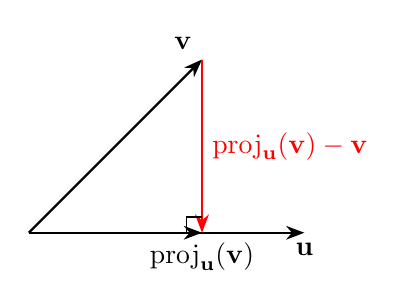
\begin{tikzpicture}[
    arr/.style={-{Stealth}, thick},
    redarr/.style={-{Stealth}, thick, red}
  ]
  \draw[arr] (0,0) -- (3.5,0) node[below] {$\mathbf{u}$};
  \draw[arr] (0,0) -- (2.2,2.2) node[above left] {$\mathbf{v}$};
  \draw[arr] (0,0) -- (2.2,0) node[below] {$\mathrm{proj}_{\mathbf{u}}(\mathbf{v})$};
  \draw[redarr] (2.2,2.2) -- (2.2,0) node[midway, right] {$\mathrm{proj}_{\mathbf{u}}(\mathbf{v})-\mathbf{v}$};
  \draw (2.0,0) -- (2.0,0.2) -- (2.2,0.2);
\end{tikzpicture}
\caption{The orthogonal projection of $\mathbf{v}$ onto $\mathbf{u}$. The residual
$\mathbf{v} - \mathrm{proj}_{\mathbf{u}}(\mathbf{v})$ is perpendicular to $\mathbf{u}$.}
\label{fig:orth-proj}
\end{figure}

\begin{proposition}[The residual is orthogonal to the base vector]
\label{prop:proj-residual-orth}
Let $(V,\langle\,\cdot,\cdot\,\rangle)$ be an inner product space and let
$\mathbf{u},\mathbf{v}\in V$ with $\mathbf{u}\neq\mathbf{0}_V$.
Then $\mathbf{u}\perp\bigl(\mathbf{v}-\mathrm{proj}_{\mathbf{u}}(\mathbf{v})\bigr)$.
\end{proposition}

\begin{proof}
\begin{align*}
  \Bigl\langle\mathbf{u},\,\mathbf{v}-\mathrm{proj}_{\mathbf{u}}(\mathbf{v})\Bigr\rangle
  &= \Bigl\langle\mathbf{u},\,\mathbf{v}-\frac{\langle\mathbf{u},\mathbf{v}\rangle}{\langle\mathbf{u},\mathbf{u}\rangle}\cdot\mathbf{u}\Bigr\rangle \\
  &= \langle\mathbf{u},\mathbf{v}\rangle
     - \frac{\langle\mathbf{u},\mathbf{v}\rangle}{\langle\mathbf{u},\mathbf{u}\rangle}\langle\mathbf{u},\mathbf{u}\rangle \\
  &= \langle\mathbf{u},\mathbf{v}\rangle - \langle\mathbf{u},\mathbf{v}\rangle = 0. \qedhere
\end{align*}
\end{proof}

\begin{remark}
Proposition~\ref{prop:proj-residual-orth} is illustrated in Figure~\ref{fig:orth-proj}:
$\mathrm{proj}_{\mathbf{u}}(\mathbf{v})$ is the component of $\mathbf{v}$ parallel to $\mathbf{u}$,
and $\mathbf{v}-\mathrm{proj}_{\mathbf{u}}(\mathbf{v})$ is the component of $\mathbf{v}$
perpendicular to $\mathbf{u}$.
\end{remark}

%================================================================
\section{The Gram--Schmidt Orthogonalization Process}
\label{sec:gram-schmidt}

\begin{theorem}[The Gram--Schmidt Orthogonalization Process]
\label{thm:gram-schmidt}
Let $(V,\langle\,\cdot,\cdot\,\rangle)$ be a finite-dimensional inner product space with
$\dim(V) = n\geq 1$, and let $\beta = (\mathbf{b}_1,\ldots,\mathbf{b}_n)$ be an ordered basis
for $V$.
Define a sequence $(\mathbf{v}_1,\ldots,\mathbf{v}_n)$ of $V$-vectors recursively by
\begin{align*}
  \mathbf{v}_1 &\;\stackrel{\mathrm{df}}{=}\; \mathbf{b}_1,\\
  \mathbf{v}_2 &\;\stackrel{\mathrm{df}}{=}\; \mathbf{b}_2 - \mathrm{proj}_{\mathbf{v}_1}(\mathbf{b}_2),\\
               &\;\;\vdots\\
  \mathbf{v}_k &\;\stackrel{\mathrm{df}}{=}\; \mathbf{b}_k
               - \mathrm{proj}_{\mathbf{v}_1}(\mathbf{b}_k)
               - \cdots
               - \mathrm{proj}_{\mathbf{v}_{k-1}}(\mathbf{b}_k),
               \quad k = 2,\ldots,n.
\end{align*}
Equivalently, expanding the projection formula
(Definition~\ref{def:orth-proj}):
\[
  \mathbf{v}_k = \mathbf{b}_k
    - \sum_{j=1}^{k-1}\frac{\langle\mathbf{v}_j,\mathbf{b}_k\rangle}{\langle\mathbf{v}_j,\mathbf{v}_j\rangle}\cdot\mathbf{v}_j,
  \qquad k = 2,\ldots,n.
\]
Then
\[
  \left\{\frac{1}{\|\mathbf{v}_1\|}\cdot\mathbf{v}_1,\;\ldots,\;\frac{1}{\|\mathbf{v}_n\|}\cdot\mathbf{v}_n\right\}
\]
is an orthonormal basis for $(V,\langle\,\cdot,\cdot\,\rangle)$.
\end{theorem}

\begin{proof}
For each $k\in\{1,\ldots,n\}$, let $P(k)$ denote the joint statement:
\[
  \begin{cases}
    \{\mathbf{v}_1,\ldots,\mathbf{v}_k\} \text{ is an orthogonal set of $k$ distinct non-zero vectors},\\
    \mathrm{Span}(\{\mathbf{v}_1,\ldots,\mathbf{v}_k\}) = \mathrm{Span}(\{\mathbf{b}_1,\ldots,\mathbf{b}_k\}).
  \end{cases}
\]
We prove $P(k)$ for all $k\in\{1,\ldots,n\}$ by induction.

\medskip
\textit{Base case} ($k=1$): $\mathbf{v}_1 = \mathbf{b}_1 \neq \mathbf{0}_V$ (since $\beta$ is a
basis) and $\mathrm{Span}(\{\mathbf{v}_1\}) = \mathrm{Span}(\{\mathbf{b}_1\})$, so $P(1)$ holds.

\medskip
\textit{Inductive step}: Suppose $k\in\{1,\ldots,n-1\}$ and $P(k)$ holds. We verify $P(k+1)$.

\textit{Step 1 ($\mathbf{v}_{k+1}\neq\mathbf{0}_V$).}
If $\mathbf{v}_{k+1} = \mathbf{0}_V$, then
\[
  \mathbf{b}_{k+1}
  = \sum_{j=1}^{k}\frac{\langle\mathbf{v}_j,\mathbf{b}_{k+1}\rangle}{\langle\mathbf{v}_j,\mathbf{v}_j\rangle}\cdot\mathbf{v}_j
  \;\in\; \mathrm{Span}(\{\mathbf{v}_1,\ldots,\mathbf{v}_k\})
  = \mathrm{Span}(\{\mathbf{b}_1,\ldots,\mathbf{b}_k\}),
\]
contradicting the linear independence of $\{\mathbf{b}_1,\ldots,\mathbf{b}_{k+1}\}$.
Hence $\mathbf{v}_{k+1}\neq\mathbf{0}_V$.

\textit{Step 2 (Span condition).}
Since $\mathbf{v}_{k+1} = \mathbf{b}_{k+1} - \sum_{j=1}^k c_j\mathbf{v}_j$ for some scalars $c_j$,
we have $\mathbf{v}_{k+1}\in\mathrm{Span}(\{\mathbf{b}_1,\ldots,\mathbf{b}_{k+1}\})$.
Similarly, $\mathbf{b}_{k+1} = \mathbf{v}_{k+1} + \sum_{j=1}^k c_j\mathbf{v}_j\in\mathrm{Span}(\{\mathbf{v}_1,\ldots,\mathbf{v}_{k+1}\})$.
Together with $P(k)$, this gives
$\mathrm{Span}(\{\mathbf{v}_1,\ldots,\mathbf{v}_{k+1}\}) = \mathrm{Span}(\{\mathbf{b}_1,\ldots,\mathbf{b}_{k+1}\})$.

\textit{Step 3 (Orthogonality).}
For each $i\in\{1,\ldots,k\}$, using linearity in the second argument and $P(k)$:
\begin{align*}
  \langle\mathbf{v}_i,\mathbf{v}_{k+1}\rangle
  &= \Bigl\langle\mathbf{v}_i,\,\mathbf{b}_{k+1}
     - \sum_{j=1}^k\frac{\langle\mathbf{v}_j,\mathbf{b}_{k+1}\rangle}{\langle\mathbf{v}_j,\mathbf{v}_j\rangle}\cdot\mathbf{v}_j\Bigr\rangle \\
  &= \langle\mathbf{v}_i,\mathbf{b}_{k+1}\rangle
     - \sum_{j=1}^k\frac{\langle\mathbf{v}_j,\mathbf{b}_{k+1}\rangle}{\langle\mathbf{v}_j,\mathbf{v}_j\rangle}\langle\mathbf{v}_i,\mathbf{v}_j\rangle \\
  &= \langle\mathbf{v}_i,\mathbf{b}_{k+1}\rangle
     - \frac{\langle\mathbf{v}_i,\mathbf{b}_{k+1}\rangle}{\langle\mathbf{v}_i,\mathbf{v}_i\rangle}\langle\mathbf{v}_i,\mathbf{v}_i\rangle = 0,
\end{align*}
where we used $\langle\mathbf{v}_i,\mathbf{v}_j\rangle = 0$ for $j\neq i$ (from $P(k)$).
Hence $P(k+1)$ holds.

\medskip
By induction, $P(k)$ holds for all $k$. In particular $P(n)$ says
$\{\mathbf{v}_1,\ldots,\mathbf{v}_n\}$ is an orthogonal set of $n$ non-zero vectors spanning $V$.
By Theorem~\ref{thm:orth-lin-indep} this set is linearly independent, hence a basis.
Dividing each $\mathbf{v}_k$ by its norm $\|\mathbf{v}_k\|$ yields a unit vector, producing
an orthonormal basis.
\end{proof}

\begin{keyresult}[title={Key Result: Gram--Schmidt Algorithm}]
Starting from any ordered basis $(\mathbf{b}_1,\ldots,\mathbf{b}_n)$, recursively set
$\mathbf{v}_k = \mathbf{b}_k - \sum_{j<k}\mathrm{proj}_{\mathbf{v}_j}(\mathbf{b}_k)$,
then normalize: $\mathbf{e}_k = \mathbf{v}_k/\|\mathbf{v}_k\|$.
The result $\{\mathbf{e}_1,\ldots,\mathbf{e}_n\}$ is an orthonormal basis.
\end{keyresult}

\begin{example}[Gram--Schmidt on $\mathscr{P}_2(\mathbb{R})$]
\label{ex:GS-P2}
Let $\langle P,Q\rangle \stackrel{\mathrm{df}}{=} \int_0^1 P\,Q$ be an inner product on
$\mathscr{P}_2(\mathbb{R})$.
Apply Gram--Schmidt to the standard ordered basis
$\sigma = (1,\,X,\,X^2)$ to obtain an orthonormal basis.

\medskip
\textbf{Step 1.} Set $\mathbf{v}_1 = 1$.
Then $\|\mathbf{v}_1\|^2 = \int_0^1 1\,\mathrm{d}x = 1$, so $\|\mathbf{v}_1\| = 1$
and $\mathbf{e}_1 = 1$.

\medskip
\textbf{Step 2.} Compute $\mathbf{v}_2 = X - \mathrm{proj}_{\mathbf{v}_1}(X)$:
\[
  \langle\mathbf{v}_1,X\rangle = \int_0^1 X\,\mathrm{d}x = \tfrac{1}{2},
  \qquad
  \langle\mathbf{v}_1,\mathbf{v}_1\rangle = 1,
\]
so $\mathrm{proj}_{\mathbf{v}_1}(X) = \tfrac{1}{2}\cdot 1 = \tfrac{1}{2}$
and $\mathbf{v}_2 = X - \tfrac{1}{2}$.
\[
  \|\mathbf{v}_2\|^2 = \int_0^1\!\Bigl(X-\tfrac{1}{2}\Bigr)^2\mathrm{d}x
  = \int_0^1\!\Bigl(X^2-X+\tfrac{1}{4}\Bigr)\mathrm{d}x
  = \tfrac{1}{3}-\tfrac{1}{2}+\tfrac{1}{4} = \tfrac{1}{12},
  \quad\text{so }\|\mathbf{v}_2\| = \tfrac{1}{2\sqrt{3}}.
\]
Hence $\mathbf{e}_2 = 2\sqrt{3}\,(X-\tfrac{1}{2}) = \sqrt{3}(2X-1)$.

\medskip
\textbf{Step 3.} Compute $\mathbf{v}_3 = X^2
   - \mathrm{proj}_{\mathbf{v}_1}(X^2) - \mathrm{proj}_{\mathbf{v}_2}(X^2)$:
\begin{align*}
  \langle\mathbf{v}_1,X^2\rangle &= \int_0^1 X^2\,\mathrm{d}x = \tfrac{1}{3},
  \quad\text{so }\mathrm{proj}_{\mathbf{v}_1}(X^2) = \tfrac{1}{3}.\\
  \langle\mathbf{v}_2,X^2\rangle &= \int_0^1\Bigl(X-\tfrac{1}{2}\Bigr)X^2\,\mathrm{d}x
    = \int_0^1\Bigl(X^3-\tfrac{X^2}{2}\Bigr)\mathrm{d}x
    = \tfrac{1}{4}-\tfrac{1}{6} = \tfrac{1}{12},\\
  \text{so }\mathrm{proj}_{\mathbf{v}_2}(X^2) &= \frac{1/12}{1/12}\cdot\Bigl(X-\tfrac{1}{2}\Bigr) = X-\tfrac{1}{2}.
\end{align*}
Therefore
\[
  \mathbf{v}_3 = X^2 - \tfrac{1}{3} - \Bigl(X-\tfrac{1}{2}\Bigr) = X^2 - X + \tfrac{1}{6}.
\]
\[
  \|\mathbf{v}_3\|^2 = \int_0^1\!\Bigl(X^2-X+\tfrac{1}{6}\Bigr)^2\mathrm{d}x
  = \int_0^1\!\Bigl(X^4-2X^3+\tfrac{4}{3}X^2-\tfrac{X}{3}+\tfrac{1}{36}\Bigr)\mathrm{d}x
  = \tfrac{1}{5}-\tfrac{1}{2}+\tfrac{4}{9}-\tfrac{1}{6}+\tfrac{1}{36}
  = \tfrac{1}{180}.
\]
Hence $\|\mathbf{v}_3\| = \tfrac{1}{6\sqrt{5}}$ and
$\mathbf{e}_3 = 6\sqrt{5}\,\bigl(X^2-X+\tfrac{1}{6}\bigr) = \sqrt{5}(6X^2-6X+1)$.

\medskip
\textbf{Conclusion.} An orthonormal basis for $(\mathscr{P}_2(\mathbb{R}),\langle\,\cdot,\cdot\,\rangle)$ is
\[
  \bigl\{1,\;\sqrt{3}(2X-1),\;\sqrt{5}(6X^2-6X+1)\bigr\}.
\]
\end{example}

\begin{examtip}[title={Exam Tip: Gram--Schmidt Workflow}]
Always compute and simplify $\langle\mathbf{v}_j,\mathbf{b}_{k+1}\rangle$ and
$\langle\mathbf{v}_j,\mathbf{v}_j\rangle$ separately before forming the projection.
Errors in $\|\mathbf{v}_j\|^2$ propagate into all later steps.
Check orthogonality of intermediate vectors before normalizing.
\end{examtip}

%================================================================
\chapter{Orthogonal Complements and Applications}
\label{chap:week12}

The previous chapter built up the geometry of an inner product space:
orthogonal sets, orthonormal bases, Fourier coefficients, projection
onto a single vector, and the Gram--Schmidt process for producing an
orthonormal basis. We now use these tools to study the
\emph{orthogonal complement} of a subset~$A$ of $V$ --- the set of all
vectors perpendicular to everything in~$A$. When $A$ is a finite-dimensional
subspace~$W$, the complement $W^\perp$ pairs with $W$ to decompose $V$
as the direct sum $W\oplus W^\perp$, and the resulting projection $P_W$
solves the geometric problem of finding the closest point in $W$ to a
given vector. We close the chapter --- and the course --- with two
applications: the Schr\"odinger equation as an eigenvalue problem on an
infinite-dimensional inner product space, and the method of linear
least-squares as an exercise in orthogonal projection onto a column space.

%================================================================
\section{Orthogonal Complements}
\label{sec:orth-complement}

%----------------------------------------------------------------
\subsection{Definition and First Examples}
\label{subsec:orth-comp-def}

\begin{definition}[Orthogonal complement]
\label{def:orth-complement}
Let $(V,\langle\,\cdot,\cdot\,\rangle)$ be an inner product space (not
necessarily finite-dimensional), and let $A$ be a \emph{non-empty} subset
of~$V$. The \emph{orthogonal complement} of $A$ with respect to
$(V,\langle\,\cdot,\cdot\,\rangle)$, denoted $A^\perp$, is the set
\[
  A^\perp \;\stackrel{\mathrm{df}}{=}\; \bigl\{\mathbf{v}\in V \;\bigm|\;
    \forall\,\mathbf{u}\in A\,:\, \mathbf{u}\perp\mathbf{v}\bigr\}
  \;=\; \bigl\{\mathbf{v}\in V \;\bigm|\;
    \forall\,\mathbf{u}\in A\,:\, \langle\mathbf{u},\mathbf{v}\rangle = 0\bigr\}.
\]
That is, $A^\perp$ is the set of all $V$-vectors orthogonal (in the sense of
Definition~\ref{def:orthogonal}) to every vector in~$A$.
\end{definition}

\begin{remark}
$A$ is \emph{not} required to be a vector subspace of~$V$. The complement
$A^\perp$ makes sense for any non-empty subset --- a single polynomial, a
finite list of vectors, an arbitrary set --- and as we are about to see,
$A^\perp$ is always a vector subspace of $V$ regardless of how $A$ looks.
\end{remark}

%----------------------------------------------------------------
\subsection{Orthogonal Complements are Vector Subspaces}
\label{subsec:orth-comp-subspace}

\begin{theorem}[Orthogonal complements are vector subspaces]
\label{thm:orth-comp-subspace}
Let $(V,\langle\,\cdot,\cdot\,\rangle)$ be an inner product space and let
$A$ be a non-empty subset of~$V$. Then $A^\perp$ is a vector subspace of~$V$.
\end{theorem}

\begin{proof}
We apply the Subspace Test (Key Result on page~\pageref{def:subspace}).
\begin{enumerate}
  \item \textit{Non-emptiness:} For every $\mathbf{u}\in A$ we have
        $\langle\mathbf{u},\mathbf{0}_V\rangle = 0$ (a property of inner
        products), so $\mathbf{0}_V\in A^\perp$ and $A^\perp\neq\varnothing$.
  \item \textit{Closure:} Let $\mathbf{v},\mathbf{w}\in A^\perp$ and let
        $\lambda$ be a scalar. For every $\mathbf{u}\in A$,
        \begin{align*}
          \langle\mathbf{u},\,\mathbf{v}+\mathbf{w}\rangle
            &= \langle\mathbf{u},\mathbf{v}\rangle + \langle\mathbf{u},\mathbf{w}\rangle
             = 0 + 0 = 0,\\
          \langle\mathbf{u},\,\lambda\cdot\mathbf{v}\rangle
            &= \lambda\,\langle\mathbf{u},\mathbf{v}\rangle = \lambda\cdot 0 = 0,
        \end{align*}
        so $\mathbf{v}+\mathbf{w}\in A^\perp$ and $\lambda\cdot\mathbf{v}\in A^\perp$.
\end{enumerate}
Hence $A^\perp$ is closed under addition and scalar multiplication, and is
therefore a vector subspace of~$V$.
\end{proof}

\begin{keyresult}[title={Key Result: $A^\perp$ is Always a Subspace}]
For \emph{any} non-empty subset $A$ of an inner product space $V$, the orthogonal
complement $A^\perp$ is a vector subspace of $V$ --- even when $A$ itself is just
a single vector or an unstructured set. In particular, $\mathbf{0}_V\in A^\perp$ always.
\end{keyresult}

%----------------------------------------------------------------
\subsection{Properties of Orthogonal Complements}
\label{subsec:orth-comp-properties}

\begin{theorem}[Properties of orthogonal complements]
\label{thm:orth-comp-properties}
Let $(V,\langle\,\cdot,\cdot\,\rangle)$ be an inner product space.
The following hold:
\begin{enumerate}
  \item $\{\mathbf{0}_V\}^\perp = V$.
  \item $V^\perp = \{\mathbf{0}_V\}$.
  \item For every non-empty subset $A$ of~$V$,
        $A\cap A^\perp \subseteq \{\mathbf{0}_V\}$.
  \item For all non-empty subsets $A, B$ of~$V$,
        $A\subseteq B \;\Longrightarrow\; B^\perp\subseteq A^\perp$.
  \item For every non-empty subset $A$ of~$V$,
        $A^\perp = \mathrm{Span}(A)^\perp$.
\end{enumerate}
\end{theorem}

\begin{proof}~

\textit{(1)} By definition,
$\{\mathbf{0}_V\}^\perp = \{\mathbf{v}\in V \mid \langle\mathbf{0}_V,\mathbf{v}\rangle = 0\} = V$,
since $\langle\mathbf{0}_V,\mathbf{v}\rangle = 0$ for all $\mathbf{v}\in V$.

\textit{(2)} By definition,
$V^\perp = \{\mathbf{v}\in V \mid \forall\,\mathbf{u}\in V\,:\, \langle\mathbf{u},\mathbf{v}\rangle = 0\}$.
Let $\mathbf{v}\in V^\perp$ be arbitrary. Then for all $\mathbf{u}\in V$ we have
$\langle\mathbf{u},\mathbf{v}\rangle = 0$. Taking $\mathbf{u} = \mathbf{v}$ gives
$\langle\mathbf{v},\mathbf{v}\rangle = 0$, which by positive-definiteness forces
$\mathbf{v} = \mathbf{0}_V$. Hence $V^\perp \subseteq \{\mathbf{0}_V\}$. The reverse
inclusion is immediate from~(1) (or directly: $\langle\mathbf{u},\mathbf{0}_V\rangle = 0$
for all $\mathbf{u}$). Therefore $V^\perp = \{\mathbf{0}_V\}$.

\textit{(3)} If $A\cap A^\perp = \varnothing$, then $A\cap A^\perp\subseteq\{\mathbf{0}_V\}$
trivially. Otherwise let $\mathbf{v}\in A\cap A^\perp$. Since $\mathbf{v}\in A^\perp$,
we have $\langle\mathbf{u},\mathbf{v}\rangle = 0$ for all $\mathbf{u}\in A$. Taking
$\mathbf{u} = \mathbf{v}\in A$ yields $\langle\mathbf{v},\mathbf{v}\rangle = 0$, so
$\mathbf{v} = \mathbf{0}_V$ by positive-definiteness. Hence $A\cap A^\perp \subseteq \{\mathbf{0}_V\}$.

\textit{(4)} Suppose $A\subseteq B$ and let $\mathbf{v}\in B^\perp$. Then
$\langle\mathbf{u},\mathbf{v}\rangle = 0$ for all $\mathbf{u}\in B$; in particular this holds for
all $\mathbf{u}\in A$, so $\mathbf{v}\in A^\perp$. Hence $B^\perp\subseteq A^\perp$.

\textit{(5)} Since $A\subseteq\mathrm{Span}(A)$, statement~(4) gives
$\mathrm{Span}(A)^\perp\subseteq A^\perp$. Conversely, let $\mathbf{v}\in A^\perp$;
we must show $\langle\mathbf{w},\mathbf{v}\rangle = 0$ for every $\mathbf{w}\in\mathrm{Span}(A)$.
Write $\mathbf{w} = \lambda_1\mathbf{u}_1 + \cdots + \lambda_n\mathbf{u}_n$ for some
$\mathbf{u}_1,\ldots,\mathbf{u}_n\in A$ and scalars $\lambda_1,\ldots,\lambda_n$. Then,
using conjugate-linearity in the first argument,
\[
  \langle\mathbf{w},\mathbf{v}\rangle
  = \Bigl\langle\sum_{k=1}^n\lambda_k\mathbf{u}_k,\,\mathbf{v}\Bigr\rangle
  = \sum_{k=1}^n\overline{\lambda_k}\langle\mathbf{u}_k,\mathbf{v}\rangle
  = \sum_{k=1}^n\overline{\lambda_k}\cdot 0 = 0,
\]
so $\mathbf{v}\in\mathrm{Span}(A)^\perp$. Hence $A^\perp\subseteq\mathrm{Span}(A)^\perp$,
and therefore $A^\perp = \mathrm{Span}(A)^\perp$.
\end{proof}

\begin{remark}
Property~(3) is the orthogonal analogue of the direct-sum criterion
(Definition~\ref{def:direct-sum}): a vector that is both \emph{in} a set
and \emph{perpendicular to it} can only be the zero vector. Property~(5)
is the workhorse: it converts any complement-of-a-set problem into a
complement-of-a-subspace problem.
\end{remark}

%----------------------------------------------------------------
\subsection{Computing Orthogonal Complements}
\label{subsec:orth-comp-procedure}

The following theorem, combined with property~(5) above, reduces
the computation of $A^\perp$ to a finite system of linear equations
whenever $\mathrm{Span}(A)$ is finite-dimensional.

\begin{theorem}[Computing the orthogonal complement of a subspace]
\label{thm:orth-comp-from-basis}
Let $(V,\langle\,\cdot,\cdot\,\rangle)$ be an inner product space (not
necessarily finite-dimensional), let $W$ be a vector subspace of~$V$, and
let $B$ be a basis for~$W$. Then
\[
  W^\perp \;=\; \bigl\{\mathbf{v}\in V \;\bigm|\;
    \forall\,\mathbf{b}\in B\,:\, \langle\mathbf{b},\mathbf{v}\rangle = 0\bigr\}.
\]
\end{theorem}

\begin{proof}
$(\subseteq)$ If $\mathbf{v}\in W^\perp$ then
$\langle\mathbf{u},\mathbf{v}\rangle = 0$ for all $\mathbf{u}\in W$;
since $B\subseteq W$, this in particular gives $\langle\mathbf{b},\mathbf{v}\rangle = 0$ for all $\mathbf{b}\in B$.

$(\supseteq)$ Conversely, suppose $\mathbf{v}\in V$ satisfies
$\langle\mathbf{b},\mathbf{v}\rangle = 0$ for every $\mathbf{b}\in B$. For an
arbitrary $\mathbf{w}\in W$, write $\mathbf{w} = \sum_{\mathbf{b}\in B}\lambda_\mathbf{b}\cdot\mathbf{b}$
(a finite sum, since basis representations are finite). Then
\[
  \langle\mathbf{w},\mathbf{v}\rangle
  = \Bigl\langle\sum_{\mathbf{b}\in B}\lambda_\mathbf{b}\cdot\mathbf{b},\,\mathbf{v}\Bigr\rangle
  = \sum_{\mathbf{b}\in B}\overline{\lambda_\mathbf{b}}\,\langle\mathbf{b},\mathbf{v}\rangle
  = \sum_{\mathbf{b}\in B}\overline{\lambda_\mathbf{b}}\cdot 0 = 0,
\]
so $\mathbf{v}\in W^\perp$.
\end{proof}

\begin{examtip}[title={Procedure: Finding $A^\perp$ for a Non-Empty Set $A$}]
Let $A$ be a non-empty subset of $V$.
\begin{enumerate}
  \item Replace $A$ by $\mathrm{Span}(A)$ using property~(5):
        $A^\perp = \mathrm{Span}(A)^\perp$.
  \item Pick a basis $B$ for $\mathrm{Span}(A)$. In practice, take $B$ to be any
        \emph{maximal linearly independent} subset of~$A$ --- if $V$ is
        finite-dimensional, ``maximal'' just means ``largest''.
  \item Solve the system of equations
        $\;\forall\,\mathbf{b}\in B\,:\,\langle\mathbf{b},\mathbf{v}\rangle = 0\;$
        for $\mathbf{v}\in V$. The solution set is $A^\perp$.
\end{enumerate}
If $B$ is finite, the system in step~3 is also finite --- one equation per basis vector.
\end{examtip}

%----------------------------------------------------------------
\subsection{Worked Example: A Singleton Subset of $\mathscr{P}_2(\mathbb{R})$}
\label{subsec:orth-comp-poly}

\begin{example}[Orthogonal complement of $\{1+X+X^2\}$]
\label{ex:orth-comp-poly}
Consider the real inner product space $(\mathscr{P}_2(\mathbb{R}),\langle\,\cdot,\cdot\,\rangle)$ where
\[
  \forall\, P,Q\in\mathscr{P}_2(\mathbb{R})\,:\quad
  \langle P,Q\rangle \stackrel{\mathrm{df}}{=} \int_{-1}^{1} P(x)Q(x)\,\mathrm{d}x.
\]
We derive a basis for $\{1+X+X^2\}^\perp$.

\smallskip
\noindent\emph{Step~1 (set up the equation).} A general element of
$\mathscr{P}_2(\mathbb{R})$ has the form $a + bX + cX^2$. We compute
$\langle 1+X+X^2,\,a+bX+cX^2\rangle$ and set it to zero:
\begin{align*}
  \int_{-1}^{1}(1+x+x^2)(a+bx+cx^2)\,\mathrm{d}x
  &= \int_{-1}^{1}\!\Bigl[a + (a+b)x + (a+b+c)x^2 + (b+c)x^3 + cx^4\Bigr]\mathrm{d}x.
\end{align*}
The odd-power terms integrate to zero on $[-1,1]$, leaving
\[
  2a + \tfrac{2}{3}(a+b+c) + \tfrac{2}{5}c \;=\; 0.
\]
Multiplying by~15 and simplifying,
\[
  30a + 10(a+b+c) + 6c = 0
  \;\Longleftrightarrow\; 40a + 10b + 16c = 0
  \;\Longleftrightarrow\; a = -\tfrac{1}{4}b - \tfrac{2}{5}c.
\]

\smallskip
\noindent\emph{Step~2 (parametrise the solution set).} Substituting back,
\begin{align*}
  \{1+X+X^2\}^\perp
    &= \bigl\{a + bX + cX^2 \,\bigm|\, a,b,c\in\mathbb{R},\;a = -\tfrac{1}{4}b - \tfrac{2}{5}c\bigr\}\\
    &= \bigl\{\bigl(-\tfrac{1}{4}b - \tfrac{2}{5}c\bigr) + bX + cX^2 \,\bigm|\, b,c\in\mathbb{R}\bigr\}\\
    &= \bigl\{b\bigl(-\tfrac{1}{4} + X\bigr) + c\bigl(-\tfrac{2}{5} + X^2\bigr) \,\bigm|\, b,c\in\mathbb{R}\bigr\}\\
    &= \mathrm{Span}\bigl(\bigl\{-\tfrac{1}{4}+X,\, -\tfrac{2}{5}+X^2\bigr\}\bigr)\\
    &= \mathrm{Span}\bigl(\bigl\{-1+4X,\, -2+5X^2\bigr\}\bigr)
    \quad\text{(rescaling each generator)}.
\end{align*}

\smallskip
\noindent\emph{Step~3 (verify linear independence).} Neither $-1+4X$ nor
$-2+5X^2$ is a scalar multiple of the other, so $\{-1+4X,\,-2+5X^2\}$ is
linearly independent and hence a basis for $\{1+X+X^2\}^\perp$.

\smallskip
\noindent\emph{Sanity check.} $\dim(\mathrm{Span}(\{1+X+X^2\})) = 1$ and
$\dim(\{1+X+X^2\}^\perp) = 2$, summing to $3 = \dim(\mathscr{P}_2(\mathbb{R}))$
--- consistent with the direct-sum decomposition we are about to prove.
\end{example}

%================================================================
\section{Direct-Sum Decomposition and Orthogonal Projection}
\label{sec:direct-sum-decomp}

%----------------------------------------------------------------
\subsection{The Decomposition $V = W\oplus W^\perp$}
\label{subsec:direct-sum-decomp}

\begin{theorem}[A subspace and its orthogonal complement form a direct sum]
\label{thm:direct-sum-decomp}
Let $(V,\langle\,\cdot,\cdot\,\rangle)$ be a \emph{finite-dimensional}
inner product space and let $W$ be a vector subspace of~$V$. Then
\[
  V \;=\; W\,\oplus\, W^\perp,
\]
and consequently $\dim(V) = \dim(W) + \dim(W^\perp)$.
\end{theorem}

\begin{proof}
By the Gram--Schmidt Orthogonalization Process
(Theorem~\ref{thm:gram-schmidt}), the subspace $W$ admits an orthonormal
basis $B = \{\mathbf{b}_1,\ldots,\mathbf{b}_m\}$ where $m = \dim(W)$.
Let $\mathbf{v}\in V$ be arbitrary, and define
\[
  \mathbf{p} \;\stackrel{\mathrm{df}}{=}\; \sum_{k=1}^{m}\langle\mathbf{b}_k,\mathbf{v}\rangle\cdot\mathbf{b}_k
  \quad\text{and}\quad
  \mathbf{q} \;\stackrel{\mathrm{df}}{=}\; \mathbf{v} - \mathbf{p}.
\]
The coefficients $\langle\mathbf{b}_k,\mathbf{v}\rangle$ are the
$B$-Fourier coefficients of $\mathbf{v}$ (Definition~\ref{def:fourier-coeffs}).
Plainly $\mathbf{p}\in\mathrm{Span}(B) = W$, and $\mathbf{v} = \mathbf{p}+\mathbf{q}$
by construction.

\smallskip
\noindent\textit{Claim: $\mathbf{q}\in W^\perp$.} For any $\mathbf{w}\in W$
we may write $\mathbf{w} = \sum_{j=1}^{m}\lambda_j\mathbf{b}_j$, and then
\begin{align*}
  \langle\mathbf{w},\mathbf{q}\rangle
    &= \langle\mathbf{w},\mathbf{v}\rangle - \langle\mathbf{w},\mathbf{p}\rangle\\
    &= \Bigl\langle\sum_{j=1}^{m}\lambda_j\mathbf{b}_j,\mathbf{v}\Bigr\rangle
       - \Bigl\langle\sum_{j=1}^{m}\lambda_j\mathbf{b}_j,\,\sum_{k=1}^{m}\langle\mathbf{b}_k,\mathbf{v}\rangle\mathbf{b}_k\Bigr\rangle\\
    &= \sum_{j=1}^{m}\overline{\lambda_j}\langle\mathbf{b}_j,\mathbf{v}\rangle
       - \sum_{j,k=1}^{m}\overline{\lambda_j}\langle\mathbf{b}_k,\mathbf{v}\rangle\langle\mathbf{b}_j,\mathbf{b}_k\rangle.
\end{align*}
Orthonormality of $B$ gives $\langle\mathbf{b}_j,\mathbf{b}_k\rangle = \delta_{jk}$,
so the double sum collapses to $\sum_{j=1}^{m}\overline{\lambda_j}\langle\mathbf{b}_j,\mathbf{v}\rangle$,
which cancels the first term. Hence $\langle\mathbf{w},\mathbf{q}\rangle = 0$
for all $\mathbf{w}\in W$, i.e.\ $\mathbf{q}\in W^\perp$.

\smallskip
We have shown $V = W + W^\perp$. By property~(3) of
Theorem~\ref{thm:orth-comp-properties}, $W\cap W^\perp\subseteq\{\mathbf{0}_V\}$,
and the reverse inclusion is immediate (the zero vector lies in every subspace).
Hence $W\cap W^\perp = \{\mathbf{0}_V\}$, and the sum is direct:
$V = W\oplus W^\perp$. The dimension formula follows from the dimension
formula for direct sums.
\end{proof}

\begin{warning}[title={Warning: Finite-Dimensionality is Essential}]
Theorem~\ref{thm:direct-sum-decomp} can fail when $V$ is infinite-dimensional.
The proof relied on Gram--Schmidt producing a finite orthonormal basis for~$W$;
without finite dimension, $W^\perp$ may be smaller than expected and
$W + W^\perp$ may fail to exhaust~$V$. (The remedy in the infinite-dimensional
setting requires \emph{closed} subspaces and Hilbert space machinery, beyond
the scope of MH1201.)
\end{warning}

\begin{figure}[h]
\centering
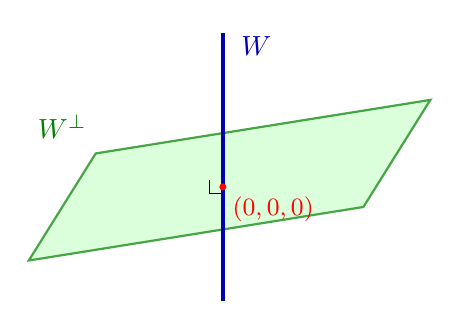
\begin{tikzpicture}[scale=0.85,
    plane/.style={fill=green!20, draw=green!50!black, thick, opacity=0.7},
    line/.style={draw=blue!70!black, very thick}
  ]
  % The plane W^perp
  \draw[plane] (-2.5,-1.4) -- (2.5,-0.6) -- (3.5,1) -- (-1.5,0.2) -- cycle;
  \node[green!50!black] at (-2.0,0.6) {$W^\perp$};
  % The line W (vertical)
  \draw[line] (0.4,-2.0) -- (0.4,2.0);
  \node[blue!70!black] at (0.9,1.8) {$W$};
  % Origin
  \fill[red] (0.4,-0.3) circle (1.5pt);
  \node[red, below right] at (0.4,-0.3) {\small$(0,0,0)$};
  % Right-angle marker at origin
  \draw[black, thin] (0.2,-0.2) -- (0.2,-0.4) -- (0.4,-0.4);
\end{tikzpicture}
\caption{Geometric picture of $\mathbb{R}^3 = W\oplus W^\perp$ with
$\dim(W) = 1$ and $\dim(W^\perp) = 2$. Every vector in~$\mathbb{R}^3$ decomposes
uniquely as a sum of a vector along the line~$W$ and a vector in the plane~$W^\perp$.}
\label{fig:direct-sum-R3}
\end{figure}

%----------------------------------------------------------------
\subsection{The Orthogonal Projection Operator}
\label{subsec:orth-proj-operator}

The unique decomposition $\mathbf{v} = \mathbf{p} + \mathbf{q}$ from
Theorem~\ref{thm:direct-sum-decomp} extracts a well-defined
$W$-component~$\mathbf{p}$ from each $\mathbf{v}\in V$. The map sending
$\mathbf{v}$ to that component is the orthogonal projection onto~$W$.

\begin{definition}[Orthogonal projection operator onto a subspace]
\label{def:orth-proj-operator}
Let $(V,\langle\,\cdot,\cdot\,\rangle)$ be a finite-dimensional inner
product space and let $W$ be a vector subspace of~$V$. The
\emph{orthogonal projection operator onto~$W$}, denoted $P_W$, is the
linear transformation $P_W : V \to W$ that maps each $\mathbf{v}\in V$ to its
$W$-component in the decomposition $V = W\oplus W^\perp$.
\end{definition}

\begin{remark}
Definition~\ref{def:orth-proj-operator} generalizes the projection of a
vector onto another vector (Definition~\ref{def:orth-proj}): if
$W = \mathrm{Span}(\{\mathbf{u}\})$ for some non-zero $\mathbf{u}$, then
$P_W(\mathbf{v}) = \mathrm{proj}_{\mathbf{u}}(\mathbf{v})$. The new
definition extends the same idea to subspaces of arbitrary (finite) dimension.
If $\{\mathbf{b}_1,\ldots,\mathbf{b}_m\}$ is an orthonormal basis for $W$,
the proof of Theorem~\ref{thm:direct-sum-decomp} gives the explicit formula
\[
  P_W(\mathbf{v}) = \sum_{k=1}^{m}\langle\mathbf{b}_k,\mathbf{v}\rangle\cdot\mathbf{b}_k.
\]
\end{remark}

\begin{theorem}[The shortest distance from a point to a subspace]
\label{thm:shortest-distance}
Let $(V,\langle\,\cdot,\cdot\,\rangle)$ be a finite-dimensional inner
product space, let $W$ be a vector subspace of~$V$, and let $\mathbf{v}\in V$.
\begin{enumerate}
  \item There is precisely one $\mathbf{w}\in W$ closest to $\mathbf{v}$ in the
        norm induced by the inner product, namely $\mathbf{w} = P_W(\mathbf{v})$.
        This is also the unique $\mathbf{w}\in W$ for which $\mathbf{v}-\mathbf{w}\in W^\perp$.
  \item Consequently, the shortest distance from $\mathbf{v}$ to $W$ is
        $\|\mathbf{v} - P_W(\mathbf{v})\|$. If $\mathbf{v}$ already lies in~$W$
        then $P_W(\mathbf{v}) = \mathbf{v}$ and the distance is $0$.
\end{enumerate}
\end{theorem}

The proof, which is not examinable in MH1201, follows from a Pythagoras-style
argument: for any $\mathbf{w}\in W$, write $\mathbf{v} - \mathbf{w} = (\mathbf{v} - P_W(\mathbf{v})) + (P_W(\mathbf{v}) - \mathbf{w})$,
note that the first summand lies in $W^\perp$ and the second in~$W$, and apply
the Pythagorean identity $\|\mathbf{a}+\mathbf{b}\|^2 = \|\mathbf{a}\|^2 + \|\mathbf{b}\|^2$
when $\mathbf{a}\perp\mathbf{b}$.

\begin{figure}[h]
\centering
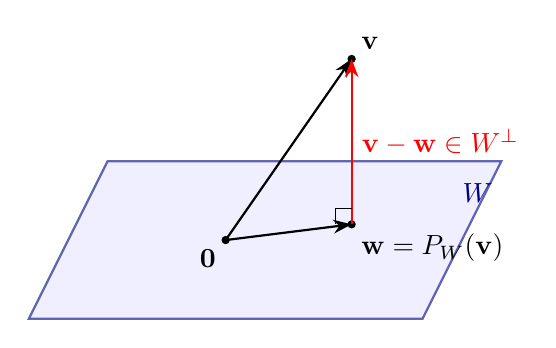
\begin{tikzpicture}[scale=1.0,
    plane/.style={fill=blue!10, draw=blue!50!black, thick, opacity=0.6},
    arr/.style={-{Stealth}, thick},
    redarr/.style={-{Stealth}, thick, red}
  ]
  % Plane W
  \draw[plane] (-2.5,-1) -- (2.5,-1) -- (3.5,1) -- (-1.5,1) -- cycle;
  \node[blue!50!black] at (3.2,0.6) {$W$};
  % Origin
  \coordinate (O) at (0,0);
  \fill[black] (O) circle (1.5pt);
  \node[below left] at (O) {$\mathbf{0}$};
  % w = P_W(v) in the plane
  \coordinate (w) at (1.6,0.2);
  \fill[black] (w) circle (1.5pt);
  \node[below right] at (w) {$\mathbf{w} = P_W(\mathbf{v})$};
  % v above the plane
  \coordinate (v) at (1.6,2.3);
  \fill[black] (v) circle (1.5pt);
  \node[above right] at (v) {$\mathbf{v}$};
  % arrows
  \draw[arr] (O) -- (v);
  \draw[arr] (O) -- (w);
  \draw[redarr] (w) -- (v) node[midway, right] {$\mathbf{v}-\mathbf{w}\in W^\perp$};
  % right angle marker
  \draw (1.4,0.2) -- (1.4,0.4) -- (1.6,0.4);
\end{tikzpicture}
\caption{The orthogonal projection $P_W(\mathbf{v})$ is the unique point in $W$
closest to $\mathbf{v}$. The residual $\mathbf{v} - P_W(\mathbf{v})$ is orthogonal
to every vector in $W$.}
\label{fig:orth-proj-operator}
\end{figure}

\begin{keyresult}[title={Key Result: Closest Point in a Subspace}]
For a finite-dimensional subspace $W$ of an inner product space $V$,
the unique point of $W$ closest to a given $\mathbf{v}\in V$ is the
orthogonal projection $P_W(\mathbf{v})$, characterised by the perpendicularity
condition $\mathbf{v} - P_W(\mathbf{v})\in W^\perp$. This is the geometric
fact that drives both Fourier-style approximation (Chapter~\ref{chap:week11})
and the linear least-squares method of Section~\ref{sec:applications}.
\end{keyresult}

%----------------------------------------------------------------
\subsection{Worked Example: A Matrix-Induced Inner Product on $\mathbb{R}^{4,1}$}
\label{subsec:orth-comp-R41}

\begin{example}[Decomposition with respect to a matrix-induced inner product]
\label{ex:orth-comp-R41}
Define $\langle\,\cdot,\cdot\,\rangle : \mathbb{R}^{4,1}\times\mathbb{R}^{4,1}\to\mathbb{R}$ by
\[
  \forall\,\mathbf{x},\mathbf{y}\in\mathbb{R}^{4,1}\,:\quad
  \langle\mathbf{x},\mathbf{y}\rangle \stackrel{\mathrm{df}}{=}
  \mathbf{x}^\top \mathbf{A}\,\mathbf{y},
  \qquad
  \mathbf{A} \stackrel{\mathrm{df}}{=}
  \begin{bmatrix} 4 & 0 & 2 & 0\\ 0 & 5 & 0 & 2\\ 2 & 0 & 6 & 0\\ 0 & 2 & 0 & 7 \end{bmatrix}.
\]
Let $W = \mathrm{Span}\bigl(\{\mathbf{e}_1,\mathbf{e}_3\}\bigr)$ where
$\mathbf{e}_1 = (1,0,0,0)^\top$ and $\mathbf{e}_3 = (0,0,1,0)^\top$.

\begin{enumerate}
  \item \textbf{$\langle\,\cdot,\cdot\,\rangle$ is an inner product on
        $\mathbb{R}^{4,1}$.} Note that $\mathbf{A}^\top = \mathbf{A}$.

        \emph{Linearity in the second argument.} For all $\mathbf{u},\mathbf{v},\mathbf{w}\in\mathbb{R}^{4,1}$ and $\lambda\in\mathbb{R}$,
        \[
          \langle\mathbf{u},\mathbf{v}+\lambda\mathbf{w}\rangle
          = \mathbf{u}^\top\mathbf{A}(\mathbf{v}+\lambda\mathbf{w})
          = \mathbf{u}^\top\mathbf{A}\mathbf{v} + \lambda\,\mathbf{u}^\top\mathbf{A}\mathbf{w}
          = \langle\mathbf{u},\mathbf{v}\rangle + \lambda\langle\mathbf{u},\mathbf{w}\rangle.
        \]

        \emph{Symmetry.} For all $\mathbf{u},\mathbf{v}\in\mathbb{R}^{4,1}$,
        \[
          \langle\mathbf{u},\mathbf{v}\rangle
          = \mathbf{u}^\top\mathbf{A}\mathbf{v}
          = (\mathbf{u}^\top\mathbf{A}\mathbf{v})^\top
          = \mathbf{v}^\top\mathbf{A}^\top\mathbf{u}
          = \mathbf{v}^\top\mathbf{A}\mathbf{u}
          = \langle\mathbf{v},\mathbf{u}\rangle,
        \]
        using that $\mathbf{u}^\top\mathbf{A}\mathbf{v}$ is a $1\times 1$ matrix and is therefore self-transpose.

        \emph{Positive-definiteness.} For $\mathbf{x} = (w,x,y,z)^\top$,
        \[
          \langle\mathbf{x},\mathbf{x}\rangle
          = 4w^2 + 5x^2 + 6y^2 + 7z^2 + 4wy + 4xz.
        \]
        Completing squares gives
        \[
          \langle\mathbf{x},\mathbf{x}\rangle
          = (2w + y)^2 + (2x + z)^2 + x^2 + 5y^2 + 6z^2 \;\geq\; 0,
        \]
        with equality iff $2w+y = 2x+z = x = y = z = 0$, i.e.\ iff
        $\mathbf{x} = \mathbf{0}$. Hence $\langle\,\cdot,\cdot\,\rangle$ is an inner product.

  \item \textbf{Basis for $W^\perp$.} By Theorem~\ref{thm:orth-comp-from-basis},
        $\mathbf{x} = (w,x,y,z)^\top\in W^\perp$ iff
        $\langle\mathbf{e}_1,\mathbf{x}\rangle = 0$ and $\langle\mathbf{e}_3,\mathbf{x}\rangle = 0$.
        Computing $\mathbf{e}_1^\top\mathbf{A} = (4,0,2,0)$ and $\mathbf{e}_3^\top\mathbf{A} = (2,0,6,0)$,
        the system becomes
        \[
          4w + 2y = 0,
          \qquad 2w + 6y = 0
          \;\;\Longleftrightarrow\;\; w = y = 0.
        \]
        Hence
        \[
          W^\perp = \bigl\{(0,x,0,z)^\top \,\bigm|\, x,z\in\mathbb{R}\bigr\}
                  = \mathrm{Span}\bigl(\{\mathbf{e}_2,\mathbf{e}_4\}\bigr),
        \]
        and $\{\mathbf{e}_2,\mathbf{e}_4\}$ --- linearly independent --- is a basis for $W^\perp$.

  \item \textbf{Decomposing $(1,2,3,4)^\top$.} Since $W$ is spanned by
        $\mathbf{e}_1,\mathbf{e}_3$ and $W^\perp$ by $\mathbf{e}_2,\mathbf{e}_4$, we read off
        \[
          \begin{bmatrix}1\\2\\3\\4\end{bmatrix}
          = \underbrace{\begin{bmatrix}1\\0\\3\\0\end{bmatrix}}_{\mathbf{p}\in W}
          + \underbrace{\begin{bmatrix}0\\2\\0\\4\end{bmatrix}}_{\mathbf{q}\in W^\perp}.
        \]
        That is, $\mathbf{p} = (1,0,3,0)^\top$ and $\mathbf{q} = (0,2,0,4)^\top$. Note
        that $\mathbf{p} = P_W\bigl((1,2,3,4)^\top\bigr)$.
\end{enumerate}
\end{example}

\begin{remark}
The decomposition in part~3 worked out cleanly because the $W$-basis
$\{\mathbf{e}_1,\mathbf{e}_3\}$ and the $W^\perp$-basis $\{\mathbf{e}_2,\mathbf{e}_4\}$
together form the standard basis of $\mathbb{R}^{4,1}$. In a different
inner product or with a different $W$, finding the $W$-component of a vector
typically requires the Fourier-coefficient formula
$P_W(\mathbf{v}) = \sum_k\langle\mathbf{b}_k,\mathbf{v}\rangle\mathbf{b}_k$
applied to an \emph{orthonormal} basis~$B$ of~$W$.
\end{remark}

%----------------------------------------------------------------
\subsection{Worked Example: Upper-Triangular Matrices}
\label{subsec:orth-comp-upper-triangular}

\begin{example}[Orthogonal complement of upper-triangular matrices]
\label{ex:orth-comp-upper-triangular}
Fix $n\in\mathbb{N}$ and consider the real inner product space
$(\mathbb{R}^{n,n},\langle\,\cdot,\cdot\,\rangle_F)$ where $\langle\,\cdot,\cdot\,\rangle_F$ is
the Frobenius inner product (Example~\ref{ex:frobenius-real}). Let
\[
  U \;\stackrel{\mathrm{df}}{=}\; \bigl\{\mathbf{A}\in\mathbb{R}^{n,n} \,\bigm|\, \mathbf{A}\text{ is upper-triangular}\bigr\}.
\]
We derive a basis for $U^\perp$.

\smallskip
$U$ is a vector subspace of $\mathbb{R}^{n,n}$ with basis
$\{\mathbf{E}^{a,b} \,|\, a,b\in\{1,\ldots,n\},\ a\leq b\}$, where
$\mathbf{E}^{a,b}$ is the standard basis matrix with a $1$ in position
$(a,b)$ and zeros elsewhere. (For $n=4$ this basis has 10 elements:
$\mathbf{E}^{1,1},\mathbf{E}^{1,2},\mathbf{E}^{1,3},\mathbf{E}^{1,4},\mathbf{E}^{2,2},\mathbf{E}^{2,3},\mathbf{E}^{2,4},\mathbf{E}^{3,3},\mathbf{E}^{3,4},\mathbf{E}^{4,4}$.)

By Theorem~\ref{thm:orth-comp-from-basis},
\[
  U^\perp = \bigl\{\mathbf{B}\in\mathbb{R}^{n,n} \,\bigm|\,
    \forall\,a,b\in\{1,\ldots,n\}\text{ s.t.\ }a\leq b\,:\, \langle\mathbf{E}^{a,b},\mathbf{B}\rangle_F = 0\bigr\}.
\]
We compute the inner product. By definition $\langle\mathbf{E}^{a,b},\mathbf{B}\rangle_F = \mathrm{trace}\bigl((\mathbf{E}^{a,b})^\top\mathbf{B}\bigr)$,
and expanding the trace and the matrix product,
\[
  \langle\mathbf{E}^{a,b},\mathbf{B}\rangle_F
  = \sum_{i=1}^{n}\sum_{j=1}^{n}\mathbf{E}^{a,b}[j,i]\,\mathbf{B}[j,i].
\]
But $\mathbf{E}^{a,b}[j,i] = 1$ iff $j=a$ and $i=b$ (and $0$ otherwise), so the
double sum collapses to the single entry $\mathbf{B}[a,b]$:
\[
  \langle\mathbf{E}^{a,b},\mathbf{B}\rangle_F = \mathbf{B}[a,b].
\]
Hence
\[
  U^\perp = \bigl\{\mathbf{B}\in\mathbb{R}^{n,n} \,\bigm|\,
    \forall\,a\leq b\,:\, \mathbf{B}[a,b] = 0\bigr\},
\]
which is precisely the subspace of \emph{strictly lower-triangular}
matrices. A basis for $U^\perp$ is therefore
\[
  \bigl\{\mathbf{E}^{c,d} \,\bigm|\, c,d\in\{1,\ldots,n\},\, c > d\bigr\}.
\]
For $n=4$ this gives the six matrices
$\{\mathbf{E}^{2,1},\mathbf{E}^{3,1},\mathbf{E}^{3,2},\mathbf{E}^{4,1},\mathbf{E}^{4,2},\mathbf{E}^{4,3}\}$,
matching the count $\dim(\mathbb{R}^{4,4}) - \dim(U) = 16 - 10 = 6$ predicted by
Theorem~\ref{thm:direct-sum-decomp}.
\end{example}

%================================================================
\section{Some Applications of Linear Algebra}
\label{sec:applications}

We close the course with two applications of the eigenvalue/orthogonality
machinery developed in Chapters~\ref{chap:week11}--\ref{chap:week12}.
The first is a famous problem from quantum mechanics; the second, a
data-fitting technique used everywhere from statistics to machine learning.

%----------------------------------------------------------------
\subsection{Quantum Mechanics: The Schr\"odinger Equation}
\label{subsec:schrodinger}

In the early development of quantum mechanics, one of the central challenges
was to predict the spectral frequencies of the hydrogen atom from a coherent
theoretical framework. Erwin Schr\"odinger resolved this with what is now
called the \emph{Time-Independent Schr\"odinger Equation}, an
\textbf{eigenvalue--eigenvector equation} on the (infinite-dimensional)
complex inner product space of wave-functions.

For the hydrogen atom, the equation reads
\[
  \underbrace{\left[
    -\frac{h^2}{8\pi^2\bigl(\tfrac{m_e m_p}{m_e + m_p}\bigr)}
    \left(\frac{\partial^2}{\partial x^2}+\frac{\partial^2}{\partial y^2}+\frac{\partial^2}{\partial z^2}\right)
    -\frac{1}{4\pi\varepsilon_0}\frac{e^2}{\sqrt{x^2+y^2+z^2}}
  \right]}_{\text{the Schr\"odinger operator for the hydrogen atom}}
  \psi \;=\; E\cdot\psi,
\]
where $m_e, m_p$ are the electron and proton masses, $e$ is the elementary
charge, $\varepsilon_0$ is the vacuum permittivity, $h$ is Planck's constant,
$E\in\mathbb{R}$ is the energy eigenvalue, and $\psi$ is a non-zero
eigenvector ---a wave-function--- in the complex vector space of
square-integrable wave-functions.

Solving this equation produces the discrete sequence of eigenvalues
\[
  \forall\,n\in\mathbb{N}\,:\quad
  E_n = -\frac{m_e e^4}{8\varepsilon_0^2 h^2 n^2}.
\]
These match the experimentally measured energy levels of the hydrogen
atom essentially exactly --- a striking confirmation that the algebraic
framework of eigenvalues, eigenvectors, and inner product spaces describes
physical reality.

\begin{remark}
The Schr\"odinger operator is a linear operator on an infinite-dimensional
complex inner product space, so the eigenvalue theory of
Chapter~\ref{chap:week8} applies in spirit but not
literally: the matrix-based proofs (e.g.\ via the characteristic polynomial)
do not work, and one must work directly with the operator equation.
Theorem~\ref{thm:direct-sum-decomp} also fails in general for such spaces ---
see the warning above. Nonetheless, the linear-algebraic vocabulary
(\emph{eigenvalue}, \emph{eigenvector}, \emph{inner product}, \emph{orthogonality})
remains exactly the right one.
\end{remark}

%----------------------------------------------------------------
\subsection{Statistics: Linear Least-Squares Approximation}
\label{subsec:lls}

Given $n$ distinct data points $(x_1,y_1),\ldots,(x_n,y_n)$ in $\mathbb{R}^2$,
we want to find the linear function $f:\mathbb{R}\to\mathbb{R}$,
$f(x) = mx + c$, that ``best fits'' the data in the sense of minimizing
the sum of squared vertical errors:
\[
  E_f \;\stackrel{\mathrm{df}}{=}\; \sum_{k=1}^{n}\bigl|y_k - f(x_k)\bigr|^2.
\]
Any $f$ that minimizes $E_f$ is called a \emph{linear least-squares
approximation} (LLS approximation) to the data points, and $E_f$ itself is
called the \emph{linear least-squares error} of~$f$.

% [Figure, Slide 24: a scatter plot of three data points (x_1,y_1),(x_2,y_2),(x_3,y_3)
%  with a fitted line f(x) and vertical residuals d_1, d_2, d_3 marked between each
%  point and the line. The figure motivates E_f as the sum of squared d_k.]
Geometrically, the picture is a scatter plot with a candidate fit-line
$f(x)$; the vertical distances $d_k = |y_k - f(x_k)|$ from each data point
to the line are the \emph{residuals}, and $E_f = \sum_k d_k^2$.

\smallskip
\noindent\textbf{Reformulation as a projection problem.} Set
\[
  \mathbf{y} \;\stackrel{\mathrm{df}}{=}\;
  \begin{bmatrix}y_1\\\vdots\\y_n\end{bmatrix}\in\mathbb{R}^{n,1},
  \qquad
  \mathbf{A} \;\stackrel{\mathrm{df}}{=}\;
  \begin{bmatrix}x_1 & 1\\ \vdots & \vdots \\ x_n & 1\end{bmatrix}\in\mathbb{R}^{n,2}.
\]
Then $\mathbf{A}\begin{bmatrix}m\\c\end{bmatrix} = (mx_1+c,\,\ldots,\,mx_n+c)^\top$
is the vector whose $k$th entry is $f(x_k)$, and so
\[
  E_f
  = \sum_{k=1}^{n}|y_k - mx_k - c|^2
  = \left\|\mathbf{y} - \mathbf{A}\begin{bmatrix}m\\c\end{bmatrix}\right\|^2.
\]
Define $W \stackrel{\mathrm{df}}{=} \{\mathbf{A}\mathbf{b} \,|\, \mathbf{b}\in\mathbb{R}^{2,1}\}$,
the column space of $\mathbf{A}$ --- a vector subspace of $\mathbb{R}^{n,1}$.
Minimizing $E_f$ over $(m,c)$ is precisely the problem of finding the point
in $W$ closest to $\mathbf{y}$, which by Theorem~\ref{thm:shortest-distance}
is the orthogonal projection $P_W(\mathbf{y})$.

\begin{theorem}[Three equivalent characterisations of an LLS solution]
\label{thm:lls-equivalence}
With $\mathbf{y}, \mathbf{A}, W$ as above, the following statements about
$\begin{bmatrix}m\\c\end{bmatrix}\in\mathbb{R}^{2,1}$ are equivalent:
\begin{enumerate}
  \item $\begin{bmatrix}m\\c\end{bmatrix}$ minimizes $E_f$.
  \item The point in $W$ that $\mathbf{y}$ is closest to is
        $\mathbf{A}\begin{bmatrix}m\\c\end{bmatrix}$;
        equivalently, $\mathbf{y} - \mathbf{A}\begin{bmatrix}m\\c\end{bmatrix}\in W^\perp$.
  \item $\mathbf{A}^\top\mathbf{A}\begin{bmatrix}m\\c\end{bmatrix} = \mathbf{A}^\top\mathbf{y}$
        (the \emph{normal equations}).
\end{enumerate}
\end{theorem}

\begin{proof}
$(1)\Leftrightarrow(2)$: Since $E_f = \|\mathbf{y} - \mathbf{A}[m,c]^\top\|^2$
and $\mathbf{A}[m,c]^\top$ ranges over all of $W$ as $(m,c)$ ranges over
$\mathbb{R}^{2,1}$, minimizing $E_f$ is the same as finding the point of $W$
closest to $\mathbf{y}$. By Theorem~\ref{thm:shortest-distance}, this point
is unique and characterised by the residual lying in $W^\perp$.

$(2)\Leftrightarrow(3)$: The condition $\mathbf{y} - \mathbf{A}[m,c]^\top\in W^\perp$
says, by Theorem~\ref{thm:orth-comp-from-basis} applied to the spanning set
of columns of $\mathbf{A}$,
\[
  \forall\,\mathbf{b}\in\mathbb{R}^{2,1}\,:\quad \langle\mathbf{A}\mathbf{b},\,\mathbf{y} - \mathbf{A}[m,c]^\top\rangle = 0.
\]
With the standard dot product on $\mathbb{R}^{n,1}$, this becomes
$(\mathbf{A}\mathbf{b})^\top(\mathbf{y} - \mathbf{A}[m,c]^\top) = 0$, i.e.\
$\mathbf{b}^\top\mathbf{A}^\top(\mathbf{y} - \mathbf{A}[m,c]^\top) = 0$, for every $\mathbf{b}\in\mathbb{R}^{2,1}$.
This forces $\mathbf{A}^\top(\mathbf{y} - \mathbf{A}[m,c]^\top) = \mathbf{0}$, which rearranges to
$\mathbf{A}^\top\mathbf{A}[m,c]^\top = \mathbf{A}^\top\mathbf{y}$.
\end{proof}

\begin{keyresult}[title={Key Result: The Normal Equations}]
The linear least-squares fit $f(x) = mx + c$ to data points
$(x_1,y_1),\ldots,(x_n,y_n)$ is found by solving
\[
  \mathbf{A}^\top\mathbf{A}\begin{bmatrix}m\\c\end{bmatrix} = \mathbf{A}^\top\mathbf{y},
  \qquad
  \mathbf{A} = \begin{bmatrix}x_1 & 1\\\vdots & \vdots\\ x_n & 1\end{bmatrix},\;
  \mathbf{y} = \begin{bmatrix}y_1\\\vdots\\y_n\end{bmatrix}.
\]
This is a $2\times 2$ linear system in $(m,c)$, solvable by any standard method;
the solution exists and is unique whenever the $x_k$ are not all equal (so that
the columns of $\mathbf{A}$ are linearly independent and $\mathbf{A}^\top\mathbf{A}$
is invertible).
\end{keyresult}

\begin{remark}
The same machinery extends without modification to higher-degree polynomial
fits, multivariate regression, and more general LLS problems: replace the
two-column matrix $\mathbf{A}$ with the appropriate design matrix, and the
normal equations $\mathbf{A}^\top\mathbf{A}\mathbf{x} = \mathbf{A}^\top\mathbf{y}$
still characterise the optimal coefficients $\mathbf{x}$. This is the
linear-algebraic core of ordinary least squares in statistics.
\end{remark}

\medskip
\textbf{Course wrap-up.} From the field axioms in Chapter~1 to the
Schr\"odinger equation and least-squares fit in Chapter~12, MH1201 has
built the language of linear algebra in a single thread: vector spaces and
subspaces; bases and dimension; linear transformations and their matrix
representations; eigenvalues, eigenvectors, and diagonalization; inner
products, orthogonality, and projection. Each layer added geometric or
computational content to the algebraic skeleton, and the final two
applications show that the same vocabulary describes both the ground state
of the hydrogen atom and the line of best fit through a cloud of data points.

\end{document}
